\documentclass[letterpaper,10pt]{book}
% Change to 10 pt
\usepackage{pdfpages}
\usepackage{morewrites}			% to counteract the no write space problem
\setcounter{tocdepth}{6}

\usepackage[framemethod=TikZ]{mdframed}

\usepackage{fancyhdr}

\usepackage{paralist}
\usepackage{amsmath}
\usepackage{amsfonts}
\usepackage{amssymb}
\usepackage{graphicx}

\usepackage{datetime}
%\usepackage{ulem}

%\usepackage[nottoc]{toobibind}

\usepackage[inline]{enumitem}

% Outer margin at 2.50 is exacty correct to fit the ``corruption alert'' tables
\usepackage[inner=1.0in, outer=2.50in, top=2.54cm,bottom=2.54cm, marginparwidth=2.25in]{geometry}

\usepackage{marginnote}
\usepackage{longtable}
\usepackage{booktabs}
\usepackage{xcolor}

\usepackage{soul}

%%%%%%%%%%%%
\definecolor{ForestGreen}{rgb}{0.00,0.29,0.098}
%%%%%%%%%%%%

\usepackage{marginnote}

\usepackage{imakeidx} 
\usepackage[
	backref=true,
	style=numeric,
%	citestyle=numeric,
	backend=bibtex
	]{biblatex}
\usepackage[driverfallback=hypertex,colorlinks=True]{hyperref}
\usepackage{cleveref}

\makeindex[name=scripture,columnsep=20pt, columnseprule=True,columns=3, title=Scripture References]
\makeindex[name=speaker,columnsep=20pt, columnseprule=True,,columns=2, title=Sermon Creator]
\makeindex[name=series,columnsep=20pt, columnseprule=True,,columns=2, title=Sermon Series]
\makeindex[name=date,columnsep=20pt, columnseprule=True,columns=2, title=Sermon Date]
\makeindex[name=event,columnsep=20pt, columnseprule=True,columns=2, title=Event]
\makeindex[name=topic,columnsep=20pt, columnseprule=True,columns=2, title=Topic]
\makeindex[name=AWIP,columnsep=20pt, columnseprule=True,columns=3, title=All Words in Passage]
\makeindex[name=NWIV,columnsep=20pt, columnseprule=True,columns=3, title=Number of Words in Verse]
\makeindex[name=PNIP,columnsep=20pt, columnseprule=True,columns=3, title=Proper Names in Passage]
\makeindex[name=PEIP,columnsep=20pt, columnseprule=True,columns=2, title=Prophetic Events in Passage]
\makeindex[name=TWPAQ,columnsep=20pt, columnseprule=True,columns=1, title=13-Word Phrases and Quotes]
\makeindex[name=PFTTIS,columnsep=20pt, columnseprule=False,columns=3, title=Phrases found 13 times in scripture]
\makeindex[name=WFTTIS,columnsep=20pt, columnseprule=False,columns=3, title=Words found 13 times in scripture]
\makeindex[name=WFITV,columnsep=20pt, columnseprule=False,columns=3, title=Words found in exactly 13 verses]
\makeindex[name=EVENTS,columnsep=20pt, columnseprule=False,columns=2, title=Sermon Log by Place]
\makeindex[name=QUESTIONS,columnsep=20pt, columnseprule=False,columns=2, title=Bible Questions]
\makeindex[name=DOCTRINES,columnsep=20pt, columnseprule=False,columns=2, title=Doctrines]
\makeindex[name=SONGS,columnsep=20pt, columnseprule=False,columns=1, title=Songs]
\makeindex[name=LOCATION,columnsep=20pt, columnseprule=False,columns= 2, title=Location]
\makeindex[name=FACEBOOK,columnsep=20pt, columnseprule=False,columns=2, title=Facebook]
\makeindex[name=DEVOTIONAL,columnsep=20pt, columnseprule=False,columns=2, title=Devotional Items]
%%%%%%%%%%%%%%%%% EXTRA COLORS
\definecolor{champagne}{rgb}{0.97,0.91,0.81}
\definecolor{bone}{rgb}{0.89,0.85,0.79}
\pagestyle{fancy}
\fancyhf{}
\fancyhead[LE,RO]{\today}
\fancyhead[RE,LO]{Daily Bible Reading}
\fancyhead[CE,CO]{-page \thepage  - }

\fancyfoot[CO,CE]{\leftmark}
%\fancyfoot[LE,RO]{CSCE 692, HW1}

\title{DBR\\
Daily \\ Reads}
\author{Keith Anthony \\
\today }
%+/ffffff +   \pagenumbering{gobble}
\bibliography{Bibliographies/All20220122}

\setlength{\fboxsep}{1.0pt}

\usepackage[utf8]{inputenc}
\usepackage{tikz}

\begin{document}
%%%%%%%%%%%% Tile Page

\begin{titlepage}

\begin{flushright}
\rightskip=-2.5cm
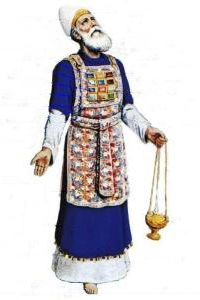
\includegraphics[width=50mm,scale=1.5]{Extras/Melchisedec.jpg}
\vspace{0.4in}  % Create a title for the document and write it in bold font
\LARGE{\textbf{\date}} % Again, do a line break
\linebreak 
% Create a subtitle \large{with Outlines, Statistics, Cross References, and Notes}
\vspace{0.5in}
\begin{flushleft}
\LARGE{Day \#100: Sunday, 10 April 2022 LITE \\}\vspace{0.25in}
\LARGE{2 Samuel 22-24 Psalm 100 Proverb 10}
\end{flushleft}
\vspace{0.6in}
\bigskip

\normalsize{Xenia, Oh.\\}
\normalsize{created: \today}
\vspace{1.3in}

\end{flushright}
\end{titlepage}

\newpage 
\tableofcontents\hypertarget{TOC}{}
\listoffigures
\listoftables

\hyphenation{A-bim-e-lech bre-thren E-phra-im  Gib-e-o-nites Jer-u-sa-lem through-out Phil-i-stines The-o-phil-us Am-a-le-kites ven-geance Mesh-el-e-mi-ah onan-ism Phar-a-oh thoughts grev-ous-ness Hach-a-liah adul-ter-er Shad-rach}

%%%%%%%%%%%%%%%%% EXTRA COLORS
%%%%%%%%%%%%%%%%% EXTRA COLORS
%%%%%%%%%%%%%%%%% EXTRA COLORS
\definecolor{champagne}{rgb}{0.97,0.91,0.81}
\definecolor{bone}{rgb}{0.89,0.85,0.79}

\definecolor{ForestGreen}{rgb}{0.00,0.29,0.098}
\definecolor{GIVING}{cmyk}{1,0.0,0.72,.1}

\definecolor{MLPE}{cmyk}{1,1,0,.45}
\definecolor{SOCCER}{cmyk}{.77, 0, .42, .49}
\definecolor{PAYBILL}{cmyk}{0,0.83,0.76,0.07}
\definecolor{SERMON}{cmyk}{.14,.9,0,.30} % aka seance \href{http://www.flatuicolorpicker.com/purple-cmyk-color-model/}{seance}
\definecolor{BIBLE}{cmyk}{0,.17,.74,.17}
\definecolor{WORKBLUE}{cmyk}{1, .5, 0, .6}
\definecolor{myOrange}{cmyk}{0, .4, .98, .03}
\definecolor{myTan}{cmyk}{0.0,.07,.17,.10}
\definecolor{myRed}{cmyk}{0,1,1,0}
\definecolor{myWhite}{cmyk}{0,0,0,0}
\definecolor{BLUESoD}{cmyk}{.97,.84,0,.04}
\definecolor{WHITE}{cmyk}{0,0,0,0}
\definecolor{OLDGOLD}{cmyk}{0.05,0.3,1.00,0}
\definecolor{CASTLETON}{cmyk}{1,0,0.31,0.66}
\definecolor{cadmiumgreen}{rgb}{0.0, 0.42, 0.24}
\definecolor{jungle}{rgb}{0.203,0.4882,0.1718}
\definecolor{MYGOLD}{rgb}{1,.84,0}

\definecolor{MYLIGHTGRAY}{rgb}{.85,.85,.85}

\definecolor{codegreen}{rgb}{0,0.6,0}
\definecolor{codegray}{rgb}{0.5,0.5,0.5}
\definecolor{codepurple}{rgb}{0.58,0,0.82}
\definecolor{backcolour}{rgb}{0.95,0.95,0.92}


\mdfdefinestyle{MyFrame}{%
    linecolor=blue,
    outerlinewidth=2pt,
    roundcorner=5pt,
    innertopmargin=\baselineskip,
    innerbottommargin=\baselineskip,
    innerrightmargin=10pt,
    innerleftmargin=10pt,
    backgroundcolor=gray!25!white}


\mdfdefinestyle{MyFrame2}{%
    linecolor=black,
    outerlinewidth=2pt,
    roundcorner=5pt,
    innertopmargin=\baselineskip,
    innerbottommargin=\baselineskip,
    innerrightmargin=10pt,
    innerleftmargin=10pt,
    backgroundcolor=yellow!25!white}


%%%%%
%% for PFTTIS list
%%%%%

%%% And Joseph said unto
\index[PFTTIS]{And Joseph said unto!Genesis!Gen 40:008}
\index[PFTTIS]{And Joseph said unto!Genesis!Gen 40:012}
\index[PFTTIS]{And Joseph said unto!Genesis!Gen 41:025}
\index[PFTTIS]{And Joseph said unto!Genesis!Gen 42:014}
\index[PFTTIS]{And Joseph said unto!Genesis!Gen 42:018}
\index[PFTTIS]{And Joseph said unto!Genesis!Gen 44:015}
\index[PFTTIS]{And Joseph said unto!Genesis!Gen 45:003}
\index[PFTTIS]{And Joseph said unto!Genesis!Gen 45:004}
\index[PFTTIS]{And Joseph said unto!Genesis!Gen 46:031}
\index[PFTTIS]{And Joseph said unto!Genesis!Gen 48:009}
\index[PFTTIS]{And Joseph said unto!Genesis!Gen 48:018}
\index[PFTTIS]{And Joseph said unto!Genesis!Gen 50:019}
\index[PFTTIS]{And Joseph said unto!Genesis!Gen 50:024}


%%% a shadow
\index[PFTTIS]{a shadow!1Chronicles!1Chr 029:15}
\index[PFTTIS]{a shadow!Job!Job 008:09}
\index[PFTTIS]{a shadow!Job!Job 014:02}
\index[PFTTIS]{a shadow!Job!Job 017:07}
\index[PFTTIS]{a shadow!Psalm!Psa 102:011}
\index[PFTTIS]{a shadow!Psalm!Psa 144:004}
\index[PFTTIS]{a shadow!Ecclesiastes!Eccl 006:012}
\index[PFTTIS]{a shadow!Ecclesiastes!Eccl 008:013}
\index[PFTTIS]{a shadow!Isaiah!Isa 04:006}
\index[PFTTIS]{a shadow!Isaiah!Isa 25:004}
\index[PFTTIS]{a shadow!Jonah!Jnh 04:06}
\index[PFTTIS]{a shadow!Colossians!Col 02:017}
\index[PFTTIS]{a shadow!Hebews!Heb 10:001}

%%% blessed is the man
\index[PFTTIS]{blessed is the man!Psalm!Psa 001:001}
\index[PFTTIS]{blessed is the man!Psalm!Psa 032:002}
\index[PFTTIS]{blessed is the man!Psalm!Psa 034:008}
\index[PFTTIS]{blessed is the man!Psalm!Psa 065:004}
\index[PFTTIS]{blessed is the man!Psalm!Psa 084:005}
\index[PFTTIS]{blessed is the man!Psalm!Psa 084:012}
\index[PFTTIS]{blessed is the man!Psalm!Psa 094:012}
\index[PFTTIS]{blessed is the man!Psalm!Psa 112:001}
\index[PFTTIS]{blessed is the man!Proverbs!Pro 008:034}
\index[PFTTIS]{blessed is the man!Isaiah!Isa 056:002}
\index[PFTTIS]{blessed is the man!Jeremiah!Jer 017:007}
\index[PFTTIS]{blessed is the man!Romans!Rom 004:008}
\index[PFTTIS]{blessed is the man!James!Jam 001:012}


%%% carry them
\index[PFTTIS]{carry them!Leviticus!Lev 14:045}
\index[PFTTIS]{carry them!Numbers!Num 11:012}
\index[PFTTIS]{carry them!Joshua!Jsh 04:003}
\index[PFTTIS]{carry them!1Samuel!1Sam 20:040}
\index[PFTTIS]{carry them!1Kings!1Kng 08:046}
\index[PFTTIS]{carry them!2Chronicles!2Chr 06:036}
\index[PFTTIS]{carry them!Ezra!Ezra 05:015}
\index[PFTTIS]{carry them!Isaiah!Isa 40:011}
\index[PFTTIS]{carry them!Isaiah!Isa 41:016}
\index[PFTTIS]{carry them!Isaiah!Isa 57:013}
\index[PFTTIS]{carry them!Jeremiah!Jer 20:004}
\index[PFTTIS]{carry them!Jeremiah!Jer 20:005}
\index[PFTTIS]{carry them!Jeremiah!Jer 43:012}


\index[PFTTIS]{good tidings!2Samuel!2Sam 18:027}
\index[PFTTIS]{good tidings!1Kings!1Ki 01:042}
\index[PFTTIS]{good tidings!2Kings!2Ki 07:009 (2x)}
\index[PFTTIS]{good tidings!Isaiah!Isa 40:009 (2x)}
\index[PFTTIS]{good tidings!Isaiah!Isa 41:007}
\index[PFTTIS]{good tidings!Isaiah!Isa 52:007}
\index[PFTTIS]{good tidings!Isaiah!Isa 61:001}
\index[PFTTIS]{good tidings!Nahum!Nah 01:005}
\index[PFTTIS]{good tidings!Luke!Lk 02:010}
\index[PFTTIS]{good tidings!1Thessalonians!1Thess 03:006}


%%% dead body
\index[PFTTIS]{dead body!Leviticus!Lev 21:011}
\index[PFTTIS]{dead body!Numbers!Num 06:006}
\index[PFTTIS]{dead body!Numbers!Num 09:006}
\index[PFTTIS]{dead body!Numbers!Num 09:007}
\index[PFTTIS]{dead body!Numbers!Num 09:010}
\index[PFTTIS]{dead body!Numbers!Num 09:011}
\index[PFTTIS]{dead body!Numbers!Num 09:013}
\index[PFTTIS]{dead body!Numbers!Num 09:016}
\index[PFTTIS]{dead body!2Kings!2Ki 08:005}
\index[PFTTIS]{dead body!Isaiah!Isa 26:019}
\index[PFTTIS]{dead body!Jeremiah!Jer 26:023}
\index[PFTTIS]{dead body!Jeremiah!Jer 36:030}
\index[PFTTIS]{dead body!Haggai!Hag 02:013}

%%% great sea
\index[PFTTIS]{great sea!Numbers!Num 34:006}
\index[PFTTIS]{great sea!Numbers!Num 34:007}
\index[PFTTIS]{great sea!Joshua!Jos 01:004}
\index[PFTTIS]{great sea!Joshua!Jos 09:001}
\index[PFTTIS]{great sea!Joshua!Jos 15:012}
\index[PFTTIS]{great sea!Joshua!Jos 15:047}
\index[PFTTIS]{great sea!Joshua!Jos 23:004}
\index[PFTTIS]{great sea!Ezekiel!Eze 47:010}
\index[PFTTIS]{great sea!Ezekiel!Eze 47:015}
\index[PFTTIS]{great sea!Ezekiel!Eze 47:019}
\index[PFTTIS]{great sea!Ezekiel!Eze 47:020}
\index[PFTTIS]{great sea!Ezekiel!Eze 48:028}
\index[PFTTIS]{great sea!Daniel!Dan 07:002}


%%% have forsaken me
\index[PFTTIS]{have forsaken me!Judges!Jdg 10:013}
\index[PFTTIS]{have forsaken me!1Samuel!1Sam 08:008}
\index[PFTTIS]{have forsaken me!1Kings!1Ki 11:033}
\index[PFTTIS]{have forsaken me!2Kings!2Ki 22:017}
\index[PFTTIS]{have forsaken me!2Chronicles!2Chr 12:005}
\index[PFTTIS]{have forsaken me!2Chronicles!2Chr 34:025}
\index[PFTTIS]{have forsaken me!Jeremiah!Jer 01:016}
\index[PFTTIS]{have forsaken me!Jeremiah!Jer 02:013}
\index[PFTTIS]{have forsaken me!Jeremiah!Jer 05:007}
\index[PFTTIS]{have forsaken me!Jeremiah!Jer 05:019}
\index[PFTTIS]{have forsaken me!Jeremiah!Jer 16:011 (2x)}
\index[PFTTIS]{have forsaken me!Jeremiah!Jer 19:004}

%%% no king
\index[PFTTIS]{no king!Judges!Jdg 17:06}
\index[PFTTIS]{no king!Judges!Jdg 18:01}
\index[PFTTIS]{no king!Judges!Jdg 19:01}
\index[PFTTIS]{no king!Judges!Jdg 21:25}
\index[PFTTIS]{no king!1Kings!1Ki 22:47}
\index[PFTTIS]{no king!2Kings!2Ki 23:25}
\index[PFTTIS]{no king!Nehemiah!Neh 13:26}
\index[PFTTIS]{no king!Psalms!Psa 033:016}
\index[PFTTIS]{no king!Proverbs!Pro 30:27}
\index[PFTTIS]{no king!Daniel!Dan 02:10}
\index[PFTTIS]{no king!Hosea!Hos 10:03}
\index[PFTTIS]{no king!Micah!Mic 04:09}
\index[PFTTIS]{no king!John!Jhn 19:15}


%%% rebellious house
\index[PFTTIS]{rebellious house!Exodus!Exo 02:005}
\index[PFTTIS]{rebellious house!Exodus!Exo 02:006}
\index[PFTTIS]{rebellious house!Exodus!Exo 02:008}
\index[PFTTIS]{rebellious house!Exodus!Exo 03:009}
\index[PFTTIS]{rebellious house!Exodus!Exo 03:026}
\index[PFTTIS]{rebellious house!Exodus!Exo 03:027}
\index[PFTTIS]{rebellious house!Exodus!Exo 12:002 (2x)}
\index[PFTTIS]{rebellious house!Exodus!Exo 12:003}
\index[PFTTIS]{rebellious house!Exodus!Exo 12:009}
\index[PFTTIS]{rebellious house!Exodus!Exo 12:025}
\index[PFTTIS]{rebellious house!Exodus!Exo 17:012}
\index[PFTTIS]{rebellious house!Exodus!Exo 24:003}

%%% seek him
\index[PFTTIS]{seek him!Deuteronomy!Deu 04:029}\index[PFTTIS]{seek him!1Samuel!1Sam 23:025}
\index[PFTTIS]{seek him!1Chronicles!1Chr 28:009}
\index[PFTTIS]{seek him!2Chronicles!1Chr 15:002}
\index[PFTTIS]{seek him!Ezra!Ezr 08:022}
\index[PFTTIS]{seek him!Psalms!Psa 022:026}
\index[PFTTIS]{seek him!Psalms!Psa 024:006}
\index[PFTTIS]{seek him!Psalms!Psa 119:002}
\index[PFTTIS]{seek him!SoS!SoS 03:002}
\index[PFTTIS]{seek him!SoS!SoS 06:001}
\index[PFTTIS]{seek him!Hosea!Hos 07:010}
\index[PFTTIS]{seek him!Amos!Amo 05:008}
\index[PFTTIS]{seek him!Hebrews!Heb 11:0063}


%%% seek ye
\index[PFTTIS]{seek ye!Isaiah!Isa 34:016}
\index[PFTTIS]{seek ye!Isaiah!Isa 45:019}
\index[PFTTIS]{seek ye!Isaiah!Isa 55:006}
\index[PFTTIS]{seek ye!Amos!Amos 5:004}
\index[PFTTIS]{seek ye!John!John 1:38}
\index[PFTTIS]{seek ye!John!John 18:4}
\index[PFTTIS]{seek ye!John!John 18:7}
\index[PFTTIS]{seek ye!Matthew!Matt 6:33}
\index[PFTTIS]{seek ye!Numbers!Num 16:10}
\index[PFTTIS]{seek ye!Luke!Luke 12:31}
\index[PFTTIS]{seek ye!Luke!Luke 24:5}
\index[PFTTIS]{seek ye!Psalm!Psa 27:8}
\index[PFTTIS]{seek ye!Zephaniah!Zeph 2:3}

%%% the uncircumcised
\index[PFTTIS]{the uncircumcised!Genesis!Gen 17:014}
\index[PFTTIS]{the uncircumcised!Judges!Jdg 14:003}
\index[PFTTIS]{the uncircumcised!Judges!Jdg 15:018}
\index[PFTTIS]{the uncircumcised!2Samuel!2Sam 01:020}
\index[PFTTIS]{the uncircumcised!Isaiah!Isa 02:001}
\index[PFTTIS]{the uncircumcised!Jeremiah!Jer 09:025}
\index[PFTTIS]{the uncircumcised!Ezekiel!Eze 28:010}
\index[PFTTIS]{the uncircumcised!Ezekiel!Eze 31:018}
\index[PFTTIS]{the uncircumcised!Ezekiel!Eze 32:019}
\index[PFTTIS]{the uncircumcised!Ezekiel!Eze 32:027}
\index[PFTTIS]{the uncircumcised!Ezekiel!Eze 32:028}
\index[PFTTIS]{the uncircumcised!Ezekiel!Eze 32:029}
\index[PFTTIS]{the uncircumcised!Ezekiel!Eze 32:032}

%%% worship him
\index[PFTTIS]{worship him!Psalms!Psa 97:007}
\index[PFTTIS]{worship him!Zephaniah!Zeph 02:011}
\index[PFTTIS]{worship him!Matthew!Matt 02:002}
\index[PFTTIS]{worship him!Matthew!Matt 02:008}
\index[PFTTIS]{worship him!John!John 04:023}
\index[PFTTIS]{worship him!John!John 04:024 (2x)} 
\index[PFTTIS]{worship him!Acts!Acts 17:023}
\index[PFTTIS]{worship him!Hebrews!Heb 01:006}
\index[PFTTIS]{worship him!Revelation!Rev 04:010}
\index[PFTTIS]{worship him!Revelation!Rev 13:008}
\index[PFTTIS]{worship him!Revelation!Rev 14:007}
\index[PFTTIS]{worship him!Revelation!Rev 19:010}


%%%%%
%% for PFTTIS list
%%%%%

%%% afflictions
\index[WFTTIS]{afflictions!Psalms!Psa 34:019}
\index[WFTTIS]{afflictions!Psalms!Psa 132:001}
\index[WFTTIS]{afflictions!Acts!Acts 07:010}
\index[WFTTIS]{afflictions!Acts!Acts 20:023}
\index[WFTTIS]{afflictions!2Corinthians!2Cor 06:004}
\index[WFTTIS]{afflictions!Colossians!Col 01:024}
\index[WFTTIS]{afflictions!1Thessalonians!1Thess 03:003}
\index[WFTTIS]{afflictions!2Timothy!2Tim 01:008}
\index[WFTTIS]{afflictions!2Timothy!2Tim 03:011}
\index[WFTTIS]{afflictions!2Timothy!2Tim 04:005}
\index[WFTTIS]{afflictions!Hebrews!Heb 10:032}
\index[WFTTIS]{afflictions!Hebrews!Heb 10:033}
\index[WFTTIS]{afflictions!1Peter!1Pet 05:009}

%%% acsend
\index[WFTTIS]{acsend!Joshua!Jos 06:05}
\index[WFTTIS]{acsend!Psalm!Psa 024:003}
\index[WFTTIS]{acsend!Psalm!Psa 135:007}
\index[WFTTIS]{acsend!Psalm!Psa 139:008}
\index[WFTTIS]{acsend!Isaiah!Isa 14:013}
\index[WFTTIS]{acsend!Isaiah!Isa 14:014}
\index[WFTTIS]{acsend!Jeremiah!Jer 10:013}
\index[WFTTIS]{acsend!Jeremiah!Jer 51:016}
\index[WFTTIS]{acsend!Ezekiel!Eze 38:009}
\index[WFTTIS]{acsend!John!John 06:062}
\index[WFTTIS]{acsend!John!John 20:017}
\index[WFTTIS]{acsend!Romans!Rom 10:006}
\index[WFTTIS]{acsend!Revelation!Rev 17:008}

%%% Assyrian
\index[WFTTIS]{Assyrian!Isaiah!Isa 10:005}
\index[WFTTIS]{Assyrian!Isaiah!Isa 10:024}
\index[WFTTIS]{Assyrian!Isaiah!Isa 14:025}
\index[WFTTIS]{Assyrian!Isaiah!Isa 19:023}
\index[WFTTIS]{Assyrian!Isaiah!Isa 23:013}
\index[WFTTIS]{Assyrian!Isaiah!Isa 30:031}
\index[WFTTIS]{Assyrian!Isaiah!Isa 31:008}
\index[WFTTIS]{Assyrian!Isaiah!Isa 52:004}
\index[WFTTIS]{Assyrian!Ezekiel!Eze 31:003}
\index[WFTTIS]{Assyrian!Hosea!Hos 05:013}
\index[WFTTIS]{Assyrian!Hosea!Hos 11:005}
\index[WFTTIS]{Assyrian!Micah!Hos 05:005}
\index[WFTTIS]{Assyrian!Micah!Hos 05:006}

%%% blot
\index[WFTTIS]{blot!Exodus!Exo 32:032}
\index[WFTTIS]{blot!Exodus!Exo 32:033}
\index[WFTTIS]{blot!Numbers!Num 05:026}
\index[WFTTIS]{blot!Deuteronomy!Deut 09:014}
\index[WFTTIS]{blot!Deuteronomy!Deut 25:019}
\index[WFTTIS]{blot!Deuteronomy!Deut 29:020}
\index[WFTTIS]{blot!2Kings!2Ki 14:027}
\index[WFTTIS]{blot!Job!Job 31:007}
\index[WFTTIS]{blot!Psalms!Psa 51:001}
\index[WFTTIS]{blot!Psalms!Psa 51:009}
\index[WFTTIS]{blot!Proverbs!Pro 09:007}
\index[WFTTIS]{blot!Jeremiah!Jer 18:023}
\index[WFTTIS]{blot!Revelation!Rev 03:005}


%%% chain
\index[WFTTIS]{chain!Genesis!Gen 41:042}
\index[WFTTIS]{chain!1Kings!1Ki 07:017}
\index[WFTTIS]{chain!Psalms!Psa 73:006}
\index[WFTTIS]{chain!SoS!Sos 04:009}
\index[WFTTIS]{chain!Lamentations!Lam 03:007}
\index[WFTTIS]{chain!Ezekiel!Eze 07:023}
\index[WFTTIS]{chain!Ezekiel!Eze 16:011}
\index[WFTTIS]{chain!Daniel!Dan 05:007}
\index[WFTTIS]{chain!Daniel!Dan 05:016}
\index[WFTTIS]{chain!Daniel!Dan 05:029}
\index[WFTTIS]{chain!Acts!Acts 28:020}
\index[WFTTIS]{chain!2Timothy!2Tim 01:016}
\index[WFTTIS]{chain!Revelation!Rev 20:001}


%%% controversy
\index[WFTTIS]{controversy!Deuteronomy!Deu 17:008}
\index[WFTTIS]{controversy!Deuteronomy!Deu 19:017}
\index[WFTTIS]{controversy!Deuteronomy!Deu 21:005}
\index[WFTTIS]{controversy!Deuteronomy!Deu 25:001}
\index[WFTTIS]{controversy!2Samuel!2Sam 15:002}
\index[WFTTIS]{controversy!Isaiah!Isa 34:008}
\index[WFTTIS]{controversy!Jeremiah!Jer 25:031}
\index[WFTTIS]{controversy!Ezekiel!Eze 44:024}
\index[WFTTIS]{controversy!Hosea!Hos 04:001}
\index[WFTTIS]{controversy!Hosea!Hos 12:002}
\index[WFTTIS]{controversy!Micah!Mic 06:002 (2x)}
\index[WFTTIS]{controversy!1Timothy!1Tim 03:016}


%%% Dagon/Dagon's
\index[WFTTIS]{Dagon!Judges!Jdg 16:023}
\index[WFTTIS]{Dagon!1Samuel!1Sam 05:002 (2x)}
\index[WFTTIS]{Dagon!1Samuel!1Sam 05:003 (2x)}
\index[WFTTIS]{Dagon!1Samuel!1Sam 05:004 (3x)}
\index[WFTTIS]{Dagon!1Samuel!1Sam 05:005 (3x)}
\index[WFTTIS]{Dagon!1Samuel!1Sam 05:007}
\index[WFTTIS]{Dagon!1Chronicles!1Chr 10:010}

%%% disobedient
\index[WFTTIS]{disobedient!1Kings!1Ki 13:026}
\index[WFTTIS]{disobedient!Nehemiah!Neh 09:026}
\index[WFTTIS]{disobedient!Luke!Luke 01:017}
\index[WFTTIS]{disobedient!Acts!Acts 26:019}
\index[WFTTIS]{disobedient!Romans!Rom 01:030}
\index[WFTTIS]{disobedient!Romans!Rom 10:021}
\index[WFTTIS]{disobedient!1Timothy!1Tim 01:009}
\index[WFTTIS]{disobedient!2Timothy!2Tim 03:002}
\index[WFTTIS]{disobedient!Titus!Titus 01:016}
\index[WFTTIS]{disobedient!Titus!Titus 03:003}
\index[WFTTIS]{disobedient!1Peter!1Pet 02:007}
\index[WFTTIS]{disobedient!1Peter!1Pet 02:008}
\index[WFTTIS]{disobedient!1Peter!1Pet 03:020}


%%% doubt
\index[WFTTIS]{doubt!Genesis!Gen 37:033}
\index[WFTTIS]{doubt!Deuteronomy!Deu 28:066}
\index[WFTTIS]{doubt!Job!Job 12:002}
\index[WFTTIS]{doubt!Matthew!Matt 14:031}
\index[WFTTIS]{doubt!Matthew!Matt 21:021}
\index[WFTTIS]{doubt!Mark!Mk 11:023}
\index[WFTTIS]{doubt!Luke!Lk 11:020}
\index[WFTTIS]{doubt!John!Jhn 10:024}
\index[WFTTIS]{doubt!Acts!Acts 02:012}
\index[WFTTIS]{doubt!Acts!Acts 28:004}
\index[WFTTIS]{doubt!1Corinthians!1Cor 09:010}
\index[WFTTIS]{doubt!Galatians!Gal 04:020}
\index[WFTTIS]{doubt!1John!1Jhn 02:019}


%%% dungeon
\index[WFTTIS]{dungeon!Genesis!Gen 40:015}
\index[WFTTIS]{dungeon!Genesis!Gen 41:014}
\index[WFTTIS]{dungeon!Exodus!Exo 12:029}
\index[WFTTIS]{dungeon!Jeremiah!Jer 37:016}
\index[WFTTIS]{dungeon!Jeremiah!Jer 38:006 (2x)}
\index[WFTTIS]{dungeon!Jeremiah!Jer 38:007}
\index[WFTTIS]{dungeon!Jeremiah!Jer 38:009}
\index[WFTTIS]{dungeon!Jeremiah!Jer 38:010}
\index[WFTTIS]{dungeon!Jeremiah!Jer 38:011}
\index[WFTTIS]{dungeon!Jeremiah!Jer 38:013}
\index[WFTTIS]{dungeon!Lamentations!Lam 03:053}
\index[WFTTIS]{dungeon!Lamentations!Lam 03:055}


%%% error
\index[WFTTIS]{error!2Samuel!2Sam 06:007}
\index[WFTTIS]{error!Job!Job 19:004}
\index[WFTTIS]{error!Ecclesiastes!Ecc 05:006}
\index[WFTTIS]{error!Ecclesiastes!Ecc 10:005}
\index[WFTTIS]{error!Isaiah!Isa 32:006}
\index[WFTTIS]{error!Daniel!Dan 06:004}
\index[WFTTIS]{error!Matthew!Matt 27:064}
\index[WFTTIS]{error!Romans!Rom 01:027}
\index[WFTTIS]{error!James!Jam 05:020}
\index[WFTTIS]{error!2Peter!2Pet 02:018}
\index[WFTTIS]{error!2Peter!2Pet 03:017}
\index[WFTTIS]{error!1John!1Jn 04:006}
\index[WFTTIS]{error!Jude!Jude 01:011}

%%% fourish
\index[WFTTIS]{fourish!Psalms!Psa 072:007}
\index[WFTTIS]{fourish!Psalms!Psa 072:016}
\index[WFTTIS]{fourish!Psalms!Psa 092:007}
\index[WFTTIS]{fourish!Psalms!Psa 092:012}
\index[WFTTIS]{fourish!Psalms!Psa 092:013}
\index[WFTTIS]{fourish!Psalms!Psa 132:018}
\index[WFTTIS]{fourish!Proverbs!Pro 11:28}
\index[WFTTIS]{fourish!Proverbs!Pro 14:11}
\index[WFTTIS]{fourish!Ecclesiastes!Ecc 12:05}
\index[WFTTIS]{fourish!SongOfSolomon!SOS 07:12}
\index[WFTTIS]{fourish!Isaiah!Isa 17:11}
\index[WFTTIS]{fourish!Isaiah!Isa 66:14}
\index[WFTTIS]{fourish!Ezekiel!Eze 17:24}




%%% giants
\index[WFTTIS]{giants!Genesis!Gen 06:004}
\index[WFTTIS]{giants!Numbers!Num 13:033}
\index[WFTTIS]{giants!Deuteronomy!Deut 02:011}
\index[WFTTIS]{giants!Deuteronomy!Deut 02:021}
\index[WFTTIS]{giants!Deuteronomy!Deut 03:011}
\index[WFTTIS]{giants!Deuteronomy!Deut 03:013}
\index[WFTTIS]{giants!Joshua!Josh 12:004}
\index[WFTTIS]{giants!Joshua!Josh 13:012}
\index[WFTTIS]{giants!Joshua!Josh 15:008}
\index[WFTTIS]{giants!Joshua!Josh 17:015}
\index[WFTTIS]{giants!Joshua!Josh 16:016}

%%% good man
\index[WFTTIS]{good man!2 Samuel!2Sa 18:27}
%(1) Psalms 37:23 [5]
%(1) Psalms 112:5 [2]
%(1) Proverbs 12:2 [2]
%(1) Proverbs 13:22 [2]
%(1) Proverbs 14:14 [14]
%(1) Micah 7:2 [2]
%(1) Matthew 12:35 [2]
%(1) Luke 6:45 [2]
%(1) Luke 23:50 [15]
%(1) John 7:12 [17]
%(1) Acts 11:24 [5]
%(1) Romans 5:7 [14]

%%% Hinnom
\index[WFTTIS]{Hinnom!Joshua!Jsh 15:008}
\index[WFTTIS]{Hinnom!Joshua!Jsh 18:016}
\index[WFTTIS]{Hinnom!2Kings!2Ki 23:010}
\index[WFTTIS]{Hinnom!2Chronicles!2Chr 28:003}
\index[WFTTIS]{Hinnom!2Chronicles!2Chr 33:006}
\index[WFTTIS]{Hinnom!Nehemiah!Neh 11:030}
\index[WFTTIS]{Hinnom!Jeremiah!Jer 07:031}
\index[WFTTIS]{Hinnom!Jeremiah!Jer 07:032}
\index[WFTTIS]{Hinnom!Jeremiah!Jer 19:002}
\index[WFTTIS]{Hinnom!Jeremiah!Jer 19:006}
\index[WFTTIS]{Hinnom!Jeremiah!Jer 32:035}

%%% inclined
\index[WFTTIS]{inclined!Judges!Jdg 09:003}
\index[WFTTIS]{inclined!Psalms!Psa 040:001}
\index[WFTTIS]{inclined!Psalms!Psa 116:002}
\index[WFTTIS]{inclined!Psalms!Psa 119:112}
\index[WFTTIS]{inclined!Proverbs!Pro 05:13}
\index[WFTTIS]{inclined!Jeremiah!Jer 07:24}
\index[WFTTIS]{inclined!Jeremiah!Jer 07:26}
\index[WFTTIS]{inclined!Jeremiah!Jer 11:08}
\index[WFTTIS]{inclined!Jeremiah!Jer 17:23}
\index[WFTTIS]{inclined!Jeremiah!Jer 25:04}
\index[WFTTIS]{inclined!Jeremiah!Jer 34:14}
\index[WFTTIS]{inclined!Jeremiah!Jer 35:15}
\index[WFTTIS]{inclined!Jeremiah!Jer 44:05}


%%% laughed
\index[WFTTIS]{laughed!Genesis!Gen 17:017}
\index[WFTTIS]{laughed!Genesis!Gen 18:012}
\index[WFTTIS]{laughed!Genesis!Gen 18:015}
\index[WFTTIS]{laughed!2Kings!2Ki 19:021}
\index[WFTTIS]{laughed!2Chronicles!2Chr 30:010}
\index[WFTTIS]{laughed!Nehemiah!Neh 02:019}
\index[WFTTIS]{laughed!Job!Job 12:004}
\index[WFTTIS]{laughed!Job!Job 29:024}
\index[WFTTIS]{laughed!Isaiah!Isa 37:022}
\index[WFTTIS]{laughed!Ezekiel!Ezek 23:032}
\index[WFTTIS]{laughed!Matthew!Matt 09:024}
\index[WFTTIS]{laughed!Mark!Mk 05:040}
\index[WFTTIS]{laughed!Luke!Lk 08:053}

%%% liar
\index[WFTTIS]{liar!Job!Job 24:025}
\index[WFTTIS]{liar!Proverbs!Pro 17:004}
\index[WFTTIS]{liar!Proverbs!Pro 19:022}
\index[WFTTIS]{liar!Proverbs!Pro 30:006}
\index[WFTTIS]{liar!Jeremiah!Jer 15:018}
\index[WFTTIS]{liar!John!Jhn 08:044}
\index[WFTTIS]{liar!John!Jhn 08:055}
\index[WFTTIS]{liar!Romans!Rom 03:004}
\index[WFTTIS]{liar!1John!1Jhn 01:010}
\index[WFTTIS]{liar!1John!1Jhn 02:004}
\index[WFTTIS]{liar!1John!1Jhn 02:022}
\index[WFTTIS]{liar!1John!1Jhn 04:020}
\index[WFTTIS]{liar!1John!1Jhn 05:010}

%%% palsy
\index[WFTTIS]{palsy!Matthew!Matt 04:024}
\index[WFTTIS]{palsy!Matthew!Matt 08:006}
\index[WFTTIS]{palsy!Matthew!Matt 09:002}
\index[WFTTIS]{palsy!Matthew!Matt 09:006}
\index[WFTTIS]{palsy!Mark!Mk 02:003}
\index[WFTTIS]{palsy!Mark!Mk 02:004}
\index[WFTTIS]{palsy!Mark!Mk 02:005}
\index[WFTTIS]{palsy!Mark!Mk 02:009}
\index[WFTTIS]{palsy!Mark!Mk 02:010}
\index[WFTTIS]{palsy!Luke!Lk 05:018}
\index[WFTTIS]{palsy!Luke!Lk 05:024}
\index[WFTTIS]{palsy!Acts!Acts 09:033}

%%% Profitable
\index[WFTTIS]{profitable!Job!Job 22:002 (2x)}
\index[WFTTIS]{profitable!Ecclesiastes!Ecc 10:010}
\index[WFTTIS]{profitable!Isaiah!Isa 44:010}
\index[WFTTIS]{profitable!Jeremiah!Jer 13:007}
\index[WFTTIS]{profitable!Matthew!Matt 05:029}
\index[WFTTIS]{profitable!Matthew!Matt 05:030}
\index[WFTTIS]{profitable!Acts!Acts 20:020}
\index[WFTTIS]{profitable!1Timothy!1Tim 04:008}
\index[WFTTIS]{profitable!2Timothy!2Tim 03:016}
\index[WFTTIS]{profitable!2Timothy!2Tim 04:011}
\index[WFTTIS]{profitable!Titus!Titus 03:008}
\index[WFTTIS]{profitable!Philemon!Phlm 01:011}

%%% Rechab
\index[WFTTIS]{Rechab!2Samuel!2Sam 04:002}
\index[WFTTIS]{Rechab!2Samuel!2Sam 04:005}
\index[WFTTIS]{Rechab!2Samuel!2Sam 04:006}
\index[WFTTIS]{Rechab!2Samuel!2Sam 04:009}
\index[WFTTIS]{Rechab!2KIngs!2Ki 10:015}
\index[WFTTIS]{Rechab!2KIngs!2Ki 10:023}
\index[WFTTIS]{Rechab!1Chronicles!1Chr 02:055}
\index[WFTTIS]{Rechab!Nehemiah!Neh 03:014}
\index[WFTTIS]{Rechab!Jeremiah!Jer 35:006}
\index[WFTTIS]{Rechab!Jeremiah!Jer 35:008}
\index[WFTTIS]{Rechab!Jeremiah!Jer 35:014}
\index[WFTTIS]{Rechab!Jeremiah!Jer 35:016}
\index[WFTTIS]{Rechab!Jeremiah!Jer 35:019}

%%% serpents
\index[WFTTIS]{serpents!Exodus!Exo 07:012}
\index[WFTTIS]{serpents!Numbers!Num 21:006}
\index[WFTTIS]{serpents!Numbers!Num 21:007}
\index[WFTTIS]{serpents!Deuteronomy!Deu 08:015}
\index[WFTTIS]{serpents!Deuteronomy!Deu 32:024}
\index[WFTTIS]{serpents!Jeremiah!Jer 08:017}
\index[WFTTIS]{serpents!Matthew!Matt 10:016}
\index[WFTTIS]{serpents!Matthew!Matt 23:033}
\index[WFTTIS]{serpents!Mark!Mk 16:018}
\index[WFTTIS]{serpents!Luke!Lk 10:019}
\index[WFTTIS]{serpents!1Corinthians!1Cor 10:009}
\index[WFTTIS]{serpents!James!Jas 03:007}
\index[WFTTIS]{serpents!Revelation!Rev 09:019}

%%% short
\index[WFTTIS]{short!Numbers!Num 11:023}
\index[WFTTIS]{short!2Kings!2Ki 10:032}
\index[WFTTIS]{short!Job!Job 17:012}
\index[WFTTIS]{short!Job!Job 20:005}
\index[WFTTIS]{short!Psalms!Psa 89:047}
\index[WFTTIS]{short!Romans!Rom 03:023}
\index[WFTTIS]{short!Romans!Rom 09:028  (2x)}
\index[WFTTIS]{short!1Corinthians!1Cor 07:029}
\index[WFTTIS]{short!1Thessalonians!1Thess 02:017}
\index[WFTTIS]{short!Hebrews!Heb 04:001}
\index[WFTTIS]{short!Revelation!Rev 12:012}
\index[WFTTIS]{short!Revelation!Rev 17:010}

%%% smiteth
\index[WFTTIS]{smiteth!Exodus!Exo 21:012}
\index[WFTTIS]{smiteth!Exodus!Exo 21:15}
\index[WFTTIS]{smiteth!Deuteronomy!Dt 25:11}
\index[WFTTIS]{smiteth!Deuteronomy!Dt 27:24}
\index[WFTTIS]{smiteth!Joshua!Jsh 15:16}
\index[WFTTIS]{smiteth!Judges!Jdg 15:16}
\index[WFTTIS]{smiteth!2 Samuel!2Sa 05:08}
\index[WFTTIS]{smiteth!1Chronicles!1Chr 11:06}
\index[WFTTIS]{smiteth!Job!1Chr 26:12}
\index[WFTTIS]{smiteth!Isaiah!Isa 09:13}
\index[WFTTIS]{smiteth!Lamentations!Lam 03:30}
\index[WFTTIS]{smiteth!Ezekiel!Eze 07:09}
\index[WFTTIS]{smiteth!Luke!Lk 06:29}



%%% vanities
\index[WFTTIS]{vanities!Deuteronomy!Deut 21:021}
\index[WFTTIS]{vanities!1Kings!1Ki 16:013}
\index[WFTTIS]{vanities!1Kings!1Ki 16:026}
\index[WFTTIS]{vanities!Psalms!Psa 031:006}
\index[WFTTIS]{vanities!Ecclesiastes!Ecc 01:002 (2x)}
\index[WFTTIS]{vanities!Ecclesiastes!Ecc 05:007}
\index[WFTTIS]{vanities!Ecclesiastes!Ecc 12:008}
\index[WFTTIS]{vanities!Jeremiah!Jer 08:019}
\index[WFTTIS]{vanities!Jeremiah!Jer 10:008}
\index[WFTTIS]{vanities!Jeremiah!Jer 14:022}
\index[WFTTIS]{vanities!Jonah!Jnh 02:008}
\index[WFTTIS]{vanities!Acts!Acts 14:015}



%%%%%
%% for PFTTIS list
%%%%%

%%% worm
\index[WFITV]{worm!Exodus!Exo 16:024}
\index[WFITV]{worm!Job!Job 17:014}
\index[WFITV]{worm!Job!Job 24:029}
\index[WFITV]{worm!Job!Job 25:005 (2x)}
\index[WFITV]{worm!Psalms!Psa 022:006}
\index[WFITV]{worm!Isaiah!Isa 14:011}
\index[WFITV]{worm!Isaiah!Isa 41:014}
\index[WFITV]{worm!Isaiah!Isa 51:008}
\index[WFITV]{worm!Isaiah!Isa 66:024}
\index[WFITV]{worm!Jonah!Jnh 04:007}
\index[WFITV]{worm!Mark!Mk 09:044}
\index[WFITV]{worm!Mark!Mk 09:046}
\index[WFITV]{worm!Mark!Mk 09:048}


%\subsubsection{Title}
%\textbf{Introduction:} Isaiah 46 
%\index[speaker]{Speaker!Isaiah 49 (Title}
%\index[series]{Book (Speaker)!IPassage (Title)}
%\index[date]{2017/07/09!Isaiah 49 (Title)}
%\begin{compactenum}[I.]
%    \item  \textbf{Point} \index[scripture]{Isaiah!IPassage} (IPassage)
%\end{compactenum}




  

\chapter{2 Samuel 22}

\begin{figure}
  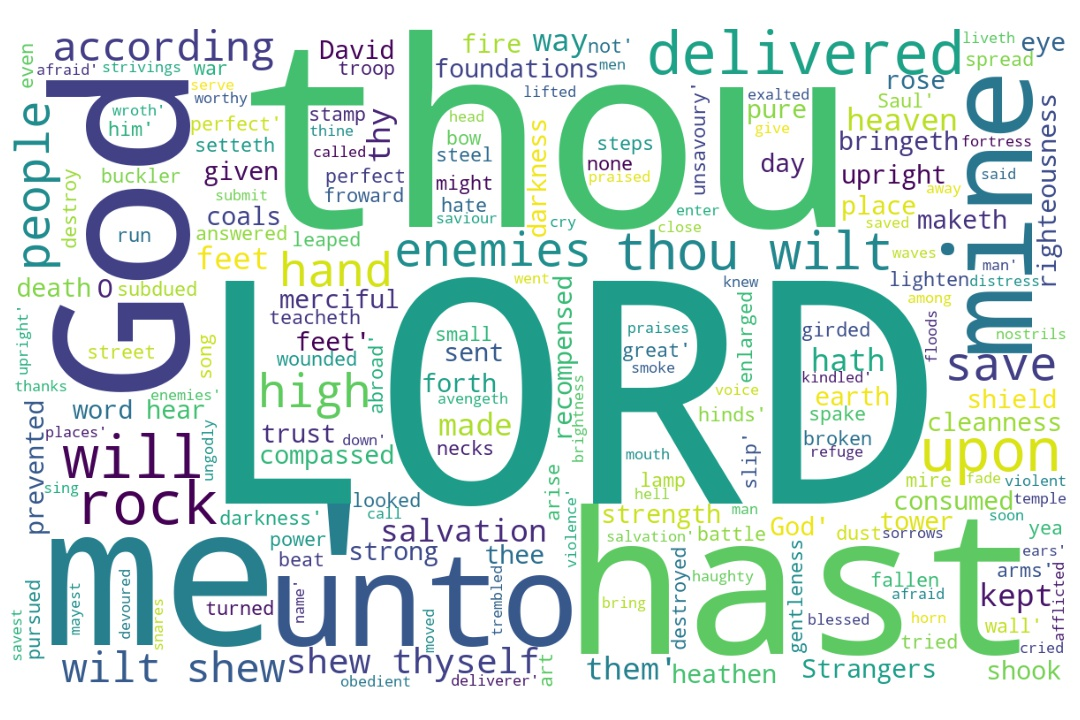
\includegraphics[width=\linewidth]{10OT-2Samuel/2Samuel22-WordCloud.jpg}
  \caption{1 Samuel 22 Word Cloud}
  \label{fig:1 Samuel 22 Word Cloud}
\end{figure}

%%%%%%%%%%%%%%%%%%%%%%%%%%%%%%%%%%%%%%%%%
%%%%%%%%%%%%%%%%%%%%%%%%%%%%%%%%%%%%%%%%%

\marginpar{\scriptsize \centering \fcolorbox{bone}{lime}{\textbf{DAVID"S REFLECTION}}\\ (2 Samuel 22:1--51) 
\begin{compactenum}[I.][8]
    \item David as a  \textbf{Vessel} %\index[scripture]{2Samuel!2Sa 22:01}(2Sa 22:1) 
    \item Two \textbf{Voices}  \index[scripture]{2Samuel!2Sa 22:07}  \index[scripture]{2Samuel!2Sa 22:14} (2Sa 22:7, 14) 
    \item The \textbf{Virtue} (or lack thereof, and the rewards thereof, but the repentance \index[scripture]{2Samuel!2Sa 22:22--26}(2Sa  22:22--26) 
    \item God's Care for \textbf{Victims}  \index[scripture]{2Samuel!2Sa 22:28}(2Sa 22:28) 
    \item The \textbf{Victories}  \index[scripture]{2Samuel!2Sa 22:40}(2Sa 22:40) 
    \item An \textbf{Avenging}  \index[scripture]{2Samuel!2Sa 22:48}(2Sa 22:48) 
    \item Deliverance from the  \textbf{Violent}  \index[scripture]{2Samuel!2Sa 22:49}(2Sa 22:49) 
\end{compactenum} }

\footnote{\textcolor[cmyk]{0.99998,1,0,0}{\hyperlink{TOC}{Return to end of Table of Contents.}}}\footnote{\href{https://audiobible.com/bible/2_samuel_22.html}{\textcolor[cmyk]{0.99998,1,0,0}{2 Samuel 22 Audio}}}\textcolor[cmyk]{0.99998,1,0,0}{And David spake unto the LORD the words of this song in the day \emph{that} the LORD had delivered him out of the hand of all his enemies, and out of the hand of Saul:}
[2] \textcolor[cmyk]{0.99998,1,0,0}{And he said, The LORD \emph{is} my rock, and my fortress, and my deliverer;}
[3] \textcolor[cmyk]{0.99998,1,0,0}{The God of my rock; in him will I trust: \emph{he} \emph{is} my shield, and the horn of my salvation, my high tower, and my refuge, my saviour; \fcolorbox{bone}{bone}{thou}  savest me from violence.}
[4] \textcolor[cmyk]{0.99998,1,0,0}{I will call on the LORD, \emph{who} \emph{is} worthy to be praised: so shall I be saved from mine enemies.}
[5] \textcolor[cmyk]{0.99998,1,0,0}{When the waves of death compassed me, the floods of ungodly men made me afraid;}
[6] \textcolor[cmyk]{0.99998,1,0,0}{The sorrows of hell compassed me about; the snares of death prevented me;}
[7] \textcolor[cmyk]{0.99998,1,0,0}{In my distress I called upon the LORD, and cried to my God: and he did hear \fcolorbox{bone}{lime}{my voice} out of his temple, and my cry \emph{did} \emph{enter} into his ears.}
[8] \textcolor[cmyk]{0.99998,1,0,0}{Then the earth shook and trembled; the foundations of heaven moved and shook, because he was wroth.}
[9] \textcolor[cmyk]{0.99998,1,0,0}{There went up a smoke out of his nostrils, and fire out of his mouth devoured: coals were kindled by it.}
[10] \textcolor[cmyk]{0.99998,1,0,0}{He bowed the heavens also, and came down; and darkness \emph{was} under his feet.}
[11] \textcolor[cmyk]{0.99998,1,0,0}{And he rode upon a cherub, and did fly: and he was seen upon the wings of the wind.}
[12] \textcolor[cmyk]{0.99998,1,0,0}{And he made darkness pavilions round about him, dark waters, \emph{and} thick clouds of the skies.}
[13] \textcolor[cmyk]{0.99998,1,0,0}{Through the brightness before him were coals of fire kindled.}
[14] \textcolor[cmyk]{0.99998,1,0,0}{The LORD thundered from heaven, and the most High uttered \fcolorbox{bone}{lime}{his voice}.}
[15] \textcolor[cmyk]{0.99998,1,0,0}{And he sent out arrows, and scattered them; lightning, and discomfited them.}
[16] \textcolor[cmyk]{0.99998,1,0,0}{And the channels of the sea appeared, the foundations of the world were discovered, at the rebuking of the LORD, at the blast of the breath of his nostrils.}
[17] \textcolor[cmyk]{0.99998,1,0,0}{He sent from above, he took me; he drew me out of many waters;}
[18] \textcolor[cmyk]{0.99998,1,0,0}{He delivered me from my strong enemy, \emph{and} from them that hated me: for they were too strong for me.}
[19] \textcolor[cmyk]{0.99998,1,0,0}{They prevented me in the day of my calamity: but the LORD was my stay.}
[20] \textcolor[cmyk]{0.99998,1,0,0}{He brought me forth also into a large place: he delivered me, because he delighted in me.}
[21] \textcolor[cmyk]{0.99998,1,0,0}{The LORD rewarded me according to my righteousness: according to the cleanness of my hands hath he recompensed me.}
[22] \textcolor[cmyk]{0.99998,1,0,0}{For I have kept the ways of the LORD, and have \fcolorbox{bone}{lime}{not wickedly departed} from my God.}
[23] \textcolor[cmyk]{0.99998,1,0,0}{For all his judgments \emph{were} before me: and \emph{as} \emph{for} his statutes, I did not depart from them.}
[24] \textcolor[cmyk]{0.99998,1,0,0}{I was also upright before him, and have kept myself from mine iniquity.}
[25] \textcolor[cmyk]{0.99998,1,0,0}{Therefore the LORD hath recompensed me according to my righteousness; according to my cleanness in his eye sight.}
[26] \textcolor[cmyk]{0.99998,1,0,0}{With the merciful \fcolorbox{bone}{bone}{thou}  wilt shew thyself merciful, \emph{and} with the upright man \fcolorbox{bone}{bone}{thou}  wilt shew thyself upright.}
[27] \textcolor[cmyk]{0.99998,1,0,0}{With the pure \fcolorbox{bone}{bone}{thou}  wilt shew thyself pure; and with the froward \fcolorbox{bone}{bone}{thou}  wilt shew thyself unsavoury.}
[28] \textcolor[cmyk]{0.99998,1,0,0}{And \fcolorbox{bone}{lime}{the afflicted people} \fcolorbox{bone}{bone}{thou}  wilt save: but thine eyes \emph{are} upon the haughty, \emph{that} \fcolorbox{bone}{bone}{thou}  mayest bring \emph{them} down.}
[29] \textcolor[cmyk]{0.99998,1,0,0}{For \fcolorbox{bone}{bone}{thou}  \emph{art} my lamp, O LORD: and the LORD will lighten my darkness.}
[30] \textcolor[cmyk]{0.99998,1,0,0}{For by thee I have run through a troop: by my God have I leaped over a wall.}
[31] \textcolor[cmyk]{0.99998,1,0,0}{\emph{As} \emph{for} God, his way \emph{is} perfect; the word of the LORD \emph{is} tried: he \emph{is} a buckler to all them that trust in him.}
[32] \textcolor[cmyk]{0.99998,1,0,0}{For who \emph{is} God, save the LORD? and who \emph{is} a rock, save our God?}
[33] \textcolor[cmyk]{0.99998,1,0,0}{God \emph{is} my strength \emph{and} power: and he maketh my way perfect.}
[34] \textcolor[cmyk]{0.99998,1,0,0}{He maketh my feet like hinds' \emph{feet}: and setteth me upon my high places.}
[35] \textcolor[cmyk]{0.99998,1,0,0}{He teacheth my hands to war; so that a bow of steel is broken by mine arms.}
[36] \textcolor[cmyk]{0.99998,1,0,0}{Thou hast also given me the shield of thy salvation: and thy gentleness hath made me great.}
[37] \textcolor[cmyk]{0.99998,1,0,0}{Thou hast enlarged my steps under me; so that my feet did not slip.}
[38] \textcolor[cmyk]{0.99998,1,0,0}{I have pursued mine enemies, and destroyed them; and turned not again until I had consumed them.}
[39] \textcolor[cmyk]{0.99998,1,0,0}{And I have consumed them, and wounded them, that they could not arise: yea, they are fallen under my feet.}
[40] \textcolor[cmyk]{0.99998,1,0,0}{For \fcolorbox{bone}{bone}{thou}  hast girded me with strength to battle: them that rose up against me \fcolorbox{bone}{lime}{hast \fcolorbox{bone}{bone}{thou}  subdued} under me.}
[41] \textcolor[cmyk]{0.99998,1,0,0}{Thou hast also given me the necks of mine enemies, that I might destroy them that hate me.}
[42] \textcolor[cmyk]{0.99998,1,0,0}{They looked, but \emph{there} \emph{was} none to save; \emph{even} unto the LORD, but he answered them not.}
[43] \textcolor[cmyk]{0.99998,1,0,0}{Then did I beat them as small as the dust of the earth, I did stamp them as the mire of the street, \emph{and} did spread them abroad.}
[44] \textcolor[cmyk]{0.99998,1,0,0}{Thou also hast delivered me from the strivings of my people, \fcolorbox{bone}{bone}{thou}  hast kept me \emph{to} \emph{be} head of the heathen: a people \emph{which} I knew not shall serve me.}
[45] \textcolor[cmyk]{0.99998,1,0,0}{Strangers shall submit themselves unto me: as soon as they hear, they shall be obedient unto me.}
[46] \textcolor[cmyk]{0.99998,1,0,0}{Strangers shall fade away, and they shall be afraid out of their close places.}
[47] \textcolor[cmyk]{0.99998,1,0,0}{The LORD liveth; and blessed \emph{be} my rock; and exalted be the God of the rock of my salvation.}
[48] \textcolor[cmyk]{0.99998,1,0,0}{It \emph{is} God that \fcolorbox{bone}{lime}{avengeth} me, and that bringeth down the people under me,}
[49] \textcolor[cmyk]{0.99998,1,0,0}{And that bringeth me forth \fcolorbox{bone}{lime}{from mine enemies}: \fcolorbox{bone}{bone}{thou}  also hast lifted me up on high above them that rose up against me: \fcolorbox{bone}{bone}{thou}  hast delivered me from the violent man.}
[50] \textcolor[cmyk]{0.99998,1,0,0}{Therefore I will give thanks unto thee, O LORD, among the heathen, and I will sing praises unto thy name.}
[51] \textcolor[cmyk]{0.99998,1,0,0}{\emph{He} \emph{is} the tower of salvation for his king: and sheweth mercy to his anointed, unto David, and to his seed for evermore.}
\index[NWIV]{35!2Samuel!2Sa 22:1}\index[AWIP]{And!2Samuel!2Sa 22:1}\index[AWIP]{David!2Samuel!2Sa 22:1}\index[AWIP]{spake!2Samuel!2Sa 22:1}\index[AWIP]{unto!2Samuel!2Sa 22:1}\index[AWIP]{the!2Samuel!2Sa 22:1}\index[AWIP]{the!2Samuel!2Sa 22:1 (2)}\index[AWIP]{the!2Samuel!2Sa 22:1 (3)}\index[AWIP]{the!2Samuel!2Sa 22:1 (4)}\index[AWIP]{the!2Samuel!2Sa 22:1 (5)}\index[AWIP]{the!2Samuel!2Sa 22:1 (6)}\index[AWIP]{LORD!2Samuel!2Sa 22:1}\index[AWIP]{LORD!2Samuel!2Sa 22:1 (2)}\index[AWIP]{words!2Samuel!2Sa 22:1}\index[AWIP]{of!2Samuel!2Sa 22:1}\index[AWIP]{of!2Samuel!2Sa 22:1 (2)}\index[AWIP]{of!2Samuel!2Sa 22:1 (3)}\index[AWIP]{of!2Samuel!2Sa 22:1 (4)}\index[AWIP]{of!2Samuel!2Sa 22:1 (5)}\index[AWIP]{this!2Samuel!2Sa 22:1}\index[AWIP]{song!2Samuel!2Sa 22:1}\index[AWIP]{in!2Samuel!2Sa 22:1}\index[AWIP]{day!2Samuel!2Sa 22:1}\index[AWIP]{\emph{that}!2Samuel!2Sa 22:1}\index[AWIP]{had!2Samuel!2Sa 22:1}\index[AWIP]{delivered!2Samuel!2Sa 22:1}\index[AWIP]{him!2Samuel!2Sa 22:1}\index[AWIP]{out!2Samuel!2Sa 22:1}\index[AWIP]{out!2Samuel!2Sa 22:1 (2)}\index[AWIP]{hand!2Samuel!2Sa 22:1}\index[AWIP]{hand!2Samuel!2Sa 22:1 (2)}\index[AWIP]{all!2Samuel!2Sa 22:1}\index[AWIP]{his!2Samuel!2Sa 22:1}\index[AWIP]{enemies!2Samuel!2Sa 22:1}\index[AWIP]{and!2Samuel!2Sa 22:1}\index[AWIP]{Saul!2Samuel!2Sa 22:1}\index[AWIP]{\emph{that}!2Samuel!2Sa 22:1}

\index[NWIV]{14!2Samuel!2Sa 22:2}\index[AWIP]{And!2Samuel!2Sa 22:2}\index[AWIP]{he!2Samuel!2Sa 22:2}\index[AWIP]{said!2Samuel!2Sa 22:2}\index[AWIP]{The!2Samuel!2Sa 22:2}\index[AWIP]{LORD!2Samuel!2Sa 22:2}\index[AWIP]{\emph{is}!2Samuel!2Sa 22:2}\index[AWIP]{my!2Samuel!2Sa 22:2}\index[AWIP]{my!2Samuel!2Sa 22:2 (2)}\index[AWIP]{my!2Samuel!2Sa 22:2 (3)}\index[AWIP]{rock!2Samuel!2Sa 22:2}\index[AWIP]{and!2Samuel!2Sa 22:2}\index[AWIP]{and!2Samuel!2Sa 22:2 (2)}\index[AWIP]{fortress!2Samuel!2Sa 22:2}\index[AWIP]{deliverer!2Samuel!2Sa 22:2}\index[AWIP]{\emph{is}!2Samuel!2Sa 22:2}

\index[NWIV]{33!2Samuel!2Sa 22:3}\index[AWIP]{The!2Samuel!2Sa 22:3}\index[AWIP]{God!2Samuel!2Sa 22:3}\index[AWIP]{of!2Samuel!2Sa 22:3}\index[AWIP]{of!2Samuel!2Sa 22:3 (2)}\index[AWIP]{my!2Samuel!2Sa 22:3}\index[AWIP]{my!2Samuel!2Sa 22:3 (2)}\index[AWIP]{my!2Samuel!2Sa 22:3 (3)}\index[AWIP]{my!2Samuel!2Sa 22:3 (4)}\index[AWIP]{my!2Samuel!2Sa 22:3 (5)}\index[AWIP]{my!2Samuel!2Sa 22:3 (6)}\index[AWIP]{rock!2Samuel!2Sa 22:3}\index[AWIP]{in!2Samuel!2Sa 22:3}\index[AWIP]{him!2Samuel!2Sa 22:3}\index[AWIP]{will!2Samuel!2Sa 22:3}\index[AWIP]{I!2Samuel!2Sa 22:3}\index[AWIP]{trust!2Samuel!2Sa 22:3}\index[AWIP]{\emph{he}!2Samuel!2Sa 22:3}\index[AWIP]{\emph{is}!2Samuel!2Sa 22:3}\index[AWIP]{shield!2Samuel!2Sa 22:3}\index[AWIP]{and!2Samuel!2Sa 22:3}\index[AWIP]{and!2Samuel!2Sa 22:3 (2)}\index[AWIP]{the!2Samuel!2Sa 22:3}\index[AWIP]{horn!2Samuel!2Sa 22:3}\index[AWIP]{salvation!2Samuel!2Sa 22:3}\index[AWIP]{high!2Samuel!2Sa 22:3}\index[AWIP]{tower!2Samuel!2Sa 22:3}\index[AWIP]{refuge!2Samuel!2Sa 22:3}\index[AWIP]{saviour!2Samuel!2Sa 22:3}\index[AWIP]{thou!2Samuel!2Sa 22:3}\index[AWIP]{savest!2Samuel!2Sa 22:3}\index[AWIP]{me!2Samuel!2Sa 22:3}\index[AWIP]{from!2Samuel!2Sa 22:3}\index[AWIP]{violence!2Samuel!2Sa 22:3}\index[AWIP]{\emph{he}!2Samuel!2Sa 22:3}\index[AWIP]{\emph{is}!2Samuel!2Sa 22:3}

\index[NWIV]{20!2Samuel!2Sa 22:4}\index[AWIP]{I!2Samuel!2Sa 22:4}\index[AWIP]{I!2Samuel!2Sa 22:4 (2)}\index[AWIP]{will!2Samuel!2Sa 22:4}\index[AWIP]{call!2Samuel!2Sa 22:4}\index[AWIP]{on!2Samuel!2Sa 22:4}\index[AWIP]{the!2Samuel!2Sa 22:4}\index[AWIP]{LORD!2Samuel!2Sa 22:4}\index[AWIP]{\emph{who}!2Samuel!2Sa 22:4}\index[AWIP]{\emph{is}!2Samuel!2Sa 22:4}\index[AWIP]{worthy!2Samuel!2Sa 22:4}\index[AWIP]{to!2Samuel!2Sa 22:4}\index[AWIP]{be!2Samuel!2Sa 22:4}\index[AWIP]{be!2Samuel!2Sa 22:4 (2)}\index[AWIP]{praised!2Samuel!2Sa 22:4}\index[AWIP]{so!2Samuel!2Sa 22:4}\index[AWIP]{shall!2Samuel!2Sa 22:4}\index[AWIP]{saved!2Samuel!2Sa 22:4}\index[AWIP]{from!2Samuel!2Sa 22:4}\index[AWIP]{mine!2Samuel!2Sa 22:4}\index[AWIP]{enemies!2Samuel!2Sa 22:4}\index[AWIP]{\emph{who}!2Samuel!2Sa 22:4}\index[AWIP]{\emph{is}!2Samuel!2Sa 22:4}

\index[NWIV]{15!2Samuel!2Sa 22:5}\index[AWIP]{When!2Samuel!2Sa 22:5}\index[AWIP]{the!2Samuel!2Sa 22:5}\index[AWIP]{the!2Samuel!2Sa 22:5 (2)}\index[AWIP]{waves!2Samuel!2Sa 22:5}\index[AWIP]{of!2Samuel!2Sa 22:5}\index[AWIP]{of!2Samuel!2Sa 22:5 (2)}\index[AWIP]{death!2Samuel!2Sa 22:5}\index[AWIP]{compassed!2Samuel!2Sa 22:5}\index[AWIP]{me!2Samuel!2Sa 22:5}\index[AWIP]{me!2Samuel!2Sa 22:5 (2)}\index[AWIP]{floods!2Samuel!2Sa 22:5}\index[AWIP]{ungodly!2Samuel!2Sa 22:5}\index[AWIP]{men!2Samuel!2Sa 22:5}\index[AWIP]{made!2Samuel!2Sa 22:5}\index[AWIP]{afraid!2Samuel!2Sa 22:5}

\index[NWIV]{13!2Samuel!2Sa 22:6}\index[AWIP]{The!2Samuel!2Sa 22:6}\index[AWIP]{sorrows!2Samuel!2Sa 22:6}\index[AWIP]{of!2Samuel!2Sa 22:6}\index[AWIP]{of!2Samuel!2Sa 22:6 (2)}\index[AWIP]{hell!2Samuel!2Sa 22:6}\index[AWIP]{compassed!2Samuel!2Sa 22:6}\index[AWIP]{me!2Samuel!2Sa 22:6}\index[AWIP]{me!2Samuel!2Sa 22:6 (2)}\index[AWIP]{about!2Samuel!2Sa 22:6}\index[AWIP]{the!2Samuel!2Sa 22:6}\index[AWIP]{snares!2Samuel!2Sa 22:6}\index[AWIP]{death!2Samuel!2Sa 22:6}\index[AWIP]{prevented!2Samuel!2Sa 22:6}

\index[NWIV]{31!2Samuel!2Sa 22:7}\index[AWIP]{In!2Samuel!2Sa 22:7}\index[AWIP]{my!2Samuel!2Sa 22:7}\index[AWIP]{my!2Samuel!2Sa 22:7 (2)}\index[AWIP]{my!2Samuel!2Sa 22:7 (3)}\index[AWIP]{my!2Samuel!2Sa 22:7 (4)}\index[AWIP]{distress!2Samuel!2Sa 22:7}\index[AWIP]{I!2Samuel!2Sa 22:7}\index[AWIP]{called!2Samuel!2Sa 22:7}\index[AWIP]{upon!2Samuel!2Sa 22:7}\index[AWIP]{the!2Samuel!2Sa 22:7}\index[AWIP]{LORD!2Samuel!2Sa 22:7}\index[AWIP]{and!2Samuel!2Sa 22:7}\index[AWIP]{and!2Samuel!2Sa 22:7 (2)}\index[AWIP]{and!2Samuel!2Sa 22:7 (3)}\index[AWIP]{cried!2Samuel!2Sa 22:7}\index[AWIP]{to!2Samuel!2Sa 22:7}\index[AWIP]{God!2Samuel!2Sa 22:7}\index[AWIP]{he!2Samuel!2Sa 22:7}\index[AWIP]{did!2Samuel!2Sa 22:7}\index[AWIP]{hear!2Samuel!2Sa 22:7}\index[AWIP]{voice!2Samuel!2Sa 22:7}\index[AWIP]{out!2Samuel!2Sa 22:7}\index[AWIP]{of!2Samuel!2Sa 22:7}\index[AWIP]{his!2Samuel!2Sa 22:7}\index[AWIP]{his!2Samuel!2Sa 22:7 (2)}\index[AWIP]{temple!2Samuel!2Sa 22:7}\index[AWIP]{cry!2Samuel!2Sa 22:7}\index[AWIP]{\emph{did}!2Samuel!2Sa 22:7}\index[AWIP]{\emph{enter}!2Samuel!2Sa 22:7}\index[AWIP]{into!2Samuel!2Sa 22:7}\index[AWIP]{ears!2Samuel!2Sa 22:7}\index[AWIP]{\emph{did}!2Samuel!2Sa 22:7}\index[AWIP]{\emph{enter}!2Samuel!2Sa 22:7}

\index[NWIV]{17!2Samuel!2Sa 22:8}\index[AWIP]{Then!2Samuel!2Sa 22:8}\index[AWIP]{the!2Samuel!2Sa 22:8}\index[AWIP]{the!2Samuel!2Sa 22:8 (2)}\index[AWIP]{earth!2Samuel!2Sa 22:8}\index[AWIP]{shook!2Samuel!2Sa 22:8}\index[AWIP]{shook!2Samuel!2Sa 22:8 (2)}\index[AWIP]{and!2Samuel!2Sa 22:8}\index[AWIP]{and!2Samuel!2Sa 22:8 (2)}\index[AWIP]{trembled!2Samuel!2Sa 22:8}\index[AWIP]{foundations!2Samuel!2Sa 22:8}\index[AWIP]{of!2Samuel!2Sa 22:8}\index[AWIP]{heaven!2Samuel!2Sa 22:8}\index[AWIP]{moved!2Samuel!2Sa 22:8}\index[AWIP]{because!2Samuel!2Sa 22:8}\index[AWIP]{he!2Samuel!2Sa 22:8}\index[AWIP]{was!2Samuel!2Sa 22:8}\index[AWIP]{wroth!2Samuel!2Sa 22:8}

\index[NWIV]{21!2Samuel!2Sa 22:9}\index[AWIP]{There!2Samuel!2Sa 22:9}\index[AWIP]{went!2Samuel!2Sa 22:9}\index[AWIP]{up!2Samuel!2Sa 22:9}\index[AWIP]{a!2Samuel!2Sa 22:9}\index[AWIP]{smoke!2Samuel!2Sa 22:9}\index[AWIP]{out!2Samuel!2Sa 22:9}\index[AWIP]{out!2Samuel!2Sa 22:9 (2)}\index[AWIP]{of!2Samuel!2Sa 22:9}\index[AWIP]{of!2Samuel!2Sa 22:9 (2)}\index[AWIP]{his!2Samuel!2Sa 22:9}\index[AWIP]{his!2Samuel!2Sa 22:9 (2)}\index[AWIP]{nostrils!2Samuel!2Sa 22:9}\index[AWIP]{and!2Samuel!2Sa 22:9}\index[AWIP]{fire!2Samuel!2Sa 22:9}\index[AWIP]{mouth!2Samuel!2Sa 22:9}\index[AWIP]{devoured!2Samuel!2Sa 22:9}\index[AWIP]{coals!2Samuel!2Sa 22:9}\index[AWIP]{were!2Samuel!2Sa 22:9}\index[AWIP]{kindled!2Samuel!2Sa 22:9}\index[AWIP]{by!2Samuel!2Sa 22:9}\index[AWIP]{it!2Samuel!2Sa 22:9}

\index[NWIV]{14!2Samuel!2Sa 22:10}\index[AWIP]{He!2Samuel!2Sa 22:10}\index[AWIP]{bowed!2Samuel!2Sa 22:10}\index[AWIP]{the!2Samuel!2Sa 22:10}\index[AWIP]{heavens!2Samuel!2Sa 22:10}\index[AWIP]{also!2Samuel!2Sa 22:10}\index[AWIP]{and!2Samuel!2Sa 22:10}\index[AWIP]{and!2Samuel!2Sa 22:10 (2)}\index[AWIP]{came!2Samuel!2Sa 22:10}\index[AWIP]{down!2Samuel!2Sa 22:10}\index[AWIP]{darkness!2Samuel!2Sa 22:10}\index[AWIP]{\emph{was}!2Samuel!2Sa 22:10}\index[AWIP]{under!2Samuel!2Sa 22:10}\index[AWIP]{his!2Samuel!2Sa 22:10}\index[AWIP]{feet!2Samuel!2Sa 22:10}\index[AWIP]{\emph{was}!2Samuel!2Sa 22:10}

\index[NWIV]{19!2Samuel!2Sa 22:11}\index[AWIP]{And!2Samuel!2Sa 22:11}\index[AWIP]{he!2Samuel!2Sa 22:11}\index[AWIP]{he!2Samuel!2Sa 22:11 (2)}\index[AWIP]{rode!2Samuel!2Sa 22:11}\index[AWIP]{upon!2Samuel!2Sa 22:11}\index[AWIP]{upon!2Samuel!2Sa 22:11 (2)}\index[AWIP]{a!2Samuel!2Sa 22:11}\index[AWIP]{cherub!2Samuel!2Sa 22:11}\index[AWIP]{and!2Samuel!2Sa 22:11}\index[AWIP]{and!2Samuel!2Sa 22:11 (2)}\index[AWIP]{did!2Samuel!2Sa 22:11}\index[AWIP]{fly!2Samuel!2Sa 22:11}\index[AWIP]{was!2Samuel!2Sa 22:11}\index[AWIP]{seen!2Samuel!2Sa 22:11}\index[AWIP]{the!2Samuel!2Sa 22:11}\index[AWIP]{the!2Samuel!2Sa 22:11 (2)}\index[AWIP]{wings!2Samuel!2Sa 22:11}\index[AWIP]{of!2Samuel!2Sa 22:11}\index[AWIP]{wind!2Samuel!2Sa 22:11}

\index[NWIV]{16!2Samuel!2Sa 22:12}\index[AWIP]{And!2Samuel!2Sa 22:12}\index[AWIP]{he!2Samuel!2Sa 22:12}\index[AWIP]{made!2Samuel!2Sa 22:12}\index[AWIP]{darkness!2Samuel!2Sa 22:12}\index[AWIP]{pavilions!2Samuel!2Sa 22:12}\index[AWIP]{round!2Samuel!2Sa 22:12}\index[AWIP]{about!2Samuel!2Sa 22:12}\index[AWIP]{him!2Samuel!2Sa 22:12}\index[AWIP]{dark!2Samuel!2Sa 22:12}\index[AWIP]{waters!2Samuel!2Sa 22:12}\index[AWIP]{\emph{and}!2Samuel!2Sa 22:12}\index[AWIP]{thick!2Samuel!2Sa 22:12}\index[AWIP]{clouds!2Samuel!2Sa 22:12}\index[AWIP]{of!2Samuel!2Sa 22:12}\index[AWIP]{the!2Samuel!2Sa 22:12}\index[AWIP]{skies!2Samuel!2Sa 22:12}\index[AWIP]{\emph{and}!2Samuel!2Sa 22:12}

\index[NWIV]{10!2Samuel!2Sa 22:13}\index[AWIP]{Through!2Samuel!2Sa 22:13}\index[AWIP]{the!2Samuel!2Sa 22:13}\index[AWIP]{brightness!2Samuel!2Sa 22:13}\index[AWIP]{before!2Samuel!2Sa 22:13}\index[AWIP]{him!2Samuel!2Sa 22:13}\index[AWIP]{were!2Samuel!2Sa 22:13}\index[AWIP]{coals!2Samuel!2Sa 22:13}\index[AWIP]{of!2Samuel!2Sa 22:13}\index[AWIP]{fire!2Samuel!2Sa 22:13}\index[AWIP]{kindled!2Samuel!2Sa 22:13}

\index[NWIV]{12!2Samuel!2Sa 22:14}\index[AWIP]{The!2Samuel!2Sa 22:14}\index[AWIP]{LORD!2Samuel!2Sa 22:14}\index[AWIP]{thundered!2Samuel!2Sa 22:14}\index[AWIP]{from!2Samuel!2Sa 22:14}\index[AWIP]{heaven!2Samuel!2Sa 22:14}\index[AWIP]{and!2Samuel!2Sa 22:14}\index[AWIP]{the!2Samuel!2Sa 22:14}\index[AWIP]{most!2Samuel!2Sa 22:14}\index[AWIP]{High!2Samuel!2Sa 22:14}\index[AWIP]{uttered!2Samuel!2Sa 22:14}\index[AWIP]{his!2Samuel!2Sa 22:14}\index[AWIP]{voice!2Samuel!2Sa 22:14}

\index[NWIV]{12!2Samuel!2Sa 22:15}\index[AWIP]{And!2Samuel!2Sa 22:15}\index[AWIP]{he!2Samuel!2Sa 22:15}\index[AWIP]{sent!2Samuel!2Sa 22:15}\index[AWIP]{out!2Samuel!2Sa 22:15}\index[AWIP]{arrows!2Samuel!2Sa 22:15}\index[AWIP]{and!2Samuel!2Sa 22:15}\index[AWIP]{and!2Samuel!2Sa 22:15 (2)}\index[AWIP]{scattered!2Samuel!2Sa 22:15}\index[AWIP]{them!2Samuel!2Sa 22:15}\index[AWIP]{them!2Samuel!2Sa 22:15 (2)}\index[AWIP]{lightning!2Samuel!2Sa 22:15}\index[AWIP]{discomfited!2Samuel!2Sa 22:15}

\index[NWIV]{29!2Samuel!2Sa 22:16}\index[AWIP]{And!2Samuel!2Sa 22:16}\index[AWIP]{the!2Samuel!2Sa 22:16}\index[AWIP]{the!2Samuel!2Sa 22:16 (2)}\index[AWIP]{the!2Samuel!2Sa 22:16 (3)}\index[AWIP]{the!2Samuel!2Sa 22:16 (4)}\index[AWIP]{the!2Samuel!2Sa 22:16 (5)}\index[AWIP]{the!2Samuel!2Sa 22:16 (6)}\index[AWIP]{the!2Samuel!2Sa 22:16 (7)}\index[AWIP]{the!2Samuel!2Sa 22:16 (8)}\index[AWIP]{channels!2Samuel!2Sa 22:16}\index[AWIP]{of!2Samuel!2Sa 22:16}\index[AWIP]{of!2Samuel!2Sa 22:16 (2)}\index[AWIP]{of!2Samuel!2Sa 22:16 (3)}\index[AWIP]{of!2Samuel!2Sa 22:16 (4)}\index[AWIP]{of!2Samuel!2Sa 22:16 (5)}\index[AWIP]{sea!2Samuel!2Sa 22:16}\index[AWIP]{appeared!2Samuel!2Sa 22:16}\index[AWIP]{foundations!2Samuel!2Sa 22:16}\index[AWIP]{world!2Samuel!2Sa 22:16}\index[AWIP]{were!2Samuel!2Sa 22:16}\index[AWIP]{discovered!2Samuel!2Sa 22:16}\index[AWIP]{at!2Samuel!2Sa 22:16}\index[AWIP]{at!2Samuel!2Sa 22:16 (2)}\index[AWIP]{rebuking!2Samuel!2Sa 22:16}\index[AWIP]{LORD!2Samuel!2Sa 22:16}\index[AWIP]{blast!2Samuel!2Sa 22:16}\index[AWIP]{breath!2Samuel!2Sa 22:16}\index[AWIP]{his!2Samuel!2Sa 22:16}\index[AWIP]{nostrils!2Samuel!2Sa 22:16}

\index[NWIV]{14!2Samuel!2Sa 22:17}\index[AWIP]{He!2Samuel!2Sa 22:17}\index[AWIP]{sent!2Samuel!2Sa 22:17}\index[AWIP]{from!2Samuel!2Sa 22:17}\index[AWIP]{above!2Samuel!2Sa 22:17}\index[AWIP]{he!2Samuel!2Sa 22:17}\index[AWIP]{he!2Samuel!2Sa 22:17 (2)}\index[AWIP]{took!2Samuel!2Sa 22:17}\index[AWIP]{me!2Samuel!2Sa 22:17}\index[AWIP]{me!2Samuel!2Sa 22:17 (2)}\index[AWIP]{drew!2Samuel!2Sa 22:17}\index[AWIP]{out!2Samuel!2Sa 22:17}\index[AWIP]{of!2Samuel!2Sa 22:17}\index[AWIP]{many!2Samuel!2Sa 22:17}\index[AWIP]{waters!2Samuel!2Sa 22:17}

\index[NWIV]{20!2Samuel!2Sa 22:18}\index[AWIP]{He!2Samuel!2Sa 22:18}\index[AWIP]{delivered!2Samuel!2Sa 22:18}\index[AWIP]{me!2Samuel!2Sa 22:18}\index[AWIP]{me!2Samuel!2Sa 22:18 (2)}\index[AWIP]{me!2Samuel!2Sa 22:18 (3)}\index[AWIP]{from!2Samuel!2Sa 22:18}\index[AWIP]{from!2Samuel!2Sa 22:18 (2)}\index[AWIP]{my!2Samuel!2Sa 22:18}\index[AWIP]{strong!2Samuel!2Sa 22:18}\index[AWIP]{strong!2Samuel!2Sa 22:18 (2)}\index[AWIP]{enemy!2Samuel!2Sa 22:18}\index[AWIP]{\emph{and}!2Samuel!2Sa 22:18}\index[AWIP]{them!2Samuel!2Sa 22:18}\index[AWIP]{that!2Samuel!2Sa 22:18}\index[AWIP]{hated!2Samuel!2Sa 22:18}\index[AWIP]{for!2Samuel!2Sa 22:18}\index[AWIP]{for!2Samuel!2Sa 22:18 (2)}\index[AWIP]{they!2Samuel!2Sa 22:18}\index[AWIP]{were!2Samuel!2Sa 22:18}\index[AWIP]{too!2Samuel!2Sa 22:18}\index[AWIP]{\emph{and}!2Samuel!2Sa 22:18}

\index[NWIV]{15!2Samuel!2Sa 22:19}\index[AWIP]{They!2Samuel!2Sa 22:19}\index[AWIP]{prevented!2Samuel!2Sa 22:19}\index[AWIP]{me!2Samuel!2Sa 22:19}\index[AWIP]{in!2Samuel!2Sa 22:19}\index[AWIP]{the!2Samuel!2Sa 22:19}\index[AWIP]{the!2Samuel!2Sa 22:19 (2)}\index[AWIP]{day!2Samuel!2Sa 22:19}\index[AWIP]{of!2Samuel!2Sa 22:19}\index[AWIP]{my!2Samuel!2Sa 22:19}\index[AWIP]{my!2Samuel!2Sa 22:19 (2)}\index[AWIP]{calamity!2Samuel!2Sa 22:19}\index[AWIP]{but!2Samuel!2Sa 22:19}\index[AWIP]{LORD!2Samuel!2Sa 22:19}\index[AWIP]{was!2Samuel!2Sa 22:19}\index[AWIP]{stay!2Samuel!2Sa 22:19}

\index[NWIV]{17!2Samuel!2Sa 22:20}\index[AWIP]{He!2Samuel!2Sa 22:20}\index[AWIP]{brought!2Samuel!2Sa 22:20}\index[AWIP]{me!2Samuel!2Sa 22:20}\index[AWIP]{me!2Samuel!2Sa 22:20 (2)}\index[AWIP]{me!2Samuel!2Sa 22:20 (3)}\index[AWIP]{forth!2Samuel!2Sa 22:20}\index[AWIP]{also!2Samuel!2Sa 22:20}\index[AWIP]{into!2Samuel!2Sa 22:20}\index[AWIP]{a!2Samuel!2Sa 22:20}\index[AWIP]{large!2Samuel!2Sa 22:20}\index[AWIP]{place!2Samuel!2Sa 22:20}\index[AWIP]{he!2Samuel!2Sa 22:20}\index[AWIP]{he!2Samuel!2Sa 22:20 (2)}\index[AWIP]{delivered!2Samuel!2Sa 22:20}\index[AWIP]{because!2Samuel!2Sa 22:20}\index[AWIP]{delighted!2Samuel!2Sa 22:20}\index[AWIP]{in!2Samuel!2Sa 22:20}

\index[NWIV]{19!2Samuel!2Sa 22:21}\index[AWIP]{The!2Samuel!2Sa 22:21}\index[AWIP]{LORD!2Samuel!2Sa 22:21}\index[AWIP]{rewarded!2Samuel!2Sa 22:21}\index[AWIP]{me!2Samuel!2Sa 22:21}\index[AWIP]{me!2Samuel!2Sa 22:21 (2)}\index[AWIP]{according!2Samuel!2Sa 22:21}\index[AWIP]{according!2Samuel!2Sa 22:21 (2)}\index[AWIP]{to!2Samuel!2Sa 22:21}\index[AWIP]{to!2Samuel!2Sa 22:21 (2)}\index[AWIP]{my!2Samuel!2Sa 22:21}\index[AWIP]{my!2Samuel!2Sa 22:21 (2)}\index[AWIP]{righteousness!2Samuel!2Sa 22:21}\index[AWIP]{the!2Samuel!2Sa 22:21}\index[AWIP]{cleanness!2Samuel!2Sa 22:21}\index[AWIP]{of!2Samuel!2Sa 22:21}\index[AWIP]{hands!2Samuel!2Sa 22:21}\index[AWIP]{hath!2Samuel!2Sa 22:21}\index[AWIP]{he!2Samuel!2Sa 22:21}\index[AWIP]{recompensed!2Samuel!2Sa 22:21}

\index[NWIV]{17!2Samuel!2Sa 22:22}\index[AWIP]{For!2Samuel!2Sa 22:22}\index[AWIP]{I!2Samuel!2Sa 22:22}\index[AWIP]{have!2Samuel!2Sa 22:22}\index[AWIP]{have!2Samuel!2Sa 22:22 (2)}\index[AWIP]{kept!2Samuel!2Sa 22:22}\index[AWIP]{the!2Samuel!2Sa 22:22}\index[AWIP]{the!2Samuel!2Sa 22:22 (2)}\index[AWIP]{ways!2Samuel!2Sa 22:22}\index[AWIP]{of!2Samuel!2Sa 22:22}\index[AWIP]{LORD!2Samuel!2Sa 22:22}\index[AWIP]{and!2Samuel!2Sa 22:22}\index[AWIP]{not!2Samuel!2Sa 22:22}\index[AWIP]{wickedly!2Samuel!2Sa 22:22}\index[AWIP]{departed!2Samuel!2Sa 22:22}\index[AWIP]{from!2Samuel!2Sa 22:22}\index[AWIP]{my!2Samuel!2Sa 22:22}\index[AWIP]{God!2Samuel!2Sa 22:22}

\index[NWIV]{18!2Samuel!2Sa 22:23}\index[AWIP]{For!2Samuel!2Sa 22:23}\index[AWIP]{all!2Samuel!2Sa 22:23}\index[AWIP]{his!2Samuel!2Sa 22:23}\index[AWIP]{his!2Samuel!2Sa 22:23 (2)}\index[AWIP]{judgments!2Samuel!2Sa 22:23}\index[AWIP]{\emph{were}!2Samuel!2Sa 22:23}\index[AWIP]{before!2Samuel!2Sa 22:23}\index[AWIP]{me!2Samuel!2Sa 22:23}\index[AWIP]{and!2Samuel!2Sa 22:23}\index[AWIP]{\emph{as}!2Samuel!2Sa 22:23}\index[AWIP]{\emph{for}!2Samuel!2Sa 22:23}\index[AWIP]{statutes!2Samuel!2Sa 22:23}\index[AWIP]{I!2Samuel!2Sa 22:23}\index[AWIP]{did!2Samuel!2Sa 22:23}\index[AWIP]{not!2Samuel!2Sa 22:23}\index[AWIP]{depart!2Samuel!2Sa 22:23}\index[AWIP]{from!2Samuel!2Sa 22:23}\index[AWIP]{them!2Samuel!2Sa 22:23}\index[AWIP]{\emph{were}!2Samuel!2Sa 22:23}\index[AWIP]{\emph{as}!2Samuel!2Sa 22:23}\index[AWIP]{\emph{for}!2Samuel!2Sa 22:23}

\index[NWIV]{13!2Samuel!2Sa 22:24}\index[AWIP]{I!2Samuel!2Sa 22:24}\index[AWIP]{was!2Samuel!2Sa 22:24}\index[AWIP]{also!2Samuel!2Sa 22:24}\index[AWIP]{upright!2Samuel!2Sa 22:24}\index[AWIP]{before!2Samuel!2Sa 22:24}\index[AWIP]{him!2Samuel!2Sa 22:24}\index[AWIP]{and!2Samuel!2Sa 22:24}\index[AWIP]{have!2Samuel!2Sa 22:24}\index[AWIP]{kept!2Samuel!2Sa 22:24}\index[AWIP]{myself!2Samuel!2Sa 22:24}\index[AWIP]{from!2Samuel!2Sa 22:24}\index[AWIP]{mine!2Samuel!2Sa 22:24}\index[AWIP]{iniquity!2Samuel!2Sa 22:24}

\index[NWIV]{18!2Samuel!2Sa 22:25}\index[AWIP]{Therefore!2Samuel!2Sa 22:25}\index[AWIP]{the!2Samuel!2Sa 22:25}\index[AWIP]{LORD!2Samuel!2Sa 22:25}\index[AWIP]{hath!2Samuel!2Sa 22:25}\index[AWIP]{recompensed!2Samuel!2Sa 22:25}\index[AWIP]{me!2Samuel!2Sa 22:25}\index[AWIP]{according!2Samuel!2Sa 22:25}\index[AWIP]{according!2Samuel!2Sa 22:25 (2)}\index[AWIP]{to!2Samuel!2Sa 22:25}\index[AWIP]{to!2Samuel!2Sa 22:25 (2)}\index[AWIP]{my!2Samuel!2Sa 22:25}\index[AWIP]{my!2Samuel!2Sa 22:25 (2)}\index[AWIP]{righteousness!2Samuel!2Sa 22:25}\index[AWIP]{cleanness!2Samuel!2Sa 22:25}\index[AWIP]{in!2Samuel!2Sa 22:25}\index[AWIP]{his!2Samuel!2Sa 22:25}\index[AWIP]{eye!2Samuel!2Sa 22:25}\index[AWIP]{sight!2Samuel!2Sa 22:25}

\index[NWIV]{18!2Samuel!2Sa 22:26}\index[AWIP]{With!2Samuel!2Sa 22:26}\index[AWIP]{the!2Samuel!2Sa 22:26}\index[AWIP]{the!2Samuel!2Sa 22:26 (2)}\index[AWIP]{merciful!2Samuel!2Sa 22:26}\index[AWIP]{merciful!2Samuel!2Sa 22:26 (2)}\index[AWIP]{thou!2Samuel!2Sa 22:26}\index[AWIP]{thou!2Samuel!2Sa 22:26 (2)}\index[AWIP]{wilt!2Samuel!2Sa 22:26}\index[AWIP]{wilt!2Samuel!2Sa 22:26 (2)}\index[AWIP]{shew!2Samuel!2Sa 22:26}\index[AWIP]{shew!2Samuel!2Sa 22:26 (2)}\index[AWIP]{thyself!2Samuel!2Sa 22:26}\index[AWIP]{thyself!2Samuel!2Sa 22:26 (2)}\index[AWIP]{\emph{and}!2Samuel!2Sa 22:26}\index[AWIP]{with!2Samuel!2Sa 22:26}\index[AWIP]{upright!2Samuel!2Sa 22:26}\index[AWIP]{upright!2Samuel!2Sa 22:26 (2)}\index[AWIP]{man!2Samuel!2Sa 22:26}\index[AWIP]{\emph{and}!2Samuel!2Sa 22:26}

\index[NWIV]{17!2Samuel!2Sa 22:27}\index[AWIP]{With!2Samuel!2Sa 22:27}\index[AWIP]{the!2Samuel!2Sa 22:27}\index[AWIP]{the!2Samuel!2Sa 22:27 (2)}\index[AWIP]{pure!2Samuel!2Sa 22:27}\index[AWIP]{pure!2Samuel!2Sa 22:27 (2)}\index[AWIP]{thou!2Samuel!2Sa 22:27}\index[AWIP]{thou!2Samuel!2Sa 22:27 (2)}\index[AWIP]{wilt!2Samuel!2Sa 22:27}\index[AWIP]{wilt!2Samuel!2Sa 22:27 (2)}\index[AWIP]{shew!2Samuel!2Sa 22:27}\index[AWIP]{shew!2Samuel!2Sa 22:27 (2)}\index[AWIP]{thyself!2Samuel!2Sa 22:27}\index[AWIP]{thyself!2Samuel!2Sa 22:27 (2)}\index[AWIP]{and!2Samuel!2Sa 22:27}\index[AWIP]{with!2Samuel!2Sa 22:27}\index[AWIP]{froward!2Samuel!2Sa 22:27}\index[AWIP]{unsavoury!2Samuel!2Sa 22:27}

\index[NWIV]{20!2Samuel!2Sa 22:28}\index[AWIP]{And!2Samuel!2Sa 22:28}\index[AWIP]{the!2Samuel!2Sa 22:28}\index[AWIP]{the!2Samuel!2Sa 22:28 (2)}\index[AWIP]{afflicted!2Samuel!2Sa 22:28}\index[AWIP]{people!2Samuel!2Sa 22:28}\index[AWIP]{thou!2Samuel!2Sa 22:28}\index[AWIP]{thou!2Samuel!2Sa 22:28 (2)}\index[AWIP]{wilt!2Samuel!2Sa 22:28}\index[AWIP]{save!2Samuel!2Sa 22:28}\index[AWIP]{but!2Samuel!2Sa 22:28}\index[AWIP]{thine!2Samuel!2Sa 22:28}\index[AWIP]{eyes!2Samuel!2Sa 22:28}\index[AWIP]{\emph{are}!2Samuel!2Sa 22:28}\index[AWIP]{upon!2Samuel!2Sa 22:28}\index[AWIP]{haughty!2Samuel!2Sa 22:28}\index[AWIP]{\emph{that}!2Samuel!2Sa 22:28}\index[AWIP]{mayest!2Samuel!2Sa 22:28}\index[AWIP]{bring!2Samuel!2Sa 22:28}\index[AWIP]{\emph{them}!2Samuel!2Sa 22:28}\index[AWIP]{down!2Samuel!2Sa 22:28}\index[AWIP]{\emph{are}!2Samuel!2Sa 22:28}\index[AWIP]{\emph{that}!2Samuel!2Sa 22:28}\index[AWIP]{\emph{them}!2Samuel!2Sa 22:28}

\index[NWIV]{14!2Samuel!2Sa 22:29}\index[AWIP]{For!2Samuel!2Sa 22:29}\index[AWIP]{thou!2Samuel!2Sa 22:29}\index[AWIP]{\emph{art}!2Samuel!2Sa 22:29}\index[AWIP]{my!2Samuel!2Sa 22:29}\index[AWIP]{my!2Samuel!2Sa 22:29 (2)}\index[AWIP]{lamp!2Samuel!2Sa 22:29}\index[AWIP]{O!2Samuel!2Sa 22:29}\index[AWIP]{LORD!2Samuel!2Sa 22:29}\index[AWIP]{LORD!2Samuel!2Sa 22:29 (2)}\index[AWIP]{and!2Samuel!2Sa 22:29}\index[AWIP]{the!2Samuel!2Sa 22:29}\index[AWIP]{will!2Samuel!2Sa 22:29}\index[AWIP]{lighten!2Samuel!2Sa 22:29}\index[AWIP]{darkness!2Samuel!2Sa 22:29}\index[AWIP]{\emph{art}!2Samuel!2Sa 22:29}

\index[NWIV]{18!2Samuel!2Sa 22:30}\index[AWIP]{For!2Samuel!2Sa 22:30}\index[AWIP]{by!2Samuel!2Sa 22:30}\index[AWIP]{by!2Samuel!2Sa 22:30 (2)}\index[AWIP]{thee!2Samuel!2Sa 22:30}\index[AWIP]{I!2Samuel!2Sa 22:30}\index[AWIP]{I!2Samuel!2Sa 22:30 (2)}\index[AWIP]{have!2Samuel!2Sa 22:30}\index[AWIP]{have!2Samuel!2Sa 22:30 (2)}\index[AWIP]{run!2Samuel!2Sa 22:30}\index[AWIP]{through!2Samuel!2Sa 22:30}\index[AWIP]{a!2Samuel!2Sa 22:30}\index[AWIP]{a!2Samuel!2Sa 22:30 (2)}\index[AWIP]{troop!2Samuel!2Sa 22:30}\index[AWIP]{my!2Samuel!2Sa 22:30}\index[AWIP]{God!2Samuel!2Sa 22:30}\index[AWIP]{leaped!2Samuel!2Sa 22:30}\index[AWIP]{over!2Samuel!2Sa 22:30}\index[AWIP]{wall!2Samuel!2Sa 22:30}

\index[NWIV]{25!2Samuel!2Sa 22:31}\index[AWIP]{\emph{As}!2Samuel!2Sa 22:31}\index[AWIP]{\emph{for}!2Samuel!2Sa 22:31}\index[AWIP]{God!2Samuel!2Sa 22:31}\index[AWIP]{his!2Samuel!2Sa 22:31}\index[AWIP]{way!2Samuel!2Sa 22:31}\index[AWIP]{\emph{is}!2Samuel!2Sa 22:31}\index[AWIP]{\emph{is}!2Samuel!2Sa 22:31 (2)}\index[AWIP]{\emph{is}!2Samuel!2Sa 22:31 (3)}\index[AWIP]{perfect!2Samuel!2Sa 22:31}\index[AWIP]{the!2Samuel!2Sa 22:31}\index[AWIP]{the!2Samuel!2Sa 22:31 (2)}\index[AWIP]{word!2Samuel!2Sa 22:31}\index[AWIP]{of!2Samuel!2Sa 22:31}\index[AWIP]{LORD!2Samuel!2Sa 22:31}\index[AWIP]{tried!2Samuel!2Sa 22:31}\index[AWIP]{he!2Samuel!2Sa 22:31}\index[AWIP]{a!2Samuel!2Sa 22:31}\index[AWIP]{buckler!2Samuel!2Sa 22:31}\index[AWIP]{to!2Samuel!2Sa 22:31}\index[AWIP]{all!2Samuel!2Sa 22:31}\index[AWIP]{them!2Samuel!2Sa 22:31}\index[AWIP]{that!2Samuel!2Sa 22:31}\index[AWIP]{trust!2Samuel!2Sa 22:31}\index[AWIP]{in!2Samuel!2Sa 22:31}\index[AWIP]{him!2Samuel!2Sa 22:31}\index[AWIP]{\emph{As}!2Samuel!2Sa 22:31}\index[AWIP]{\emph{for}!2Samuel!2Sa 22:31}\index[AWIP]{\emph{is}!2Samuel!2Sa 22:31}\index[AWIP]{\emph{is}!2Samuel!2Sa 22:31 (2)}\index[AWIP]{\emph{is}!2Samuel!2Sa 22:31 (3)}

\index[NWIV]{15!2Samuel!2Sa 22:32}\index[AWIP]{For!2Samuel!2Sa 22:32}\index[AWIP]{who!2Samuel!2Sa 22:32}\index[AWIP]{who!2Samuel!2Sa 22:32 (2)}\index[AWIP]{\emph{is}!2Samuel!2Sa 22:32}\index[AWIP]{\emph{is}!2Samuel!2Sa 22:32 (2)}\index[AWIP]{God!2Samuel!2Sa 22:32}\index[AWIP]{save!2Samuel!2Sa 22:32}\index[AWIP]{save!2Samuel!2Sa 22:32 (2)}\index[AWIP]{the!2Samuel!2Sa 22:32}\index[AWIP]{LORD?!2Samuel!2Sa 22:32}\index[AWIP]{and!2Samuel!2Sa 22:32}\index[AWIP]{a!2Samuel!2Sa 22:32}\index[AWIP]{rock!2Samuel!2Sa 22:32}\index[AWIP]{our!2Samuel!2Sa 22:32}\index[AWIP]{God?!2Samuel!2Sa 22:32}\index[AWIP]{\emph{is}!2Samuel!2Sa 22:32}\index[AWIP]{\emph{is}!2Samuel!2Sa 22:32 (2)}

\index[NWIV]{12!2Samuel!2Sa 22:33}\index[AWIP]{God!2Samuel!2Sa 22:33}\index[AWIP]{\emph{is}!2Samuel!2Sa 22:33}\index[AWIP]{my!2Samuel!2Sa 22:33}\index[AWIP]{my!2Samuel!2Sa 22:33 (2)}\index[AWIP]{strength!2Samuel!2Sa 22:33}\index[AWIP]{\emph{and}!2Samuel!2Sa 22:33}\index[AWIP]{power!2Samuel!2Sa 22:33}\index[AWIP]{and!2Samuel!2Sa 22:33}\index[AWIP]{he!2Samuel!2Sa 22:33}\index[AWIP]{maketh!2Samuel!2Sa 22:33}\index[AWIP]{way!2Samuel!2Sa 22:33}\index[AWIP]{perfect!2Samuel!2Sa 22:33}\index[AWIP]{\emph{is}!2Samuel!2Sa 22:33}\index[AWIP]{\emph{and}!2Samuel!2Sa 22:33}

\index[NWIV]{14!2Samuel!2Sa 22:34}\index[AWIP]{He!2Samuel!2Sa 22:34}\index[AWIP]{maketh!2Samuel!2Sa 22:34}\index[AWIP]{my!2Samuel!2Sa 22:34}\index[AWIP]{my!2Samuel!2Sa 22:34 (2)}\index[AWIP]{feet!2Samuel!2Sa 22:34}\index[AWIP]{like!2Samuel!2Sa 22:34}\index[AWIP]{hinds'!2Samuel!2Sa 22:34}\index[AWIP]{\emph{feet}!2Samuel!2Sa 22:34}\index[AWIP]{and!2Samuel!2Sa 22:34}\index[AWIP]{setteth!2Samuel!2Sa 22:34}\index[AWIP]{me!2Samuel!2Sa 22:34}\index[AWIP]{upon!2Samuel!2Sa 22:34}\index[AWIP]{high!2Samuel!2Sa 22:34}\index[AWIP]{places!2Samuel!2Sa 22:34}\index[AWIP]{\emph{feet}!2Samuel!2Sa 22:34}

\index[NWIV]{17!2Samuel!2Sa 22:35}\index[AWIP]{He!2Samuel!2Sa 22:35}\index[AWIP]{teacheth!2Samuel!2Sa 22:35}\index[AWIP]{my!2Samuel!2Sa 22:35}\index[AWIP]{hands!2Samuel!2Sa 22:35}\index[AWIP]{to!2Samuel!2Sa 22:35}\index[AWIP]{war!2Samuel!2Sa 22:35}\index[AWIP]{so!2Samuel!2Sa 22:35}\index[AWIP]{that!2Samuel!2Sa 22:35}\index[AWIP]{a!2Samuel!2Sa 22:35}\index[AWIP]{bow!2Samuel!2Sa 22:35}\index[AWIP]{of!2Samuel!2Sa 22:35}\index[AWIP]{steel!2Samuel!2Sa 22:35}\index[AWIP]{is!2Samuel!2Sa 22:35}\index[AWIP]{broken!2Samuel!2Sa 22:35}\index[AWIP]{by!2Samuel!2Sa 22:35}\index[AWIP]{mine!2Samuel!2Sa 22:35}\index[AWIP]{arms!2Samuel!2Sa 22:35}

\index[NWIV]{17!2Samuel!2Sa 22:36}\index[AWIP]{Thou!2Samuel!2Sa 22:36}\index[AWIP]{hast!2Samuel!2Sa 22:36}\index[AWIP]{also!2Samuel!2Sa 22:36}\index[AWIP]{given!2Samuel!2Sa 22:36}\index[AWIP]{me!2Samuel!2Sa 22:36}\index[AWIP]{me!2Samuel!2Sa 22:36 (2)}\index[AWIP]{the!2Samuel!2Sa 22:36}\index[AWIP]{shield!2Samuel!2Sa 22:36}\index[AWIP]{of!2Samuel!2Sa 22:36}\index[AWIP]{thy!2Samuel!2Sa 22:36}\index[AWIP]{thy!2Samuel!2Sa 22:36 (2)}\index[AWIP]{salvation!2Samuel!2Sa 22:36}\index[AWIP]{and!2Samuel!2Sa 22:36}\index[AWIP]{gentleness!2Samuel!2Sa 22:36}\index[AWIP]{hath!2Samuel!2Sa 22:36}\index[AWIP]{made!2Samuel!2Sa 22:36}\index[AWIP]{great!2Samuel!2Sa 22:36}

\index[NWIV]{14!2Samuel!2Sa 22:37}\index[AWIP]{Thou!2Samuel!2Sa 22:37}\index[AWIP]{hast!2Samuel!2Sa 22:37}\index[AWIP]{enlarged!2Samuel!2Sa 22:37}\index[AWIP]{my!2Samuel!2Sa 22:37}\index[AWIP]{my!2Samuel!2Sa 22:37 (2)}\index[AWIP]{steps!2Samuel!2Sa 22:37}\index[AWIP]{under!2Samuel!2Sa 22:37}\index[AWIP]{me!2Samuel!2Sa 22:37}\index[AWIP]{so!2Samuel!2Sa 22:37}\index[AWIP]{that!2Samuel!2Sa 22:37}\index[AWIP]{feet!2Samuel!2Sa 22:37}\index[AWIP]{did!2Samuel!2Sa 22:37}\index[AWIP]{not!2Samuel!2Sa 22:37}\index[AWIP]{slip!2Samuel!2Sa 22:37}

\index[NWIV]{17!2Samuel!2Sa 22:38}\index[AWIP]{I!2Samuel!2Sa 22:38}\index[AWIP]{I!2Samuel!2Sa 22:38 (2)}\index[AWIP]{have!2Samuel!2Sa 22:38}\index[AWIP]{pursued!2Samuel!2Sa 22:38}\index[AWIP]{mine!2Samuel!2Sa 22:38}\index[AWIP]{enemies!2Samuel!2Sa 22:38}\index[AWIP]{and!2Samuel!2Sa 22:38}\index[AWIP]{and!2Samuel!2Sa 22:38 (2)}\index[AWIP]{destroyed!2Samuel!2Sa 22:38}\index[AWIP]{them!2Samuel!2Sa 22:38}\index[AWIP]{them!2Samuel!2Sa 22:38 (2)}\index[AWIP]{turned!2Samuel!2Sa 22:38}\index[AWIP]{not!2Samuel!2Sa 22:38}\index[AWIP]{again!2Samuel!2Sa 22:38}\index[AWIP]{until!2Samuel!2Sa 22:38}\index[AWIP]{had!2Samuel!2Sa 22:38}\index[AWIP]{consumed!2Samuel!2Sa 22:38}

\index[NWIV]{20!2Samuel!2Sa 22:39}\index[AWIP]{And!2Samuel!2Sa 22:39}\index[AWIP]{I!2Samuel!2Sa 22:39}\index[AWIP]{have!2Samuel!2Sa 22:39}\index[AWIP]{consumed!2Samuel!2Sa 22:39}\index[AWIP]{them!2Samuel!2Sa 22:39}\index[AWIP]{them!2Samuel!2Sa 22:39 (2)}\index[AWIP]{and!2Samuel!2Sa 22:39}\index[AWIP]{wounded!2Samuel!2Sa 22:39}\index[AWIP]{that!2Samuel!2Sa 22:39}\index[AWIP]{they!2Samuel!2Sa 22:39}\index[AWIP]{they!2Samuel!2Sa 22:39 (2)}\index[AWIP]{could!2Samuel!2Sa 22:39}\index[AWIP]{not!2Samuel!2Sa 22:39}\index[AWIP]{arise!2Samuel!2Sa 22:39}\index[AWIP]{yea!2Samuel!2Sa 22:39}\index[AWIP]{are!2Samuel!2Sa 22:39}\index[AWIP]{fallen!2Samuel!2Sa 22:39}\index[AWIP]{under!2Samuel!2Sa 22:39}\index[AWIP]{my!2Samuel!2Sa 22:39}\index[AWIP]{feet!2Samuel!2Sa 22:39}

\index[NWIV]{20!2Samuel!2Sa 22:40}\index[AWIP]{For!2Samuel!2Sa 22:40}\index[AWIP]{thou!2Samuel!2Sa 22:40}\index[AWIP]{thou!2Samuel!2Sa 22:40 (2)}\index[AWIP]{hast!2Samuel!2Sa 22:40}\index[AWIP]{hast!2Samuel!2Sa 22:40 (2)}\index[AWIP]{girded!2Samuel!2Sa 22:40}\index[AWIP]{me!2Samuel!2Sa 22:40}\index[AWIP]{me!2Samuel!2Sa 22:40 (2)}\index[AWIP]{me!2Samuel!2Sa 22:40 (3)}\index[AWIP]{with!2Samuel!2Sa 22:40}\index[AWIP]{strength!2Samuel!2Sa 22:40}\index[AWIP]{to!2Samuel!2Sa 22:40}\index[AWIP]{battle!2Samuel!2Sa 22:40}\index[AWIP]{them!2Samuel!2Sa 22:40}\index[AWIP]{that!2Samuel!2Sa 22:40}\index[AWIP]{rose!2Samuel!2Sa 22:40}\index[AWIP]{up!2Samuel!2Sa 22:40}\index[AWIP]{against!2Samuel!2Sa 22:40}\index[AWIP]{subdued!2Samuel!2Sa 22:40}\index[AWIP]{under!2Samuel!2Sa 22:40}

\index[NWIV]{18!2Samuel!2Sa 22:41}\index[AWIP]{Thou!2Samuel!2Sa 22:41}\index[AWIP]{hast!2Samuel!2Sa 22:41}\index[AWIP]{also!2Samuel!2Sa 22:41}\index[AWIP]{given!2Samuel!2Sa 22:41}\index[AWIP]{me!2Samuel!2Sa 22:41}\index[AWIP]{me!2Samuel!2Sa 22:41 (2)}\index[AWIP]{the!2Samuel!2Sa 22:41}\index[AWIP]{necks!2Samuel!2Sa 22:41}\index[AWIP]{of!2Samuel!2Sa 22:41}\index[AWIP]{mine!2Samuel!2Sa 22:41}\index[AWIP]{enemies!2Samuel!2Sa 22:41}\index[AWIP]{that!2Samuel!2Sa 22:41}\index[AWIP]{that!2Samuel!2Sa 22:41 (2)}\index[AWIP]{I!2Samuel!2Sa 22:41}\index[AWIP]{might!2Samuel!2Sa 22:41}\index[AWIP]{destroy!2Samuel!2Sa 22:41}\index[AWIP]{them!2Samuel!2Sa 22:41}\index[AWIP]{hate!2Samuel!2Sa 22:41}

\index[NWIV]{17!2Samuel!2Sa 22:42}\index[AWIP]{They!2Samuel!2Sa 22:42}\index[AWIP]{looked!2Samuel!2Sa 22:42}\index[AWIP]{but!2Samuel!2Sa 22:42}\index[AWIP]{but!2Samuel!2Sa 22:42 (2)}\index[AWIP]{\emph{there}!2Samuel!2Sa 22:42}\index[AWIP]{\emph{was}!2Samuel!2Sa 22:42}\index[AWIP]{none!2Samuel!2Sa 22:42}\index[AWIP]{to!2Samuel!2Sa 22:42}\index[AWIP]{save!2Samuel!2Sa 22:42}\index[AWIP]{\emph{even}!2Samuel!2Sa 22:42}\index[AWIP]{unto!2Samuel!2Sa 22:42}\index[AWIP]{the!2Samuel!2Sa 22:42}\index[AWIP]{LORD!2Samuel!2Sa 22:42}\index[AWIP]{he!2Samuel!2Sa 22:42}\index[AWIP]{answered!2Samuel!2Sa 22:42}\index[AWIP]{them!2Samuel!2Sa 22:42}\index[AWIP]{not!2Samuel!2Sa 22:42}\index[AWIP]{\emph{there}!2Samuel!2Sa 22:42}\index[AWIP]{\emph{was}!2Samuel!2Sa 22:42}\index[AWIP]{\emph{even}!2Samuel!2Sa 22:42}

\index[NWIV]{28!2Samuel!2Sa 22:43}\index[AWIP]{Then!2Samuel!2Sa 22:43}\index[AWIP]{did!2Samuel!2Sa 22:43}\index[AWIP]{did!2Samuel!2Sa 22:43 (2)}\index[AWIP]{did!2Samuel!2Sa 22:43 (3)}\index[AWIP]{I!2Samuel!2Sa 22:43}\index[AWIP]{I!2Samuel!2Sa 22:43 (2)}\index[AWIP]{beat!2Samuel!2Sa 22:43}\index[AWIP]{them!2Samuel!2Sa 22:43}\index[AWIP]{them!2Samuel!2Sa 22:43 (2)}\index[AWIP]{them!2Samuel!2Sa 22:43 (3)}\index[AWIP]{as!2Samuel!2Sa 22:43}\index[AWIP]{as!2Samuel!2Sa 22:43 (2)}\index[AWIP]{as!2Samuel!2Sa 22:43 (3)}\index[AWIP]{small!2Samuel!2Sa 22:43}\index[AWIP]{the!2Samuel!2Sa 22:43}\index[AWIP]{the!2Samuel!2Sa 22:43 (2)}\index[AWIP]{the!2Samuel!2Sa 22:43 (3)}\index[AWIP]{the!2Samuel!2Sa 22:43 (4)}\index[AWIP]{dust!2Samuel!2Sa 22:43}\index[AWIP]{of!2Samuel!2Sa 22:43}\index[AWIP]{of!2Samuel!2Sa 22:43 (2)}\index[AWIP]{earth!2Samuel!2Sa 22:43}\index[AWIP]{stamp!2Samuel!2Sa 22:43}\index[AWIP]{mire!2Samuel!2Sa 22:43}\index[AWIP]{street!2Samuel!2Sa 22:43}\index[AWIP]{\emph{and}!2Samuel!2Sa 22:43}\index[AWIP]{spread!2Samuel!2Sa 22:43}\index[AWIP]{abroad!2Samuel!2Sa 22:43}\index[AWIP]{\emph{and}!2Samuel!2Sa 22:43}

\index[NWIV]{30!2Samuel!2Sa 22:44}\index[AWIP]{Thou!2Samuel!2Sa 22:44}\index[AWIP]{also!2Samuel!2Sa 22:44}\index[AWIP]{hast!2Samuel!2Sa 22:44}\index[AWIP]{hast!2Samuel!2Sa 22:44 (2)}\index[AWIP]{delivered!2Samuel!2Sa 22:44}\index[AWIP]{me!2Samuel!2Sa 22:44}\index[AWIP]{me!2Samuel!2Sa 22:44 (2)}\index[AWIP]{me!2Samuel!2Sa 22:44 (3)}\index[AWIP]{from!2Samuel!2Sa 22:44}\index[AWIP]{the!2Samuel!2Sa 22:44}\index[AWIP]{the!2Samuel!2Sa 22:44 (2)}\index[AWIP]{strivings!2Samuel!2Sa 22:44}\index[AWIP]{of!2Samuel!2Sa 22:44}\index[AWIP]{of!2Samuel!2Sa 22:44 (2)}\index[AWIP]{my!2Samuel!2Sa 22:44}\index[AWIP]{people!2Samuel!2Sa 22:44}\index[AWIP]{people!2Samuel!2Sa 22:44 (2)}\index[AWIP]{thou!2Samuel!2Sa 22:44}\index[AWIP]{kept!2Samuel!2Sa 22:44}\index[AWIP]{\emph{to}!2Samuel!2Sa 22:44}\index[AWIP]{\emph{be}!2Samuel!2Sa 22:44}\index[AWIP]{head!2Samuel!2Sa 22:44}\index[AWIP]{heathen!2Samuel!2Sa 22:44}\index[AWIP]{a!2Samuel!2Sa 22:44}\index[AWIP]{\emph{which}!2Samuel!2Sa 22:44}\index[AWIP]{I!2Samuel!2Sa 22:44}\index[AWIP]{knew!2Samuel!2Sa 22:44}\index[AWIP]{not!2Samuel!2Sa 22:44}\index[AWIP]{shall!2Samuel!2Sa 22:44}\index[AWIP]{serve!2Samuel!2Sa 22:44}\index[AWIP]{\emph{to}!2Samuel!2Sa 22:44}\index[AWIP]{\emph{be}!2Samuel!2Sa 22:44}\index[AWIP]{\emph{which}!2Samuel!2Sa 22:44}

\index[NWIV]{17!2Samuel!2Sa 22:45}\index[AWIP]{Strangers!2Samuel!2Sa 22:45}\index[AWIP]{shall!2Samuel!2Sa 22:45}\index[AWIP]{shall!2Samuel!2Sa 22:45 (2)}\index[AWIP]{submit!2Samuel!2Sa 22:45}\index[AWIP]{themselves!2Samuel!2Sa 22:45}\index[AWIP]{unto!2Samuel!2Sa 22:45}\index[AWIP]{unto!2Samuel!2Sa 22:45 (2)}\index[AWIP]{me!2Samuel!2Sa 22:45}\index[AWIP]{me!2Samuel!2Sa 22:45 (2)}\index[AWIP]{as!2Samuel!2Sa 22:45}\index[AWIP]{as!2Samuel!2Sa 22:45 (2)}\index[AWIP]{soon!2Samuel!2Sa 22:45}\index[AWIP]{they!2Samuel!2Sa 22:45}\index[AWIP]{they!2Samuel!2Sa 22:45 (2)}\index[AWIP]{hear!2Samuel!2Sa 22:45}\index[AWIP]{be!2Samuel!2Sa 22:45}\index[AWIP]{obedient!2Samuel!2Sa 22:45}

\index[NWIV]{14!2Samuel!2Sa 22:46}\index[AWIP]{Strangers!2Samuel!2Sa 22:46}\index[AWIP]{shall!2Samuel!2Sa 22:46}\index[AWIP]{shall!2Samuel!2Sa 22:46 (2)}\index[AWIP]{fade!2Samuel!2Sa 22:46}\index[AWIP]{away!2Samuel!2Sa 22:46}\index[AWIP]{and!2Samuel!2Sa 22:46}\index[AWIP]{they!2Samuel!2Sa 22:46}\index[AWIP]{be!2Samuel!2Sa 22:46}\index[AWIP]{afraid!2Samuel!2Sa 22:46}\index[AWIP]{out!2Samuel!2Sa 22:46}\index[AWIP]{of!2Samuel!2Sa 22:46}\index[AWIP]{their!2Samuel!2Sa 22:46}\index[AWIP]{close!2Samuel!2Sa 22:46}\index[AWIP]{places!2Samuel!2Sa 22:46}

\index[NWIV]{19!2Samuel!2Sa 22:47}\index[AWIP]{The!2Samuel!2Sa 22:47}\index[AWIP]{LORD!2Samuel!2Sa 22:47}\index[AWIP]{liveth!2Samuel!2Sa 22:47}\index[AWIP]{and!2Samuel!2Sa 22:47}\index[AWIP]{and!2Samuel!2Sa 22:47 (2)}\index[AWIP]{blessed!2Samuel!2Sa 22:47}\index[AWIP]{\emph{be}!2Samuel!2Sa 22:47}\index[AWIP]{my!2Samuel!2Sa 22:47}\index[AWIP]{my!2Samuel!2Sa 22:47 (2)}\index[AWIP]{rock!2Samuel!2Sa 22:47}\index[AWIP]{rock!2Samuel!2Sa 22:47 (2)}\index[AWIP]{exalted!2Samuel!2Sa 22:47}\index[AWIP]{be!2Samuel!2Sa 22:47}\index[AWIP]{the!2Samuel!2Sa 22:47}\index[AWIP]{the!2Samuel!2Sa 22:47 (2)}\index[AWIP]{God!2Samuel!2Sa 22:47}\index[AWIP]{of!2Samuel!2Sa 22:47}\index[AWIP]{of!2Samuel!2Sa 22:47 (2)}\index[AWIP]{salvation!2Samuel!2Sa 22:47}\index[AWIP]{\emph{be}!2Samuel!2Sa 22:47}

\index[NWIV]{14!2Samuel!2Sa 22:48}\index[AWIP]{It!2Samuel!2Sa 22:48}\index[AWIP]{\emph{is}!2Samuel!2Sa 22:48}\index[AWIP]{God!2Samuel!2Sa 22:48}\index[AWIP]{that!2Samuel!2Sa 22:48}\index[AWIP]{that!2Samuel!2Sa 22:48 (2)}\index[AWIP]{avengeth!2Samuel!2Sa 22:48}\index[AWIP]{me!2Samuel!2Sa 22:48}\index[AWIP]{me!2Samuel!2Sa 22:48 (2)}\index[AWIP]{and!2Samuel!2Sa 22:48}\index[AWIP]{bringeth!2Samuel!2Sa 22:48}\index[AWIP]{down!2Samuel!2Sa 22:48}\index[AWIP]{the!2Samuel!2Sa 22:48}\index[AWIP]{people!2Samuel!2Sa 22:48}\index[AWIP]{under!2Samuel!2Sa 22:48}\index[AWIP]{\emph{is}!2Samuel!2Sa 22:48}

\index[NWIV]{31!2Samuel!2Sa 22:49}\index[AWIP]{And!2Samuel!2Sa 22:49}\index[AWIP]{that!2Samuel!2Sa 22:49}\index[AWIP]{that!2Samuel!2Sa 22:49 (2)}\index[AWIP]{bringeth!2Samuel!2Sa 22:49}\index[AWIP]{me!2Samuel!2Sa 22:49}\index[AWIP]{me!2Samuel!2Sa 22:49 (2)}\index[AWIP]{me!2Samuel!2Sa 22:49 (3)}\index[AWIP]{me!2Samuel!2Sa 22:49 (4)}\index[AWIP]{forth!2Samuel!2Sa 22:49}\index[AWIP]{from!2Samuel!2Sa 22:49}\index[AWIP]{from!2Samuel!2Sa 22:49 (2)}\index[AWIP]{mine!2Samuel!2Sa 22:49}\index[AWIP]{enemies!2Samuel!2Sa 22:49}\index[AWIP]{thou!2Samuel!2Sa 22:49}\index[AWIP]{thou!2Samuel!2Sa 22:49 (2)}\index[AWIP]{also!2Samuel!2Sa 22:49}\index[AWIP]{hast!2Samuel!2Sa 22:49}\index[AWIP]{hast!2Samuel!2Sa 22:49 (2)}\index[AWIP]{lifted!2Samuel!2Sa 22:49}\index[AWIP]{up!2Samuel!2Sa 22:49}\index[AWIP]{up!2Samuel!2Sa 22:49 (2)}\index[AWIP]{on!2Samuel!2Sa 22:49}\index[AWIP]{high!2Samuel!2Sa 22:49}\index[AWIP]{above!2Samuel!2Sa 22:49}\index[AWIP]{them!2Samuel!2Sa 22:49}\index[AWIP]{rose!2Samuel!2Sa 22:49}\index[AWIP]{against!2Samuel!2Sa 22:49}\index[AWIP]{delivered!2Samuel!2Sa 22:49}\index[AWIP]{the!2Samuel!2Sa 22:49}\index[AWIP]{violent!2Samuel!2Sa 22:49}\index[AWIP]{man!2Samuel!2Sa 22:49}

\index[NWIV]{20!2Samuel!2Sa 22:50}\index[AWIP]{Therefore!2Samuel!2Sa 22:50}\index[AWIP]{I!2Samuel!2Sa 22:50}\index[AWIP]{I!2Samuel!2Sa 22:50 (2)}\index[AWIP]{will!2Samuel!2Sa 22:50}\index[AWIP]{will!2Samuel!2Sa 22:50 (2)}\index[AWIP]{give!2Samuel!2Sa 22:50}\index[AWIP]{thanks!2Samuel!2Sa 22:50}\index[AWIP]{unto!2Samuel!2Sa 22:50}\index[AWIP]{unto!2Samuel!2Sa 22:50 (2)}\index[AWIP]{thee!2Samuel!2Sa 22:50}\index[AWIP]{O!2Samuel!2Sa 22:50}\index[AWIP]{LORD!2Samuel!2Sa 22:50}\index[AWIP]{among!2Samuel!2Sa 22:50}\index[AWIP]{the!2Samuel!2Sa 22:50}\index[AWIP]{heathen!2Samuel!2Sa 22:50}\index[AWIP]{and!2Samuel!2Sa 22:50}\index[AWIP]{sing!2Samuel!2Sa 22:50}\index[AWIP]{praises!2Samuel!2Sa 22:50}\index[AWIP]{thy!2Samuel!2Sa 22:50}\index[AWIP]{name!2Samuel!2Sa 22:50}

\index[NWIV]{23!2Samuel!2Sa 22:51}\index[AWIP]{\emph{He}!2Samuel!2Sa 22:51}\index[AWIP]{\emph{is}!2Samuel!2Sa 22:51}\index[AWIP]{the!2Samuel!2Sa 22:51}\index[AWIP]{tower!2Samuel!2Sa 22:51}\index[AWIP]{of!2Samuel!2Sa 22:51}\index[AWIP]{salvation!2Samuel!2Sa 22:51}\index[AWIP]{for!2Samuel!2Sa 22:51}\index[AWIP]{for!2Samuel!2Sa 22:51 (2)}\index[AWIP]{his!2Samuel!2Sa 22:51}\index[AWIP]{his!2Samuel!2Sa 22:51 (2)}\index[AWIP]{his!2Samuel!2Sa 22:51 (3)}\index[AWIP]{king!2Samuel!2Sa 22:51}\index[AWIP]{and!2Samuel!2Sa 22:51}\index[AWIP]{and!2Samuel!2Sa 22:51 (2)}\index[AWIP]{sheweth!2Samuel!2Sa 22:51}\index[AWIP]{mercy!2Samuel!2Sa 22:51}\index[AWIP]{to!2Samuel!2Sa 22:51}\index[AWIP]{to!2Samuel!2Sa 22:51 (2)}\index[AWIP]{anointed!2Samuel!2Sa 22:51}\index[AWIP]{unto!2Samuel!2Sa 22:51}\index[AWIP]{David!2Samuel!2Sa 22:51}\index[AWIP]{seed!2Samuel!2Sa 22:51}\index[AWIP]{evermore!2Samuel!2Sa 22:51}\index[AWIP]{\emph{He}!2Samuel!2Sa 22:51}\index[AWIP]{\emph{is}!2Samuel!2Sa 22:51}


\section{2 Samuel 22 Outlines}

\subsection{My Outlines}

\subsubsection{David's Reflection}

\index[speaker]{Keith Anthony!2 Samuel 22 (David's Reflection)}
\index[series]{2 Samuel (Keith Anthony)!2 Samuel 22 (David's Reflection)}
\index[date]{2018/04/11!2 Samuel 22 (David's Reflection) (Keith Anthony)}
\begin{compactenum}[I.]
    \item David as a  \textbf{Vessel} %\index[scripture]{2Samuel!2Sa 22:01}(2Sa 22:1) 
    \item Two \textbf{Voices}  \index[scripture]{2Samuel!2Sa 22:07}  \index[scripture]{2Samuel!2Sa 22:14} (2Sa 22:7, 14) 
    \item The \textbf{Virtue} (or lack thereof, and the rewards thereof, but the repentance \index[scripture]{2Samuel!2Sa 22:22--26}(2Sa  22:22--26) 
    \item God's Care for \textbf{Victims}  \index[scripture]{2Samuel!2Sa 22:28}(2Sa 22:28) 
    \item The \textbf{Victories}  \index[scripture]{2Samuel!2Sa 22:40}(2Sa 22:40) 
    \item An \textbf{Avenging}  \index[scripture]{2Samuel!2Sa 22:48}(2Sa 22:48) 
    \item Deliverance from the  \textbf{Violent}  \index[scripture]{2Samuel!2Sa 22:49}(2Sa 22:49) 
\end{compactenum}


%\subsection{Outlines from Others}


\section{2 Samuel 22 Comments}

\subsection{Numeric Nuggets}
\textbf{13:} Verses 6 and 24 have 13 words. Verses 10, 19, 24, 34, 37, and 46 have 13 unique words. The word ``thou'' is used 13 times in the chapter.

\chapter{2 Samuel 23}

\begin{figure}
  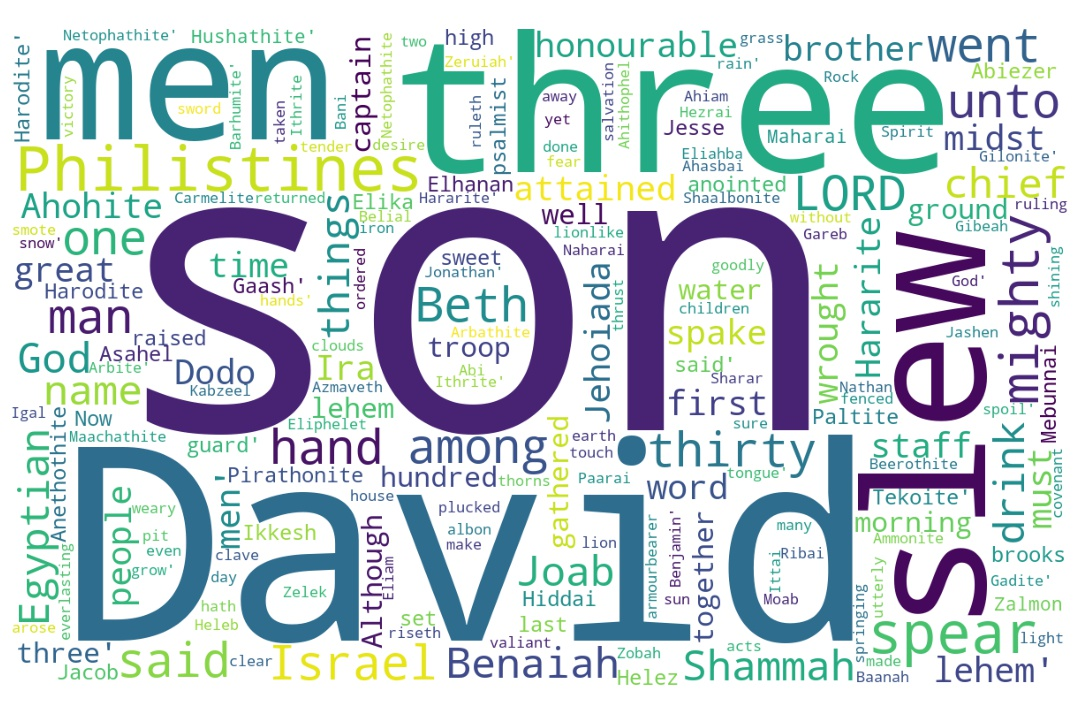
\includegraphics[width=\linewidth]{10OT-2Samuel/2Samuel23-WordCloud.jpg}
  \caption{1 Samuel 23 Word Cloud}
  \label{fig:1 Samuel 23 Word Cloud}
\end{figure}

%%%%%%%%%%%%%%%%%%%%%%%%%%%%%%%%%%%%%%%%%
%%%%%%%%%%%%%%%%%%%%%%%%%%%%%%%%%%%%%%%%%


\marginpar{\scriptsize \centering \fcolorbox{bone}{lime}{\textbf{DAVID"S MIGHTY MEN}}\\ (2 Samuel 23:1--39) 
\begin{compactenum}[I.][8]
    \item A Final  \textbf{Message} \index[scripture]{2Samuel!2Sa 22:01} (2Sa 22:1) 
    \item Things that are  \textbf{Memorable} \index[scripture]{2Samuel!2Sa 22:01} (2Sa 22:1) 
    \item The  \textbf{Mighty} Men \index[scripture]{2Samuel!2Sa 22:01} (2Sa 22:1) 
    \item Those Even  \textbf{More} Special \index[scripture]{2Samuel!2Sa 22:01} (2Sa 22:1) 
    \item A  \textbf{Moment} \index[scripture]{2Samuel!2Sa 23:13--17} (2Sa 23:13--17) 
    \item The  \textbf{Mistake} \index[scripture]{2Samuel!2Sa 23:39} (2Sa 23:39) 
   \item A  \textbf{Message} \index[scripture]{2Samuel!2Sa 23:13--17} (2Sa 23:13--17) 
\end{compactenum} }

\footnote{\textcolor[cmyk]{0.99998,1,0,0}{\hyperlink{TOC}{Return to end of Table of Contents.}}}\footnote{\href{https://audiobible.com/bible/2_samuel_23.html}{\textcolor[cmyk]{0.99998,1,0,0}{2 Samuel 23 Audio}}}\textcolor[cmyk]{0.99998,1,0,0}{Now these \emph{be} the last words of David. David the son of Jesse said, and the man \emph{who} \emph{was} raised up on high, the anointed of the God of Jacob, and the sweet psalmist of Israel, said,}
[2] \textcolor[cmyk]{0.99998,1,0,0}{The Spirit of the LORD spake by me, and his word \emph{was} in my tongue.}
[3] \textcolor[cmyk]{0.99998,1,0,0}{The God of Israel said, the Rock of Israel spake to me, He that ruleth over men \emph{must} \emph{be} just, ruling in the fear of God.}
[4] \textcolor[cmyk]{0.99998,1,0,0}{And \emph{he} \emph{shall} \emph{be} as the light of the morning, \emph{when} the sun riseth, \emph{even} \fcolorbox{bone}{bone}{a}morning without clouds; \emph{as} the tender grass \emph{springing} out of the earth by clear shining after rain.}
[5] \textcolor[cmyk]{0.99998,1,0,0}{Although my house \emph{be} not so with God; yet he hath made with me an everlasting covenant, ordered in all \emph{things}, and sure: for \emph{this} \emph{is} all my salvation, and all \emph{my} desire, although he make \emph{it} not to grow.}\\
\\
\P \textcolor[cmyk]{0.99998,1,0,0}{But \emph{the} \emph{sons} of Belial \emph{shall} \emph{be} all of them as thorns thrust away, because they cannot be taken with hands:}
[7] \textcolor[cmyk]{0.99998,1,0,0}{But the man \emph{that} shall touch them must be fenced with iron and the staff of \fcolorbox{bone}{bone}{a}spear; and they shall be utterly burned with fire in the \emph{same} place.}\\
\\
\P \textcolor[cmyk]{0.99998,1,0,0}{These \emph{be} the names of the mighty men whom David had: The Tachmonite that sat in the seat, chief among the captains; the same \emph{was} Adino the Eznite: \emph{he} \emph{lift} \emph{up} \emph{his} \emph{spear} against eight hundred, whom he slew at one time.}
[9] \textcolor[cmyk]{0.99998,1,0,0}{And after him \emph{was} Eleazar the son of Dodo the Ahohite, \emph{one} of the three mighty men with David, when they defied the Philistines \emph{that} were there gathered together to battle, and the men of Israel were gone away:}
[10] \textcolor[cmyk]{0.99998,1,0,0}{He arose, and smote the Philistines until his hand was weary, and his hand clave unto the sword: and the LORD wrought \fcolorbox{bone}{bone}{a}great victory that day; and the people returned after him only to spoil.}
[11] \textcolor[cmyk]{0.99998,1,0,0}{And after him \emph{was} Shammah the son of Agee the Hararite. And the Philistines were gathered together into \fcolorbox{bone}{bone}{a}troop, where was \fcolorbox{bone}{bone}{a}piece of ground full of lentiles: and the people fled from the Philistines.}
[12] \textcolor[cmyk]{0.99998,1,0,0}{But he stood in the midst of the ground, and defended it, and slew the Philistines: and the LORD wrought \fcolorbox{bone}{bone}{a}great victory.}
[13] \textcolor[cmyk]{0.99998,1,0,0}{And three of the thirty chief went down, and came to David in the harvest time unto the cave of Adullam: and the troop of the Philistines pitched in the valley of Rephaim.}
[14] \textcolor[cmyk]{0.99998,1,0,0}{And David \emph{was} then in an hold, and the garrison of the Philistines \emph{was} then \emph{in} Beth-lehem.}
[15] \textcolor[cmyk]{0.99998,1,0,0}{And David longed, and said, Oh that one would give me drink of the water of the well of Beth-lehem, which \emph{is} by the gate!}
[16] \textcolor[cmyk]{0.99998,1,0,0}{And the three mighty men brake through the host of the Philistines, and drew water out of the well of Beth-lehem, that \emph{was} by the gate, and took \emph{it}, and brought \emph{it} to David: nevertheless he would not drink thereof, but poured it out unto the LORD.}
[17] \textcolor[cmyk]{0.99998,1,0,0}{And he said, Be it far from me, O LORD, that I should do this: \emph{is} \emph{not} \emph{this} the blood of the men that went in jeopardy of their lives? therefore he would not drink it. These things did these three mighty men.}
[18] \textcolor[cmyk]{0.99998,1,0,0}{And Abishai, the brother of Joab, the son of Zeruiah, was chief among three. And he lifted up his spear against three hundred, \emph{and} slew \emph{them}, and had the name among three.}
[19] \textcolor[cmyk]{0.99998,1,0,0}{Was he not most honourable of three? therefore he was their captain: howbeit he attained not unto the \emph{first} three.}
[20] \textcolor[cmyk]{0.99998,1,0,0}{And Benaiah the son of Jehoiada, the son of \fcolorbox{bone}{bone}{a}valiant man, of Kabzeel, who had done many acts, he slew two lionlike men of Moab: he went down also and slew \fcolorbox{bone}{bone}{a}lion in the midst of \fcolorbox{bone}{bone}{a}pit in time of snow:}
[21] \textcolor[cmyk]{0.99998,1,0,0}{And he slew an Egyptian, \fcolorbox{bone}{bone}{a}goodly man: and the Egyptian had \fcolorbox{bone}{bone}{a}spear in his hand; but he went down to him with \fcolorbox{bone}{bone}{a}staff, and plucked the spear out of the Egyptian's hand, and slew him with his own spear.}
[22] \textcolor[cmyk]{0.99998,1,0,0}{These \emph{things} did Benaiah the son of Jehoiada, and had the name among three mighty men.}
[23] \textcolor[cmyk]{0.99998,1,0,0}{He was more honourable than the thirty, but he attained not to the \emph{first} three. And David set him over his guard.}
[24] \textcolor[cmyk]{0.99998,1,0,0}{Asahel the brother of Joab \emph{was} one of the thirty; Elhanan the son of Dodo of Beth-lehem,}
[25] \textcolor[cmyk]{0.99998,1,0,0}{Shammah the Harodite, Elika the Harodite,}
[26] \textcolor[cmyk]{0.99998,1,0,0}{Helez the Paltite, Ira the son of Ikkesh the Tekoite,}
[27] \textcolor[cmyk]{0.99998,1,0,0}{Abiezer the Anethothite, Mebunnai the Hushathite,}
[28] \textcolor[cmyk]{0.99998,1,0,0}{Zalmon the Ahohite, Maharai the Netophathite,}
[29] \textcolor[cmyk]{0.99998,1,0,0}{Heleb the son of Baanah, \fcolorbox{bone}{bone}{a}Netophathite, Ittai the son of Ribai out of Gibeah of the children of Benjamin,}
[30] \textcolor[cmyk]{0.99998,1,0,0}{Benaiah the Pirathonite, Hiddai of the brooks of Gaash,}
[31] \textcolor[cmyk]{0.99998,1,0,0}{Abi-albon the Arbathite, Azmaveth the Barhumite,}
[32] \textcolor[cmyk]{0.99998,1,0,0}{Eliahba the Shaalbonite, of the sons of Jashen, Jonathan,}
[33] \textcolor[cmyk]{0.99998,1,0,0}{Shammah the Hararite, Ahiam the son of Sharar the Hararite,}
[34] \textcolor[cmyk]{0.99998,1,0,0}{Eliphelet the son of Ahasbai, the son of the Maachathite, Eliam the son of Ahithophel the Gilonite,}
[35] \textcolor[cmyk]{0.99998,1,0,0}{Hezrai the Carmelite, Paarai the Arbite,}
[36] \textcolor[cmyk]{0.99998,1,0,0}{Igal the son of Nathan of Zobah, Bani the Gadite,}
[37] \textcolor[cmyk]{0.99998,1,0,0}{Zelek the Ammonite, Naharai the Beerothite, armourbearer to Joab the son of Zeruiah,}
[38] \textcolor[cmyk]{0.99998,1,0,0}{Ira an Ithrite, Gareb an Ithrite,}
[39] \textcolor[cmyk]{0.99998,1,0,0}{Uriah the Hittite: thirty and seven in all.}
\index[NWIV]{37!2Samuel!2Sa 23:1}\index[AWIP]{Now!2Samuel!2Sa 23:1}\index[AWIP]{these!2Samuel!2Sa 23:1}\index[AWIP]{\emph{be}!2Samuel!2Sa 23:1}\index[AWIP]{the!2Samuel!2Sa 23:1}\index[AWIP]{the!2Samuel!2Sa 23:1 (2)}\index[AWIP]{the!2Samuel!2Sa 23:1 (3)}\index[AWIP]{the!2Samuel!2Sa 23:1 (4)}\index[AWIP]{the!2Samuel!2Sa 23:1 (5)}\index[AWIP]{the!2Samuel!2Sa 23:1 (6)}\index[AWIP]{last!2Samuel!2Sa 23:1}\index[AWIP]{words!2Samuel!2Sa 23:1}\index[AWIP]{of!2Samuel!2Sa 23:1}\index[AWIP]{of!2Samuel!2Sa 23:1 (2)}\index[AWIP]{of!2Samuel!2Sa 23:1 (3)}\index[AWIP]{of!2Samuel!2Sa 23:1 (4)}\index[AWIP]{of!2Samuel!2Sa 23:1 (5)}\index[AWIP]{David!2Samuel!2Sa 23:1}\index[AWIP]{David!2Samuel!2Sa 23:1 (2)}\index[AWIP]{son!2Samuel!2Sa 23:1}\index[AWIP]{Jesse!2Samuel!2Sa 23:1}\index[AWIP]{said!2Samuel!2Sa 23:1}\index[AWIP]{said!2Samuel!2Sa 23:1 (2)}\index[AWIP]{and!2Samuel!2Sa 23:1}\index[AWIP]{and!2Samuel!2Sa 23:1 (2)}\index[AWIP]{man!2Samuel!2Sa 23:1}\index[AWIP]{\emph{who}!2Samuel!2Sa 23:1}\index[AWIP]{\emph{was}!2Samuel!2Sa 23:1}\index[AWIP]{raised!2Samuel!2Sa 23:1}\index[AWIP]{up!2Samuel!2Sa 23:1}\index[AWIP]{on!2Samuel!2Sa 23:1}\index[AWIP]{high!2Samuel!2Sa 23:1}\index[AWIP]{anointed!2Samuel!2Sa 23:1}\index[AWIP]{God!2Samuel!2Sa 23:1}\index[AWIP]{Jacob!2Samuel!2Sa 23:1}\index[AWIP]{sweet!2Samuel!2Sa 23:1}\index[AWIP]{psalmist!2Samuel!2Sa 23:1}\index[AWIP]{Israel!2Samuel!2Sa 23:1}\index[AWIP]{\emph{be}!2Samuel!2Sa 23:1}\index[AWIP]{\emph{who}!2Samuel!2Sa 23:1}\index[AWIP]{\emph{was}!2Samuel!2Sa 23:1}

\index[NWIV]{15!2Samuel!2Sa 23:2}\index[AWIP]{The!2Samuel!2Sa 23:2}\index[AWIP]{Spirit!2Samuel!2Sa 23:2}\index[AWIP]{of!2Samuel!2Sa 23:2}\index[AWIP]{the!2Samuel!2Sa 23:2}\index[AWIP]{LORD!2Samuel!2Sa 23:2}\index[AWIP]{spake!2Samuel!2Sa 23:2}\index[AWIP]{by!2Samuel!2Sa 23:2}\index[AWIP]{me!2Samuel!2Sa 23:2}\index[AWIP]{and!2Samuel!2Sa 23:2}\index[AWIP]{his!2Samuel!2Sa 23:2}\index[AWIP]{word!2Samuel!2Sa 23:2}\index[AWIP]{\emph{was}!2Samuel!2Sa 23:2}\index[AWIP]{in!2Samuel!2Sa 23:2}\index[AWIP]{my!2Samuel!2Sa 23:2}\index[AWIP]{tongue!2Samuel!2Sa 23:2}\index[AWIP]{\emph{was}!2Samuel!2Sa 23:2}

\index[NWIV]{26!2Samuel!2Sa 23:3}\index[AWIP]{The!2Samuel!2Sa 23:3}\index[AWIP]{God!2Samuel!2Sa 23:3}\index[AWIP]{God!2Samuel!2Sa 23:3 (2)}\index[AWIP]{of!2Samuel!2Sa 23:3}\index[AWIP]{of!2Samuel!2Sa 23:3 (2)}\index[AWIP]{of!2Samuel!2Sa 23:3 (3)}\index[AWIP]{Israel!2Samuel!2Sa 23:3}\index[AWIP]{Israel!2Samuel!2Sa 23:3 (2)}\index[AWIP]{said!2Samuel!2Sa 23:3}\index[AWIP]{the!2Samuel!2Sa 23:3}\index[AWIP]{the!2Samuel!2Sa 23:3 (2)}\index[AWIP]{Rock!2Samuel!2Sa 23:3}\index[AWIP]{spake!2Samuel!2Sa 23:3}\index[AWIP]{to!2Samuel!2Sa 23:3}\index[AWIP]{me!2Samuel!2Sa 23:3}\index[AWIP]{He!2Samuel!2Sa 23:3}\index[AWIP]{that!2Samuel!2Sa 23:3}\index[AWIP]{ruleth!2Samuel!2Sa 23:3}\index[AWIP]{over!2Samuel!2Sa 23:3}\index[AWIP]{men!2Samuel!2Sa 23:3}\index[AWIP]{\emph{must}!2Samuel!2Sa 23:3}\index[AWIP]{\emph{be}!2Samuel!2Sa 23:3}\index[AWIP]{just!2Samuel!2Sa 23:3}\index[AWIP]{ruling!2Samuel!2Sa 23:3}\index[AWIP]{in!2Samuel!2Sa 23:3}\index[AWIP]{fear!2Samuel!2Sa 23:3}\index[AWIP]{\emph{must}!2Samuel!2Sa 23:3}\index[AWIP]{\emph{be}!2Samuel!2Sa 23:3}

\index[NWIV]{33!2Samuel!2Sa 23:4}\index[AWIP]{And!2Samuel!2Sa 23:4}\index[AWIP]{\emph{he}!2Samuel!2Sa 23:4}\index[AWIP]{\emph{shall}!2Samuel!2Sa 23:4}\index[AWIP]{\emph{be}!2Samuel!2Sa 23:4}\index[AWIP]{as!2Samuel!2Sa 23:4}\index[AWIP]{the!2Samuel!2Sa 23:4}\index[AWIP]{the!2Samuel!2Sa 23:4 (2)}\index[AWIP]{the!2Samuel!2Sa 23:4 (3)}\index[AWIP]{the!2Samuel!2Sa 23:4 (4)}\index[AWIP]{the!2Samuel!2Sa 23:4 (5)}\index[AWIP]{light!2Samuel!2Sa 23:4}\index[AWIP]{of!2Samuel!2Sa 23:4}\index[AWIP]{of!2Samuel!2Sa 23:4 (2)}\index[AWIP]{morning!2Samuel!2Sa 23:4}\index[AWIP]{morning!2Samuel!2Sa 23:4 (2)}\index[AWIP]{\emph{when}!2Samuel!2Sa 23:4}\index[AWIP]{sun!2Samuel!2Sa 23:4}\index[AWIP]{riseth!2Samuel!2Sa 23:4}\index[AWIP]{\emph{even}!2Samuel!2Sa 23:4}\index[AWIP]{a!2Samuel!2Sa 23:4}\index[AWIP]{without!2Samuel!2Sa 23:4}\index[AWIP]{clouds!2Samuel!2Sa 23:4}\index[AWIP]{\emph{as}!2Samuel!2Sa 23:4}\index[AWIP]{tender!2Samuel!2Sa 23:4}\index[AWIP]{grass!2Samuel!2Sa 23:4}\index[AWIP]{\emph{springing}!2Samuel!2Sa 23:4}\index[AWIP]{out!2Samuel!2Sa 23:4}\index[AWIP]{earth!2Samuel!2Sa 23:4}\index[AWIP]{by!2Samuel!2Sa 23:4}\index[AWIP]{clear!2Samuel!2Sa 23:4}\index[AWIP]{shining!2Samuel!2Sa 23:4}\index[AWIP]{after!2Samuel!2Sa 23:4}\index[AWIP]{rain!2Samuel!2Sa 23:4}\index[AWIP]{\emph{he}!2Samuel!2Sa 23:4}\index[AWIP]{\emph{shall}!2Samuel!2Sa 23:4}\index[AWIP]{\emph{be}!2Samuel!2Sa 23:4}\index[AWIP]{\emph{when}!2Samuel!2Sa 23:4}\index[AWIP]{\emph{even}!2Samuel!2Sa 23:4}\index[AWIP]{\emph{as}!2Samuel!2Sa 23:4}\index[AWIP]{\emph{springing}!2Samuel!2Sa 23:4}

\index[NWIV]{40!2Samuel!2Sa 23:5}\index[AWIP]{Although!2Samuel!2Sa 23:5}\index[AWIP]{my!2Samuel!2Sa 23:5}\index[AWIP]{my!2Samuel!2Sa 23:5 (2)}\index[AWIP]{house!2Samuel!2Sa 23:5}\index[AWIP]{\emph{be}!2Samuel!2Sa 23:5}\index[AWIP]{not!2Samuel!2Sa 23:5}\index[AWIP]{not!2Samuel!2Sa 23:5 (2)}\index[AWIP]{so!2Samuel!2Sa 23:5}\index[AWIP]{with!2Samuel!2Sa 23:5}\index[AWIP]{with!2Samuel!2Sa 23:5 (2)}\index[AWIP]{God!2Samuel!2Sa 23:5}\index[AWIP]{yet!2Samuel!2Sa 23:5}\index[AWIP]{he!2Samuel!2Sa 23:5}\index[AWIP]{he!2Samuel!2Sa 23:5 (2)}\index[AWIP]{hath!2Samuel!2Sa 23:5}\index[AWIP]{made!2Samuel!2Sa 23:5}\index[AWIP]{me!2Samuel!2Sa 23:5}\index[AWIP]{an!2Samuel!2Sa 23:5}\index[AWIP]{everlasting!2Samuel!2Sa 23:5}\index[AWIP]{covenant!2Samuel!2Sa 23:5}\index[AWIP]{ordered!2Samuel!2Sa 23:5}\index[AWIP]{in!2Samuel!2Sa 23:5}\index[AWIP]{all!2Samuel!2Sa 23:5}\index[AWIP]{all!2Samuel!2Sa 23:5 (2)}\index[AWIP]{all!2Samuel!2Sa 23:5 (3)}\index[AWIP]{\emph{things}!2Samuel!2Sa 23:5}\index[AWIP]{and!2Samuel!2Sa 23:5}\index[AWIP]{and!2Samuel!2Sa 23:5 (2)}\index[AWIP]{sure!2Samuel!2Sa 23:5}\index[AWIP]{for!2Samuel!2Sa 23:5}\index[AWIP]{\emph{this}!2Samuel!2Sa 23:5}\index[AWIP]{\emph{is}!2Samuel!2Sa 23:5}\index[AWIP]{salvation!2Samuel!2Sa 23:5}\index[AWIP]{\emph{my}!2Samuel!2Sa 23:5}\index[AWIP]{desire!2Samuel!2Sa 23:5}\index[AWIP]{although!2Samuel!2Sa 23:5}\index[AWIP]{make!2Samuel!2Sa 23:5}\index[AWIP]{\emph{it}!2Samuel!2Sa 23:5}\index[AWIP]{to!2Samuel!2Sa 23:5}\index[AWIP]{grow!2Samuel!2Sa 23:5}\index[AWIP]{\emph{be}!2Samuel!2Sa 23:5}\index[AWIP]{\emph{things}!2Samuel!2Sa 23:5}\index[AWIP]{\emph{this}!2Samuel!2Sa 23:5}\index[AWIP]{\emph{is}!2Samuel!2Sa 23:5}\index[AWIP]{\emph{my}!2Samuel!2Sa 23:5}\index[AWIP]{\emph{it}!2Samuel!2Sa 23:5}

\index[NWIV]{21!2Samuel!2Sa 23:6}\index[AWIP]{But!2Samuel!2Sa 23:6}\index[AWIP]{\emph{the}!2Samuel!2Sa 23:6}\index[AWIP]{\emph{sons}!2Samuel!2Sa 23:6}\index[AWIP]{of!2Samuel!2Sa 23:6}\index[AWIP]{of!2Samuel!2Sa 23:6 (2)}\index[AWIP]{Belial!2Samuel!2Sa 23:6}\index[AWIP]{\emph{shall}!2Samuel!2Sa 23:6}\index[AWIP]{\emph{be}!2Samuel!2Sa 23:6}\index[AWIP]{all!2Samuel!2Sa 23:6}\index[AWIP]{them!2Samuel!2Sa 23:6}\index[AWIP]{as!2Samuel!2Sa 23:6}\index[AWIP]{thorns!2Samuel!2Sa 23:6}\index[AWIP]{thrust!2Samuel!2Sa 23:6}\index[AWIP]{away!2Samuel!2Sa 23:6}\index[AWIP]{because!2Samuel!2Sa 23:6}\index[AWIP]{they!2Samuel!2Sa 23:6}\index[AWIP]{cannot!2Samuel!2Sa 23:6}\index[AWIP]{be!2Samuel!2Sa 23:6}\index[AWIP]{taken!2Samuel!2Sa 23:6}\index[AWIP]{with!2Samuel!2Sa 23:6}\index[AWIP]{hands!2Samuel!2Sa 23:6}\index[AWIP]{\emph{the}!2Samuel!2Sa 23:6}\index[AWIP]{\emph{sons}!2Samuel!2Sa 23:6}\index[AWIP]{\emph{shall}!2Samuel!2Sa 23:6}\index[AWIP]{\emph{be}!2Samuel!2Sa 23:6}

\index[NWIV]{30!2Samuel!2Sa 23:7}\index[AWIP]{But!2Samuel!2Sa 23:7}\index[AWIP]{the!2Samuel!2Sa 23:7}\index[AWIP]{the!2Samuel!2Sa 23:7 (2)}\index[AWIP]{the!2Samuel!2Sa 23:7 (3)}\index[AWIP]{man!2Samuel!2Sa 23:7}\index[AWIP]{\emph{that}!2Samuel!2Sa 23:7}\index[AWIP]{shall!2Samuel!2Sa 23:7}\index[AWIP]{shall!2Samuel!2Sa 23:7 (2)}\index[AWIP]{touch!2Samuel!2Sa 23:7}\index[AWIP]{them!2Samuel!2Sa 23:7}\index[AWIP]{must!2Samuel!2Sa 23:7}\index[AWIP]{be!2Samuel!2Sa 23:7}\index[AWIP]{be!2Samuel!2Sa 23:7 (2)}\index[AWIP]{fenced!2Samuel!2Sa 23:7}\index[AWIP]{with!2Samuel!2Sa 23:7}\index[AWIP]{with!2Samuel!2Sa 23:7 (2)}\index[AWIP]{iron!2Samuel!2Sa 23:7}\index[AWIP]{and!2Samuel!2Sa 23:7}\index[AWIP]{and!2Samuel!2Sa 23:7 (2)}\index[AWIP]{staff!2Samuel!2Sa 23:7}\index[AWIP]{of!2Samuel!2Sa 23:7}\index[AWIP]{a!2Samuel!2Sa 23:7}\index[AWIP]{spear!2Samuel!2Sa 23:7}\index[AWIP]{they!2Samuel!2Sa 23:7}\index[AWIP]{utterly!2Samuel!2Sa 23:7}\index[AWIP]{burned!2Samuel!2Sa 23:7}\index[AWIP]{fire!2Samuel!2Sa 23:7}\index[AWIP]{in!2Samuel!2Sa 23:7}\index[AWIP]{\emph{same}!2Samuel!2Sa 23:7}\index[AWIP]{place!2Samuel!2Sa 23:7}\index[AWIP]{\emph{that}!2Samuel!2Sa 23:7}\index[AWIP]{\emph{same}!2Samuel!2Sa 23:7}

\index[NWIV]{42!2Samuel!2Sa 23:8}\index[AWIP]{These!2Samuel!2Sa 23:8}\index[AWIP]{\emph{be}!2Samuel!2Sa 23:8}\index[AWIP]{the!2Samuel!2Sa 23:8}\index[AWIP]{the!2Samuel!2Sa 23:8 (2)}\index[AWIP]{the!2Samuel!2Sa 23:8 (3)}\index[AWIP]{the!2Samuel!2Sa 23:8 (4)}\index[AWIP]{the!2Samuel!2Sa 23:8 (5)}\index[AWIP]{the!2Samuel!2Sa 23:8 (6)}\index[AWIP]{names!2Samuel!2Sa 23:8}\index[AWIP]{of!2Samuel!2Sa 23:8}\index[AWIP]{mighty!2Samuel!2Sa 23:8}\index[AWIP]{men!2Samuel!2Sa 23:8}\index[AWIP]{whom!2Samuel!2Sa 23:8}\index[AWIP]{whom!2Samuel!2Sa 23:8 (2)}\index[AWIP]{David!2Samuel!2Sa 23:8}\index[AWIP]{had!2Samuel!2Sa 23:8}\index[AWIP]{The!2Samuel!2Sa 23:8}\index[AWIP]{Tachmonite!2Samuel!2Sa 23:8}\index[AWIP]{that!2Samuel!2Sa 23:8}\index[AWIP]{sat!2Samuel!2Sa 23:8}\index[AWIP]{in!2Samuel!2Sa 23:8}\index[AWIP]{seat!2Samuel!2Sa 23:8}\index[AWIP]{chief!2Samuel!2Sa 23:8}\index[AWIP]{among!2Samuel!2Sa 23:8}\index[AWIP]{captains!2Samuel!2Sa 23:8}\index[AWIP]{same!2Samuel!2Sa 23:8}\index[AWIP]{\emph{was}!2Samuel!2Sa 23:8}\index[AWIP]{Adino!2Samuel!2Sa 23:8}\index[AWIP]{Eznite!2Samuel!2Sa 23:8}\index[AWIP]{\emph{he}!2Samuel!2Sa 23:8}\index[AWIP]{\emph{lift}!2Samuel!2Sa 23:8}\index[AWIP]{\emph{up}!2Samuel!2Sa 23:8}\index[AWIP]{\emph{his}!2Samuel!2Sa 23:8}\index[AWIP]{\emph{spear}!2Samuel!2Sa 23:8}\index[AWIP]{against!2Samuel!2Sa 23:8}\index[AWIP]{eight!2Samuel!2Sa 23:8}\index[AWIP]{hundred!2Samuel!2Sa 23:8}\index[AWIP]{he!2Samuel!2Sa 23:8}\index[AWIP]{slew!2Samuel!2Sa 23:8}\index[AWIP]{at!2Samuel!2Sa 23:8}\index[AWIP]{one!2Samuel!2Sa 23:8}\index[AWIP]{time!2Samuel!2Sa 23:8}\index[AWIP]{\emph{be}!2Samuel!2Sa 23:8}\index[AWIP]{\emph{was}!2Samuel!2Sa 23:8}\index[AWIP]{\emph{he}!2Samuel!2Sa 23:8}\index[AWIP]{\emph{lift}!2Samuel!2Sa 23:8}\index[AWIP]{\emph{up}!2Samuel!2Sa 23:8}\index[AWIP]{\emph{his}!2Samuel!2Sa 23:8}\index[AWIP]{\emph{spear}!2Samuel!2Sa 23:8}

\index[NWIV]{39!2Samuel!2Sa 23:9}\index[AWIP]{And!2Samuel!2Sa 23:9}\index[AWIP]{after!2Samuel!2Sa 23:9}\index[AWIP]{him!2Samuel!2Sa 23:9}\index[AWIP]{\emph{was}!2Samuel!2Sa 23:9}\index[AWIP]{Eleazar!2Samuel!2Sa 23:9}\index[AWIP]{the!2Samuel!2Sa 23:9}\index[AWIP]{the!2Samuel!2Sa 23:9 (2)}\index[AWIP]{the!2Samuel!2Sa 23:9 (3)}\index[AWIP]{the!2Samuel!2Sa 23:9 (4)}\index[AWIP]{the!2Samuel!2Sa 23:9 (5)}\index[AWIP]{son!2Samuel!2Sa 23:9}\index[AWIP]{of!2Samuel!2Sa 23:9}\index[AWIP]{of!2Samuel!2Sa 23:9 (2)}\index[AWIP]{of!2Samuel!2Sa 23:9 (3)}\index[AWIP]{Dodo!2Samuel!2Sa 23:9}\index[AWIP]{Ahohite!2Samuel!2Sa 23:9}\index[AWIP]{\emph{one}!2Samuel!2Sa 23:9}\index[AWIP]{three!2Samuel!2Sa 23:9}\index[AWIP]{mighty!2Samuel!2Sa 23:9}\index[AWIP]{men!2Samuel!2Sa 23:9}\index[AWIP]{men!2Samuel!2Sa 23:9 (2)}\index[AWIP]{with!2Samuel!2Sa 23:9}\index[AWIP]{David!2Samuel!2Sa 23:9}\index[AWIP]{when!2Samuel!2Sa 23:9}\index[AWIP]{they!2Samuel!2Sa 23:9}\index[AWIP]{defied!2Samuel!2Sa 23:9}\index[AWIP]{Philistines!2Samuel!2Sa 23:9}\index[AWIP]{\emph{that}!2Samuel!2Sa 23:9}\index[AWIP]{were!2Samuel!2Sa 23:9}\index[AWIP]{were!2Samuel!2Sa 23:9 (2)}\index[AWIP]{there!2Samuel!2Sa 23:9}\index[AWIP]{gathered!2Samuel!2Sa 23:9}\index[AWIP]{together!2Samuel!2Sa 23:9}\index[AWIP]{to!2Samuel!2Sa 23:9}\index[AWIP]{battle!2Samuel!2Sa 23:9}\index[AWIP]{and!2Samuel!2Sa 23:9}\index[AWIP]{Israel!2Samuel!2Sa 23:9}\index[AWIP]{gone!2Samuel!2Sa 23:9}\index[AWIP]{away!2Samuel!2Sa 23:9}\index[AWIP]{\emph{was}!2Samuel!2Sa 23:9}\index[AWIP]{\emph{one}!2Samuel!2Sa 23:9}\index[AWIP]{\emph{that}!2Samuel!2Sa 23:9}

\index[NWIV]{36!2Samuel!2Sa 23:10}\index[AWIP]{He!2Samuel!2Sa 23:10}\index[AWIP]{arose!2Samuel!2Sa 23:10}\index[AWIP]{and!2Samuel!2Sa 23:10}\index[AWIP]{and!2Samuel!2Sa 23:10 (2)}\index[AWIP]{and!2Samuel!2Sa 23:10 (3)}\index[AWIP]{and!2Samuel!2Sa 23:10 (4)}\index[AWIP]{smote!2Samuel!2Sa 23:10}\index[AWIP]{the!2Samuel!2Sa 23:10}\index[AWIP]{the!2Samuel!2Sa 23:10 (2)}\index[AWIP]{the!2Samuel!2Sa 23:10 (3)}\index[AWIP]{the!2Samuel!2Sa 23:10 (4)}\index[AWIP]{Philistines!2Samuel!2Sa 23:10}\index[AWIP]{until!2Samuel!2Sa 23:10}\index[AWIP]{his!2Samuel!2Sa 23:10}\index[AWIP]{his!2Samuel!2Sa 23:10 (2)}\index[AWIP]{hand!2Samuel!2Sa 23:10}\index[AWIP]{hand!2Samuel!2Sa 23:10 (2)}\index[AWIP]{was!2Samuel!2Sa 23:10}\index[AWIP]{weary!2Samuel!2Sa 23:10}\index[AWIP]{clave!2Samuel!2Sa 23:10}\index[AWIP]{unto!2Samuel!2Sa 23:10}\index[AWIP]{sword!2Samuel!2Sa 23:10}\index[AWIP]{LORD!2Samuel!2Sa 23:10}\index[AWIP]{wrought!2Samuel!2Sa 23:10}\index[AWIP]{a!2Samuel!2Sa 23:10}\index[AWIP]{great!2Samuel!2Sa 23:10}\index[AWIP]{victory!2Samuel!2Sa 23:10}\index[AWIP]{that!2Samuel!2Sa 23:10}\index[AWIP]{day!2Samuel!2Sa 23:10}\index[AWIP]{people!2Samuel!2Sa 23:10}\index[AWIP]{returned!2Samuel!2Sa 23:10}\index[AWIP]{after!2Samuel!2Sa 23:10}\index[AWIP]{him!2Samuel!2Sa 23:10}\index[AWIP]{only!2Samuel!2Sa 23:10}\index[AWIP]{to!2Samuel!2Sa 23:10}\index[AWIP]{spoil!2Samuel!2Sa 23:10}

\index[NWIV]{36!2Samuel!2Sa 23:11}\index[AWIP]{And!2Samuel!2Sa 23:11}\index[AWIP]{And!2Samuel!2Sa 23:11 (2)}\index[AWIP]{after!2Samuel!2Sa 23:11}\index[AWIP]{him!2Samuel!2Sa 23:11}\index[AWIP]{\emph{was}!2Samuel!2Sa 23:11}\index[AWIP]{Shammah!2Samuel!2Sa 23:11}\index[AWIP]{the!2Samuel!2Sa 23:11}\index[AWIP]{the!2Samuel!2Sa 23:11 (2)}\index[AWIP]{the!2Samuel!2Sa 23:11 (3)}\index[AWIP]{the!2Samuel!2Sa 23:11 (4)}\index[AWIP]{the!2Samuel!2Sa 23:11 (5)}\index[AWIP]{son!2Samuel!2Sa 23:11}\index[AWIP]{of!2Samuel!2Sa 23:11}\index[AWIP]{of!2Samuel!2Sa 23:11 (2)}\index[AWIP]{of!2Samuel!2Sa 23:11 (3)}\index[AWIP]{Agee!2Samuel!2Sa 23:11}\index[AWIP]{Hararite!2Samuel!2Sa 23:11}\index[AWIP]{Philistines!2Samuel!2Sa 23:11}\index[AWIP]{Philistines!2Samuel!2Sa 23:11 (2)}\index[AWIP]{were!2Samuel!2Sa 23:11}\index[AWIP]{gathered!2Samuel!2Sa 23:11}\index[AWIP]{together!2Samuel!2Sa 23:11}\index[AWIP]{into!2Samuel!2Sa 23:11}\index[AWIP]{a!2Samuel!2Sa 23:11}\index[AWIP]{a!2Samuel!2Sa 23:11 (2)}\index[AWIP]{troop!2Samuel!2Sa 23:11}\index[AWIP]{where!2Samuel!2Sa 23:11}\index[AWIP]{was!2Samuel!2Sa 23:11}\index[AWIP]{piece!2Samuel!2Sa 23:11}\index[AWIP]{ground!2Samuel!2Sa 23:11}\index[AWIP]{full!2Samuel!2Sa 23:11}\index[AWIP]{lentiles!2Samuel!2Sa 23:11}\index[AWIP]{and!2Samuel!2Sa 23:11}\index[AWIP]{people!2Samuel!2Sa 23:11}\index[AWIP]{fled!2Samuel!2Sa 23:11}\index[AWIP]{from!2Samuel!2Sa 23:11}\index[AWIP]{\emph{was}!2Samuel!2Sa 23:11}

\index[NWIV]{23!2Samuel!2Sa 23:12}\index[AWIP]{But!2Samuel!2Sa 23:12}\index[AWIP]{he!2Samuel!2Sa 23:12}\index[AWIP]{stood!2Samuel!2Sa 23:12}\index[AWIP]{in!2Samuel!2Sa 23:12}\index[AWIP]{the!2Samuel!2Sa 23:12}\index[AWIP]{the!2Samuel!2Sa 23:12 (2)}\index[AWIP]{the!2Samuel!2Sa 23:12 (3)}\index[AWIP]{the!2Samuel!2Sa 23:12 (4)}\index[AWIP]{midst!2Samuel!2Sa 23:12}\index[AWIP]{of!2Samuel!2Sa 23:12}\index[AWIP]{ground!2Samuel!2Sa 23:12}\index[AWIP]{and!2Samuel!2Sa 23:12}\index[AWIP]{and!2Samuel!2Sa 23:12 (2)}\index[AWIP]{and!2Samuel!2Sa 23:12 (3)}\index[AWIP]{defended!2Samuel!2Sa 23:12}\index[AWIP]{it!2Samuel!2Sa 23:12}\index[AWIP]{slew!2Samuel!2Sa 23:12}\index[AWIP]{Philistines!2Samuel!2Sa 23:12}\index[AWIP]{LORD!2Samuel!2Sa 23:12}\index[AWIP]{wrought!2Samuel!2Sa 23:12}\index[AWIP]{a!2Samuel!2Sa 23:12}\index[AWIP]{great!2Samuel!2Sa 23:12}\index[AWIP]{victory!2Samuel!2Sa 23:12}

\index[NWIV]{33!2Samuel!2Sa 23:13}\index[AWIP]{And!2Samuel!2Sa 23:13}\index[AWIP]{three!2Samuel!2Sa 23:13}\index[AWIP]{of!2Samuel!2Sa 23:13}\index[AWIP]{of!2Samuel!2Sa 23:13 (2)}\index[AWIP]{of!2Samuel!2Sa 23:13 (3)}\index[AWIP]{of!2Samuel!2Sa 23:13 (4)}\index[AWIP]{the!2Samuel!2Sa 23:13}\index[AWIP]{the!2Samuel!2Sa 23:13 (2)}\index[AWIP]{the!2Samuel!2Sa 23:13 (3)}\index[AWIP]{the!2Samuel!2Sa 23:13 (4)}\index[AWIP]{the!2Samuel!2Sa 23:13 (5)}\index[AWIP]{the!2Samuel!2Sa 23:13 (6)}\index[AWIP]{thirty!2Samuel!2Sa 23:13}\index[AWIP]{chief!2Samuel!2Sa 23:13}\index[AWIP]{went!2Samuel!2Sa 23:13}\index[AWIP]{down!2Samuel!2Sa 23:13}\index[AWIP]{and!2Samuel!2Sa 23:13}\index[AWIP]{and!2Samuel!2Sa 23:13 (2)}\index[AWIP]{came!2Samuel!2Sa 23:13}\index[AWIP]{to!2Samuel!2Sa 23:13}\index[AWIP]{David!2Samuel!2Sa 23:13}\index[AWIP]{in!2Samuel!2Sa 23:13}\index[AWIP]{in!2Samuel!2Sa 23:13 (2)}\index[AWIP]{harvest!2Samuel!2Sa 23:13}\index[AWIP]{time!2Samuel!2Sa 23:13}\index[AWIP]{unto!2Samuel!2Sa 23:13}\index[AWIP]{cave!2Samuel!2Sa 23:13}\index[AWIP]{Adullam!2Samuel!2Sa 23:13}\index[AWIP]{troop!2Samuel!2Sa 23:13}\index[AWIP]{Philistines!2Samuel!2Sa 23:13}\index[AWIP]{pitched!2Samuel!2Sa 23:13}\index[AWIP]{valley!2Samuel!2Sa 23:13}\index[AWIP]{Rephaim!2Samuel!2Sa 23:13}

\index[NWIV]{17!2Samuel!2Sa 23:14}\index[AWIP]{And!2Samuel!2Sa 23:14}\index[AWIP]{David!2Samuel!2Sa 23:14}\index[AWIP]{\emph{was}!2Samuel!2Sa 23:14}\index[AWIP]{\emph{was}!2Samuel!2Sa 23:14 (2)}\index[AWIP]{then!2Samuel!2Sa 23:14}\index[AWIP]{then!2Samuel!2Sa 23:14 (2)}\index[AWIP]{in!2Samuel!2Sa 23:14}\index[AWIP]{an!2Samuel!2Sa 23:14}\index[AWIP]{hold!2Samuel!2Sa 23:14}\index[AWIP]{and!2Samuel!2Sa 23:14}\index[AWIP]{the!2Samuel!2Sa 23:14}\index[AWIP]{the!2Samuel!2Sa 23:14 (2)}\index[AWIP]{garrison!2Samuel!2Sa 23:14}\index[AWIP]{of!2Samuel!2Sa 23:14}\index[AWIP]{Philistines!2Samuel!2Sa 23:14}\index[AWIP]{\emph{in}!2Samuel!2Sa 23:14}\index[AWIP]{Beth-lehem!2Samuel!2Sa 23:14}\index[AWIP]{\emph{was}!2Samuel!2Sa 23:14}\index[AWIP]{\emph{was}!2Samuel!2Sa 23:14 (2)}\index[AWIP]{\emph{in}!2Samuel!2Sa 23:14}

\index[NWIV]{25!2Samuel!2Sa 23:15}\index[AWIP]{And!2Samuel!2Sa 23:15}\index[AWIP]{David!2Samuel!2Sa 23:15}\index[AWIP]{longed!2Samuel!2Sa 23:15}\index[AWIP]{and!2Samuel!2Sa 23:15}\index[AWIP]{said!2Samuel!2Sa 23:15}\index[AWIP]{Oh!2Samuel!2Sa 23:15}\index[AWIP]{that!2Samuel!2Sa 23:15}\index[AWIP]{one!2Samuel!2Sa 23:15}\index[AWIP]{would!2Samuel!2Sa 23:15}\index[AWIP]{give!2Samuel!2Sa 23:15}\index[AWIP]{me!2Samuel!2Sa 23:15}\index[AWIP]{drink!2Samuel!2Sa 23:15}\index[AWIP]{of!2Samuel!2Sa 23:15}\index[AWIP]{of!2Samuel!2Sa 23:15 (2)}\index[AWIP]{of!2Samuel!2Sa 23:15 (3)}\index[AWIP]{the!2Samuel!2Sa 23:15}\index[AWIP]{the!2Samuel!2Sa 23:15 (2)}\index[AWIP]{the!2Samuel!2Sa 23:15 (3)}\index[AWIP]{water!2Samuel!2Sa 23:15}\index[AWIP]{well!2Samuel!2Sa 23:15}\index[AWIP]{Beth-lehem!2Samuel!2Sa 23:15}\index[AWIP]{which!2Samuel!2Sa 23:15}\index[AWIP]{\emph{is}!2Samuel!2Sa 23:15}\index[AWIP]{by!2Samuel!2Sa 23:15}\index[AWIP]{gate!!2Samuel!2Sa 23:15}\index[AWIP]{\emph{is}!2Samuel!2Sa 23:15}

\index[NWIV]{47!2Samuel!2Sa 23:16}\index[AWIP]{And!2Samuel!2Sa 23:16}\index[AWIP]{the!2Samuel!2Sa 23:16}\index[AWIP]{the!2Samuel!2Sa 23:16 (2)}\index[AWIP]{the!2Samuel!2Sa 23:16 (3)}\index[AWIP]{the!2Samuel!2Sa 23:16 (4)}\index[AWIP]{the!2Samuel!2Sa 23:16 (5)}\index[AWIP]{the!2Samuel!2Sa 23:16 (6)}\index[AWIP]{three!2Samuel!2Sa 23:16}\index[AWIP]{mighty!2Samuel!2Sa 23:16}\index[AWIP]{men!2Samuel!2Sa 23:16}\index[AWIP]{brake!2Samuel!2Sa 23:16}\index[AWIP]{through!2Samuel!2Sa 23:16}\index[AWIP]{host!2Samuel!2Sa 23:16}\index[AWIP]{of!2Samuel!2Sa 23:16}\index[AWIP]{of!2Samuel!2Sa 23:16 (2)}\index[AWIP]{of!2Samuel!2Sa 23:16 (3)}\index[AWIP]{Philistines!2Samuel!2Sa 23:16}\index[AWIP]{and!2Samuel!2Sa 23:16}\index[AWIP]{and!2Samuel!2Sa 23:16 (2)}\index[AWIP]{and!2Samuel!2Sa 23:16 (3)}\index[AWIP]{drew!2Samuel!2Sa 23:16}\index[AWIP]{water!2Samuel!2Sa 23:16}\index[AWIP]{out!2Samuel!2Sa 23:16}\index[AWIP]{out!2Samuel!2Sa 23:16 (2)}\index[AWIP]{well!2Samuel!2Sa 23:16}\index[AWIP]{Beth-lehem!2Samuel!2Sa 23:16}\index[AWIP]{that!2Samuel!2Sa 23:16}\index[AWIP]{\emph{was}!2Samuel!2Sa 23:16}\index[AWIP]{by!2Samuel!2Sa 23:16}\index[AWIP]{gate!2Samuel!2Sa 23:16}\index[AWIP]{took!2Samuel!2Sa 23:16}\index[AWIP]{\emph{it}!2Samuel!2Sa 23:16}\index[AWIP]{\emph{it}!2Samuel!2Sa 23:16 (2)}\index[AWIP]{brought!2Samuel!2Sa 23:16}\index[AWIP]{to!2Samuel!2Sa 23:16}\index[AWIP]{David!2Samuel!2Sa 23:16}\index[AWIP]{nevertheless!2Samuel!2Sa 23:16}\index[AWIP]{he!2Samuel!2Sa 23:16}\index[AWIP]{would!2Samuel!2Sa 23:16}\index[AWIP]{not!2Samuel!2Sa 23:16}\index[AWIP]{drink!2Samuel!2Sa 23:16}\index[AWIP]{thereof!2Samuel!2Sa 23:16}\index[AWIP]{but!2Samuel!2Sa 23:16}\index[AWIP]{poured!2Samuel!2Sa 23:16}\index[AWIP]{it!2Samuel!2Sa 23:16}\index[AWIP]{unto!2Samuel!2Sa 23:16}\index[AWIP]{LORD!2Samuel!2Sa 23:16}\index[AWIP]{\emph{was}!2Samuel!2Sa 23:16}\index[AWIP]{\emph{it}!2Samuel!2Sa 23:16}\index[AWIP]{\emph{it}!2Samuel!2Sa 23:16 (2)}

\index[NWIV]{43!2Samuel!2Sa 23:17}\index[AWIP]{And!2Samuel!2Sa 23:17}\index[AWIP]{he!2Samuel!2Sa 23:17}\index[AWIP]{he!2Samuel!2Sa 23:17 (2)}\index[AWIP]{said!2Samuel!2Sa 23:17}\index[AWIP]{Be!2Samuel!2Sa 23:17}\index[AWIP]{it!2Samuel!2Sa 23:17}\index[AWIP]{it!2Samuel!2Sa 23:17 (2)}\index[AWIP]{far!2Samuel!2Sa 23:17}\index[AWIP]{from!2Samuel!2Sa 23:17}\index[AWIP]{me!2Samuel!2Sa 23:17}\index[AWIP]{O!2Samuel!2Sa 23:17}\index[AWIP]{LORD!2Samuel!2Sa 23:17}\index[AWIP]{that!2Samuel!2Sa 23:17}\index[AWIP]{that!2Samuel!2Sa 23:17 (2)}\index[AWIP]{I!2Samuel!2Sa 23:17}\index[AWIP]{should!2Samuel!2Sa 23:17}\index[AWIP]{do!2Samuel!2Sa 23:17}\index[AWIP]{this!2Samuel!2Sa 23:17}\index[AWIP]{\emph{is}!2Samuel!2Sa 23:17}\index[AWIP]{\emph{not}!2Samuel!2Sa 23:17}\index[AWIP]{\emph{this}!2Samuel!2Sa 23:17}\index[AWIP]{the!2Samuel!2Sa 23:17}\index[AWIP]{the!2Samuel!2Sa 23:17 (2)}\index[AWIP]{blood!2Samuel!2Sa 23:17}\index[AWIP]{of!2Samuel!2Sa 23:17}\index[AWIP]{of!2Samuel!2Sa 23:17 (2)}\index[AWIP]{men!2Samuel!2Sa 23:17}\index[AWIP]{men!2Samuel!2Sa 23:17 (2)}\index[AWIP]{went!2Samuel!2Sa 23:17}\index[AWIP]{in!2Samuel!2Sa 23:17}\index[AWIP]{jeopardy!2Samuel!2Sa 23:17}\index[AWIP]{their!2Samuel!2Sa 23:17}\index[AWIP]{lives?!2Samuel!2Sa 23:17}\index[AWIP]{therefore!2Samuel!2Sa 23:17}\index[AWIP]{would!2Samuel!2Sa 23:17}\index[AWIP]{not!2Samuel!2Sa 23:17}\index[AWIP]{drink!2Samuel!2Sa 23:17}\index[AWIP]{These!2Samuel!2Sa 23:17}\index[AWIP]{things!2Samuel!2Sa 23:17}\index[AWIP]{did!2Samuel!2Sa 23:17}\index[AWIP]{these!2Samuel!2Sa 23:17}\index[AWIP]{three!2Samuel!2Sa 23:17}\index[AWIP]{mighty!2Samuel!2Sa 23:17}\index[AWIP]{\emph{is}!2Samuel!2Sa 23:17}\index[AWIP]{\emph{not}!2Samuel!2Sa 23:17}\index[AWIP]{\emph{this}!2Samuel!2Sa 23:17}

\index[NWIV]{32!2Samuel!2Sa 23:18}\index[AWIP]{And!2Samuel!2Sa 23:18}\index[AWIP]{And!2Samuel!2Sa 23:18 (2)}\index[AWIP]{Abishai!2Samuel!2Sa 23:18}\index[AWIP]{the!2Samuel!2Sa 23:18}\index[AWIP]{the!2Samuel!2Sa 23:18 (2)}\index[AWIP]{the!2Samuel!2Sa 23:18 (3)}\index[AWIP]{brother!2Samuel!2Sa 23:18}\index[AWIP]{of!2Samuel!2Sa 23:18}\index[AWIP]{of!2Samuel!2Sa 23:18 (2)}\index[AWIP]{Joab!2Samuel!2Sa 23:18}\index[AWIP]{son!2Samuel!2Sa 23:18}\index[AWIP]{Zeruiah!2Samuel!2Sa 23:18}\index[AWIP]{was!2Samuel!2Sa 23:18}\index[AWIP]{chief!2Samuel!2Sa 23:18}\index[AWIP]{among!2Samuel!2Sa 23:18}\index[AWIP]{among!2Samuel!2Sa 23:18 (2)}\index[AWIP]{three!2Samuel!2Sa 23:18}\index[AWIP]{three!2Samuel!2Sa 23:18 (2)}\index[AWIP]{three!2Samuel!2Sa 23:18 (3)}\index[AWIP]{he!2Samuel!2Sa 23:18}\index[AWIP]{lifted!2Samuel!2Sa 23:18}\index[AWIP]{up!2Samuel!2Sa 23:18}\index[AWIP]{his!2Samuel!2Sa 23:18}\index[AWIP]{spear!2Samuel!2Sa 23:18}\index[AWIP]{against!2Samuel!2Sa 23:18}\index[AWIP]{hundred!2Samuel!2Sa 23:18}\index[AWIP]{\emph{and}!2Samuel!2Sa 23:18}\index[AWIP]{slew!2Samuel!2Sa 23:18}\index[AWIP]{\emph{them}!2Samuel!2Sa 23:18}\index[AWIP]{and!2Samuel!2Sa 23:18}\index[AWIP]{had!2Samuel!2Sa 23:18}\index[AWIP]{name!2Samuel!2Sa 23:18}\index[AWIP]{\emph{and}!2Samuel!2Sa 23:18}\index[AWIP]{\emph{them}!2Samuel!2Sa 23:18}

\index[NWIV]{20!2Samuel!2Sa 23:19}\index[AWIP]{Was!2Samuel!2Sa 23:19}\index[AWIP]{he!2Samuel!2Sa 23:19}\index[AWIP]{he!2Samuel!2Sa 23:19 (2)}\index[AWIP]{he!2Samuel!2Sa 23:19 (3)}\index[AWIP]{not!2Samuel!2Sa 23:19}\index[AWIP]{not!2Samuel!2Sa 23:19 (2)}\index[AWIP]{most!2Samuel!2Sa 23:19}\index[AWIP]{honourable!2Samuel!2Sa 23:19}\index[AWIP]{of!2Samuel!2Sa 23:19}\index[AWIP]{three?!2Samuel!2Sa 23:19}\index[AWIP]{therefore!2Samuel!2Sa 23:19}\index[AWIP]{was!2Samuel!2Sa 23:19}\index[AWIP]{their!2Samuel!2Sa 23:19}\index[AWIP]{captain!2Samuel!2Sa 23:19}\index[AWIP]{howbeit!2Samuel!2Sa 23:19}\index[AWIP]{attained!2Samuel!2Sa 23:19}\index[AWIP]{unto!2Samuel!2Sa 23:19}\index[AWIP]{the!2Samuel!2Sa 23:19}\index[AWIP]{\emph{first}!2Samuel!2Sa 23:19}\index[AWIP]{three!2Samuel!2Sa 23:19}\index[AWIP]{\emph{first}!2Samuel!2Sa 23:19}

\index[NWIV]{44!2Samuel!2Sa 23:20}\index[AWIP]{And!2Samuel!2Sa 23:20}\index[AWIP]{Benaiah!2Samuel!2Sa 23:20}\index[AWIP]{the!2Samuel!2Sa 23:20}\index[AWIP]{the!2Samuel!2Sa 23:20 (2)}\index[AWIP]{the!2Samuel!2Sa 23:20 (3)}\index[AWIP]{son!2Samuel!2Sa 23:20}\index[AWIP]{son!2Samuel!2Sa 23:20 (2)}\index[AWIP]{of!2Samuel!2Sa 23:20}\index[AWIP]{of!2Samuel!2Sa 23:20 (2)}\index[AWIP]{of!2Samuel!2Sa 23:20 (3)}\index[AWIP]{of!2Samuel!2Sa 23:20 (4)}\index[AWIP]{of!2Samuel!2Sa 23:20 (5)}\index[AWIP]{of!2Samuel!2Sa 23:20 (6)}\index[AWIP]{Jehoiada!2Samuel!2Sa 23:20}\index[AWIP]{a!2Samuel!2Sa 23:20}\index[AWIP]{a!2Samuel!2Sa 23:20 (2)}\index[AWIP]{a!2Samuel!2Sa 23:20 (3)}\index[AWIP]{valiant!2Samuel!2Sa 23:20}\index[AWIP]{man!2Samuel!2Sa 23:20}\index[AWIP]{Kabzeel!2Samuel!2Sa 23:20}\index[AWIP]{who!2Samuel!2Sa 23:20}\index[AWIP]{had!2Samuel!2Sa 23:20}\index[AWIP]{done!2Samuel!2Sa 23:20}\index[AWIP]{many!2Samuel!2Sa 23:20}\index[AWIP]{acts!2Samuel!2Sa 23:20}\index[AWIP]{he!2Samuel!2Sa 23:20}\index[AWIP]{he!2Samuel!2Sa 23:20 (2)}\index[AWIP]{slew!2Samuel!2Sa 23:20}\index[AWIP]{slew!2Samuel!2Sa 23:20 (2)}\index[AWIP]{two!2Samuel!2Sa 23:20}\index[AWIP]{lionlike!2Samuel!2Sa 23:20}\index[AWIP]{men!2Samuel!2Sa 23:20}\index[AWIP]{Moab!2Samuel!2Sa 23:20}\index[AWIP]{went!2Samuel!2Sa 23:20}\index[AWIP]{down!2Samuel!2Sa 23:20}\index[AWIP]{also!2Samuel!2Sa 23:20}\index[AWIP]{and!2Samuel!2Sa 23:20}\index[AWIP]{lion!2Samuel!2Sa 23:20}\index[AWIP]{in!2Samuel!2Sa 23:20}\index[AWIP]{in!2Samuel!2Sa 23:20 (2)}\index[AWIP]{midst!2Samuel!2Sa 23:20}\index[AWIP]{pit!2Samuel!2Sa 23:20}\index[AWIP]{time!2Samuel!2Sa 23:20}\index[AWIP]{snow!2Samuel!2Sa 23:20}

\index[NWIV]{42!2Samuel!2Sa 23:21}\index[AWIP]{And!2Samuel!2Sa 23:21}\index[AWIP]{he!2Samuel!2Sa 23:21}\index[AWIP]{he!2Samuel!2Sa 23:21 (2)}\index[AWIP]{slew!2Samuel!2Sa 23:21}\index[AWIP]{slew!2Samuel!2Sa 23:21 (2)}\index[AWIP]{an!2Samuel!2Sa 23:21}\index[AWIP]{Egyptian!2Samuel!2Sa 23:21}\index[AWIP]{Egyptian!2Samuel!2Sa 23:21 (2)}\index[AWIP]{a!2Samuel!2Sa 23:21}\index[AWIP]{a!2Samuel!2Sa 23:21 (2)}\index[AWIP]{a!2Samuel!2Sa 23:21 (3)}\index[AWIP]{goodly!2Samuel!2Sa 23:21}\index[AWIP]{man!2Samuel!2Sa 23:21}\index[AWIP]{and!2Samuel!2Sa 23:21}\index[AWIP]{and!2Samuel!2Sa 23:21 (2)}\index[AWIP]{and!2Samuel!2Sa 23:21 (3)}\index[AWIP]{the!2Samuel!2Sa 23:21}\index[AWIP]{the!2Samuel!2Sa 23:21 (2)}\index[AWIP]{the!2Samuel!2Sa 23:21 (3)}\index[AWIP]{had!2Samuel!2Sa 23:21}\index[AWIP]{spear!2Samuel!2Sa 23:21}\index[AWIP]{spear!2Samuel!2Sa 23:21 (2)}\index[AWIP]{spear!2Samuel!2Sa 23:21 (3)}\index[AWIP]{in!2Samuel!2Sa 23:21}\index[AWIP]{his!2Samuel!2Sa 23:21}\index[AWIP]{his!2Samuel!2Sa 23:21 (2)}\index[AWIP]{hand!2Samuel!2Sa 23:21}\index[AWIP]{hand!2Samuel!2Sa 23:21 (2)}\index[AWIP]{but!2Samuel!2Sa 23:21}\index[AWIP]{went!2Samuel!2Sa 23:21}\index[AWIP]{down!2Samuel!2Sa 23:21}\index[AWIP]{to!2Samuel!2Sa 23:21}\index[AWIP]{him!2Samuel!2Sa 23:21}\index[AWIP]{him!2Samuel!2Sa 23:21 (2)}\index[AWIP]{with!2Samuel!2Sa 23:21}\index[AWIP]{with!2Samuel!2Sa 23:21 (2)}\index[AWIP]{staff!2Samuel!2Sa 23:21}\index[AWIP]{plucked!2Samuel!2Sa 23:21}\index[AWIP]{out!2Samuel!2Sa 23:21}\index[AWIP]{of!2Samuel!2Sa 23:21}\index[AWIP]{Egyptian's!2Samuel!2Sa 23:21}\index[AWIP]{own!2Samuel!2Sa 23:21}

\index[NWIV]{16!2Samuel!2Sa 23:22}\index[AWIP]{These!2Samuel!2Sa 23:22}\index[AWIP]{\emph{things}!2Samuel!2Sa 23:22}\index[AWIP]{did!2Samuel!2Sa 23:22}\index[AWIP]{Benaiah!2Samuel!2Sa 23:22}\index[AWIP]{the!2Samuel!2Sa 23:22}\index[AWIP]{the!2Samuel!2Sa 23:22 (2)}\index[AWIP]{son!2Samuel!2Sa 23:22}\index[AWIP]{of!2Samuel!2Sa 23:22}\index[AWIP]{Jehoiada!2Samuel!2Sa 23:22}\index[AWIP]{and!2Samuel!2Sa 23:22}\index[AWIP]{had!2Samuel!2Sa 23:22}\index[AWIP]{name!2Samuel!2Sa 23:22}\index[AWIP]{among!2Samuel!2Sa 23:22}\index[AWIP]{three!2Samuel!2Sa 23:22}\index[AWIP]{mighty!2Samuel!2Sa 23:22}\index[AWIP]{men!2Samuel!2Sa 23:22}\index[AWIP]{\emph{things}!2Samuel!2Sa 23:22}

\index[NWIV]{22!2Samuel!2Sa 23:23}\index[AWIP]{He!2Samuel!2Sa 23:23}\index[AWIP]{was!2Samuel!2Sa 23:23}\index[AWIP]{more!2Samuel!2Sa 23:23}\index[AWIP]{honourable!2Samuel!2Sa 23:23}\index[AWIP]{than!2Samuel!2Sa 23:23}\index[AWIP]{the!2Samuel!2Sa 23:23}\index[AWIP]{the!2Samuel!2Sa 23:23 (2)}\index[AWIP]{thirty!2Samuel!2Sa 23:23}\index[AWIP]{but!2Samuel!2Sa 23:23}\index[AWIP]{he!2Samuel!2Sa 23:23}\index[AWIP]{attained!2Samuel!2Sa 23:23}\index[AWIP]{not!2Samuel!2Sa 23:23}\index[AWIP]{to!2Samuel!2Sa 23:23}\index[AWIP]{\emph{first}!2Samuel!2Sa 23:23}\index[AWIP]{three!2Samuel!2Sa 23:23}\index[AWIP]{And!2Samuel!2Sa 23:23}\index[AWIP]{David!2Samuel!2Sa 23:23}\index[AWIP]{set!2Samuel!2Sa 23:23}\index[AWIP]{him!2Samuel!2Sa 23:23}\index[AWIP]{over!2Samuel!2Sa 23:23}\index[AWIP]{his!2Samuel!2Sa 23:23}\index[AWIP]{guard!2Samuel!2Sa 23:23}\index[AWIP]{\emph{first}!2Samuel!2Sa 23:23}

\index[NWIV]{17!2Samuel!2Sa 23:24}\index[AWIP]{Asahel!2Samuel!2Sa 23:24}\index[AWIP]{the!2Samuel!2Sa 23:24}\index[AWIP]{the!2Samuel!2Sa 23:24 (2)}\index[AWIP]{the!2Samuel!2Sa 23:24 (3)}\index[AWIP]{brother!2Samuel!2Sa 23:24}\index[AWIP]{of!2Samuel!2Sa 23:24}\index[AWIP]{of!2Samuel!2Sa 23:24 (2)}\index[AWIP]{of!2Samuel!2Sa 23:24 (3)}\index[AWIP]{of!2Samuel!2Sa 23:24 (4)}\index[AWIP]{Joab!2Samuel!2Sa 23:24}\index[AWIP]{\emph{was}!2Samuel!2Sa 23:24}\index[AWIP]{one!2Samuel!2Sa 23:24}\index[AWIP]{thirty!2Samuel!2Sa 23:24}\index[AWIP]{Elhanan!2Samuel!2Sa 23:24}\index[AWIP]{son!2Samuel!2Sa 23:24}\index[AWIP]{Dodo!2Samuel!2Sa 23:24}\index[AWIP]{Beth-lehem!2Samuel!2Sa 23:24}\index[AWIP]{\emph{was}!2Samuel!2Sa 23:24}

\index[NWIV]{6!2Samuel!2Sa 23:25}\index[AWIP]{Shammah!2Samuel!2Sa 23:25}\index[AWIP]{the!2Samuel!2Sa 23:25}\index[AWIP]{the!2Samuel!2Sa 23:25 (2)}\index[AWIP]{Harodite!2Samuel!2Sa 23:25}\index[AWIP]{Harodite!2Samuel!2Sa 23:25 (2)}\index[AWIP]{Elika!2Samuel!2Sa 23:25}

\index[NWIV]{10!2Samuel!2Sa 23:26}\index[AWIP]{Helez!2Samuel!2Sa 23:26}\index[AWIP]{the!2Samuel!2Sa 23:26}\index[AWIP]{the!2Samuel!2Sa 23:26 (2)}\index[AWIP]{the!2Samuel!2Sa 23:26 (3)}\index[AWIP]{Paltite!2Samuel!2Sa 23:26}\index[AWIP]{Ira!2Samuel!2Sa 23:26}\index[AWIP]{son!2Samuel!2Sa 23:26}\index[AWIP]{of!2Samuel!2Sa 23:26}\index[AWIP]{Ikkesh!2Samuel!2Sa 23:26}\index[AWIP]{Tekoite!2Samuel!2Sa 23:26}

\index[NWIV]{6!2Samuel!2Sa 23:27}\index[AWIP]{Abiezer!2Samuel!2Sa 23:27}\index[AWIP]{the!2Samuel!2Sa 23:27}\index[AWIP]{the!2Samuel!2Sa 23:27 (2)}\index[AWIP]{Anethothite!2Samuel!2Sa 23:27}\index[AWIP]{Mebunnai!2Samuel!2Sa 23:27}\index[AWIP]{Hushathite!2Samuel!2Sa 23:27}

\index[NWIV]{6!2Samuel!2Sa 23:28}\index[AWIP]{Zalmon!2Samuel!2Sa 23:28}\index[AWIP]{the!2Samuel!2Sa 23:28}\index[AWIP]{the!2Samuel!2Sa 23:28 (2)}\index[AWIP]{Ahohite!2Samuel!2Sa 23:28}\index[AWIP]{Maharai!2Samuel!2Sa 23:28}\index[AWIP]{Netophathite!2Samuel!2Sa 23:28}

\index[NWIV]{20!2Samuel!2Sa 23:29}\index[AWIP]{Heleb!2Samuel!2Sa 23:29}\index[AWIP]{the!2Samuel!2Sa 23:29}\index[AWIP]{the!2Samuel!2Sa 23:29 (2)}\index[AWIP]{the!2Samuel!2Sa 23:29 (3)}\index[AWIP]{son!2Samuel!2Sa 23:29}\index[AWIP]{son!2Samuel!2Sa 23:29 (2)}\index[AWIP]{of!2Samuel!2Sa 23:29}\index[AWIP]{of!2Samuel!2Sa 23:29 (2)}\index[AWIP]{of!2Samuel!2Sa 23:29 (3)}\index[AWIP]{of!2Samuel!2Sa 23:29 (4)}\index[AWIP]{of!2Samuel!2Sa 23:29 (5)}\index[AWIP]{Baanah!2Samuel!2Sa 23:29}\index[AWIP]{a!2Samuel!2Sa 23:29}\index[AWIP]{Netophathite!2Samuel!2Sa 23:29}\index[AWIP]{Ittai!2Samuel!2Sa 23:29}\index[AWIP]{Ribai!2Samuel!2Sa 23:29}\index[AWIP]{out!2Samuel!2Sa 23:29}\index[AWIP]{Gibeah!2Samuel!2Sa 23:29}\index[AWIP]{children!2Samuel!2Sa 23:29}\index[AWIP]{Benjamin!2Samuel!2Sa 23:29}

\index[NWIV]{9!2Samuel!2Sa 23:30}\index[AWIP]{Benaiah!2Samuel!2Sa 23:30}\index[AWIP]{the!2Samuel!2Sa 23:30}\index[AWIP]{the!2Samuel!2Sa 23:30 (2)}\index[AWIP]{Pirathonite!2Samuel!2Sa 23:30}\index[AWIP]{Hiddai!2Samuel!2Sa 23:30}\index[AWIP]{of!2Samuel!2Sa 23:30}\index[AWIP]{of!2Samuel!2Sa 23:30 (2)}\index[AWIP]{brooks!2Samuel!2Sa 23:30}\index[AWIP]{Gaash!2Samuel!2Sa 23:30}

\index[NWIV]{6!2Samuel!2Sa 23:31}\index[AWIP]{Abi-albon!2Samuel!2Sa 23:31}\index[AWIP]{the!2Samuel!2Sa 23:31}\index[AWIP]{the!2Samuel!2Sa 23:31 (2)}\index[AWIP]{Arbathite!2Samuel!2Sa 23:31}\index[AWIP]{Azmaveth!2Samuel!2Sa 23:31}\index[AWIP]{Barhumite!2Samuel!2Sa 23:31}

\index[NWIV]{9!2Samuel!2Sa 23:32}\index[AWIP]{Eliahba!2Samuel!2Sa 23:32}\index[AWIP]{the!2Samuel!2Sa 23:32}\index[AWIP]{the!2Samuel!2Sa 23:32 (2)}\index[AWIP]{Shaalbonite!2Samuel!2Sa 23:32}\index[AWIP]{of!2Samuel!2Sa 23:32}\index[AWIP]{of!2Samuel!2Sa 23:32 (2)}\index[AWIP]{sons!2Samuel!2Sa 23:32}\index[AWIP]{Jashen!2Samuel!2Sa 23:32}\index[AWIP]{Jonathan!2Samuel!2Sa 23:32}

\index[NWIV]{10!2Samuel!2Sa 23:33}\index[AWIP]{Shammah!2Samuel!2Sa 23:33}\index[AWIP]{the!2Samuel!2Sa 23:33}\index[AWIP]{the!2Samuel!2Sa 23:33 (2)}\index[AWIP]{the!2Samuel!2Sa 23:33 (3)}\index[AWIP]{Hararite!2Samuel!2Sa 23:33}\index[AWIP]{Hararite!2Samuel!2Sa 23:33 (2)}\index[AWIP]{Ahiam!2Samuel!2Sa 23:33}\index[AWIP]{son!2Samuel!2Sa 23:33}\index[AWIP]{of!2Samuel!2Sa 23:33}\index[AWIP]{Sharar!2Samuel!2Sa 23:33}

\index[NWIV]{17!2Samuel!2Sa 23:34}\index[AWIP]{Eliphelet!2Samuel!2Sa 23:34}\index[AWIP]{the!2Samuel!2Sa 23:34}\index[AWIP]{the!2Samuel!2Sa 23:34 (2)}\index[AWIP]{the!2Samuel!2Sa 23:34 (3)}\index[AWIP]{the!2Samuel!2Sa 23:34 (4)}\index[AWIP]{the!2Samuel!2Sa 23:34 (5)}\index[AWIP]{son!2Samuel!2Sa 23:34}\index[AWIP]{son!2Samuel!2Sa 23:34 (2)}\index[AWIP]{son!2Samuel!2Sa 23:34 (3)}\index[AWIP]{of!2Samuel!2Sa 23:34}\index[AWIP]{of!2Samuel!2Sa 23:34 (2)}\index[AWIP]{of!2Samuel!2Sa 23:34 (3)}\index[AWIP]{Ahasbai!2Samuel!2Sa 23:34}\index[AWIP]{Maachathite!2Samuel!2Sa 23:34}\index[AWIP]{Eliam!2Samuel!2Sa 23:34}\index[AWIP]{Ahithophel!2Samuel!2Sa 23:34}\index[AWIP]{Gilonite!2Samuel!2Sa 23:34}

\index[NWIV]{6!2Samuel!2Sa 23:35}\index[AWIP]{Hezrai!2Samuel!2Sa 23:35}\index[AWIP]{the!2Samuel!2Sa 23:35}\index[AWIP]{the!2Samuel!2Sa 23:35 (2)}\index[AWIP]{Carmelite!2Samuel!2Sa 23:35}\index[AWIP]{Paarai!2Samuel!2Sa 23:35}\index[AWIP]{Arbite!2Samuel!2Sa 23:35}

\index[NWIV]{10!2Samuel!2Sa 23:36}\index[AWIP]{Igal!2Samuel!2Sa 23:36}\index[AWIP]{the!2Samuel!2Sa 23:36}\index[AWIP]{the!2Samuel!2Sa 23:36 (2)}\index[AWIP]{son!2Samuel!2Sa 23:36}\index[AWIP]{of!2Samuel!2Sa 23:36}\index[AWIP]{of!2Samuel!2Sa 23:36 (2)}\index[AWIP]{Nathan!2Samuel!2Sa 23:36}\index[AWIP]{Zobah!2Samuel!2Sa 23:36}\index[AWIP]{Bani!2Samuel!2Sa 23:36}\index[AWIP]{Gadite!2Samuel!2Sa 23:36}

\index[NWIV]{13!2Samuel!2Sa 23:37}\index[AWIP]{Zelek!2Samuel!2Sa 23:37}\index[AWIP]{the!2Samuel!2Sa 23:37}\index[AWIP]{the!2Samuel!2Sa 23:37 (2)}\index[AWIP]{the!2Samuel!2Sa 23:37 (3)}\index[AWIP]{Ammonite!2Samuel!2Sa 23:37}\index[AWIP]{Naharai!2Samuel!2Sa 23:37}\index[AWIP]{Beerothite!2Samuel!2Sa 23:37}\index[AWIP]{armourbearer!2Samuel!2Sa 23:37}\index[AWIP]{to!2Samuel!2Sa 23:37}\index[AWIP]{Joab!2Samuel!2Sa 23:37}\index[AWIP]{son!2Samuel!2Sa 23:37}\index[AWIP]{of!2Samuel!2Sa 23:37}\index[AWIP]{Zeruiah!2Samuel!2Sa 23:37}

\index[NWIV]{6!2Samuel!2Sa 23:38}\index[AWIP]{Ira!2Samuel!2Sa 23:38}\index[AWIP]{an!2Samuel!2Sa 23:38}\index[AWIP]{an!2Samuel!2Sa 23:38 (2)}\index[AWIP]{Ithrite!2Samuel!2Sa 23:38}\index[AWIP]{Ithrite!2Samuel!2Sa 23:38 (2)}\index[AWIP]{Gareb!2Samuel!2Sa 23:38}

\index[NWIV]{8!2Samuel!2Sa 23:39}\index[AWIP]{Uriah!2Samuel!2Sa 23:39}\index[AWIP]{the!2Samuel!2Sa 23:39}\index[AWIP]{Hittite!2Samuel!2Sa 23:39}\index[AWIP]{thirty!2Samuel!2Sa 23:39}\index[AWIP]{and!2Samuel!2Sa 23:39}\index[AWIP]{seven!2Samuel!2Sa 23:39}\index[AWIP]{in!2Samuel!2Sa 23:39}\index[AWIP]{all!2Samuel!2Sa 23:39}


\section{2 Samuel 23 Outlines}

\subsection{My Outlines}

\subsubsection{David's Mighty Men}

\index[speaker]{Keith Anthony!2 Samuel 23 (David's Mighty Men)}
\index[series]{2 Samuel (Keith Anthony)!2 Samuel 23 (David's Mighty Men)}
\index[date]{2018/04/11!2 Samuel 23 (David's Mighty Men) (Keith Anthony)}
\begin{compactenum}[I.]
     \item A Final  \textbf{Message} %\index[scripture]{2Samuel!2Sa 22:01}(2Sa 22:1) 
    \item Things that are  \textbf{Memorable} %\index[scripture]{2Samuel!2Sa 22:01}(2Sa 22:1) 
    \item The  \textbf{Mighty} Men %\index[scripture]{2Samuel!2Sa 22:01}(2Sa 22:1) 
    \item Those Even  \textbf{More} Special %\index[scripture]{2Samuel!2Sa 22:01}(2Sa 22:1) 
    \item A  \textbf{Moment} \index[scripture]{2Samuel!2Sa 23:13--17}(2Sa 23:13--17) 
    \item The  \textbf{Mistake} \index[scripture]{2Samuel!2Sa 23:39}(2Sa 23:39) 
   \item A  \textbf{Message} %\index[scripture]{2Samuel!2Sa 23:13--17}(2Sa 23:13--17) 
\end{compactenum}

%\subsection{Outlines from Others}


\section{2 Samuel 23 Comments}

\subsection{Numeric Nuggets}
\textbf{13: } Verse 37 has 13 words. Verse 29 has 13 unique words. The word ``a'' is found 13 times in the chapter.

\subsection{The List of Mighty Men}
Note that this is an inexact list.

There seem to have been a certain three mighty men who were the greatest of all of them. These are listed as Jashobeam the Tachmonite, Eleazar the son of Dodo, and Shammah the son of Agee the Hararite in II Samuel 23:8-12. These we might call the “top three.” Then, there was a second three. The first two of these are Abishai the son of Zeruiah and Benaiah the son of Jehoiada in II Samuel 23:18-23. The third of this second three was probably Joab, though he is not listed due to his final disloyalty to David when he followed Adonijah.

After these two sets of three there was a group called the ``thirty mighty men.'' These were not as great as the first two sets of three, but they were great enough to be considered ``mighty men'' over just regular officers in the army. Their number, even in II Samuel 23, does not seem to have been exactly thirty, as thirty-one names are listed, even once one subtracts the first two ``threes.'' Yet this name was probably a name they came to be known by, and once it caught on, it remained, even when their numbers swelled to larger than thirty. This is true in college football, for example, wherein the ``Big 10'' has twelve teams, the ``Big 12” has ten teams, and the ``Pac 10'' has twelve teams. Or something like that. Who can keep track? Anyway, the name ``thirty mighty men'' stuck, even when they had more members. In I Chronicles 11, the number had expanded by at least sixteen more members, though they are not actually called the ``thirty'' in this case. \\

\begin{compactenum}[1.]
	\item Jashobeam, the Tachmonite that sat in the seat, chief among the captains  (2 Samuel 23:8, 1 Chronicles 11:11)
	\item Eleazar the son of Dodo the Ahohite, one of the three mighty men with David (2 Samuel 23:9)
	\item Shammah the son of Agee the Hararite  (2 Samuel 23:11)
	\item Abishai, the brother of Joab, the son of Zeruiah  (2 Samuel 23:18)
	\item And Benaiah the son of Jehoiada, the son of a valiant man, of Kabzeel  (2 Samuel 23:20)
	\item Asahel the brother of Joab was one of the thirty (2 Samuel 23:24)
	\item Elhanan the son of Dodo of Beth-lehem (2 Samuel 23:24)
	\item Shammah the Harodite (2 Samuel 23:25)
	\item Elika the Harodite (2 Samuel 23:25)
	\item Helez the Paltite (2 Samuel 23:26)
	\item Ira the son of Ikkesh the Tekoite (2 Samuel 23:26)
	\item Abiezer the Anethothite (2 Samuel 23:27)
	\item Mebunnai the Hushathite (2 Samuel 23:27)
	\item Zalmon the Ahohite (2 Samuel 23:28)
	\item Maharai the Netophathite (2 Samuel 23:28)
	\item Heleb the son of Baanah, a Netophathite (2 Samuel 23:29)
	\item Ittai the son of Ribai out of Gibeah of the children of Benjamin (2 Samuel 23:29)
	\item Benaiah the Pirathonite (2 Samuel 23:30)
	\item Hiddai of the brooks of Gaash  (2 Samuel 23:30)
	\item Abi-albon the Arbathite (2 Samuel 23:31)
	\item Azmaveth the Barhumite (2 Samuel 23:31)
	\item Eliahba the Shaalbonite (2 Samuel 23:32)
	\item of the sons of Jashen, Jonathan (2 Samuel 23:32)
	\item Shammah the Hararite (2 Samuel 23:33)
	\item Ahiam the son of Sharar the Hararite (2 Samuel 23:33)
	\item Shammah the Hararite (2 Samuel 23:34)
	\item Ahiam the son of Sharar the Hararite (2 Samuel 23:34)
	\item Eliphelet the son of Ahasbai, the son of the Maachathite (2 Samuel 23:34)
	\item Eliam the son of Ahithophel the Gilonite (2 Samuel 23:34)
	\item Hezrai the Carmelite (2 Samuel 23:35)
	\item Paarai the Arbite (2 Samuel 23:35)
	\item Igal, the son on Nathan of Zobah  (2 Samuel 23:36)
	\item Bani the Gadite  (2 Samuel 23:36)
	\item Zelek, the Ammonite (2 Samuel 23:37)
	\item Naharai, the Beerothite (2 Samuel 23:37)
	\item Ira an Ithrite (2 Samuel 23:38)
	\item Gareb an Ithrite (2 Samuel 23:38)
	\item Uriah, the Hittiite (2 Samuel 23:39)
\end{compactenum}



\chapter{2 Samuel 24}

\begin{figure}
  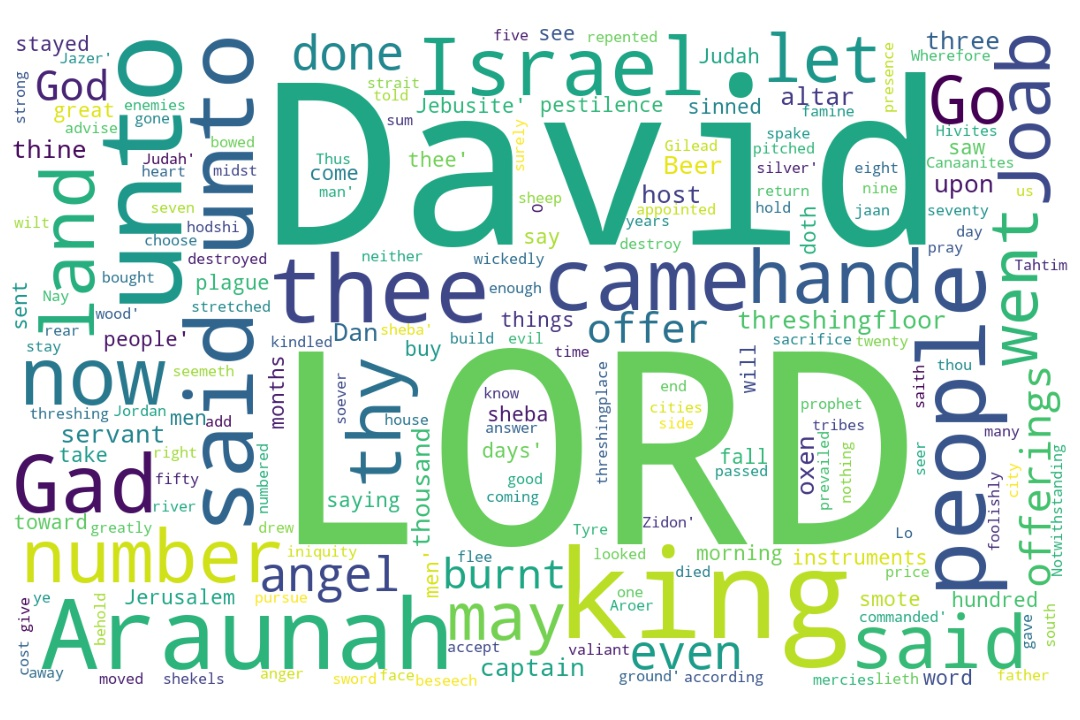
\includegraphics[width=\linewidth]{10OT-2Samuel/2Samuel24-WordCloud.jpg}
  \caption{1 Samuel 24 Word Cloud}
  \label{fig:1 Samuel 24 Word Cloud}
\end{figure}

%%%%%%%%%%%%%%%%%%%%%%%%%%%%%%%%%%%%%%%%%
%%%%%%%%%%%%%%%%%%%%%%%%%%%%%%%%%%%%%%%%%


\marginpar{\scriptsize \centering \fcolorbox{bone}{lime}{\textbf{CENSUS AND SACRIFICE}}\\ (2 Samuel 24:1--25) 
\begin{compactenum}[I.][8]
    \item A  \textbf{Census} \index[scripture]{2Samuel!2Sa 24:02}(2Sa 24:2)
    \item The  \textbf{Suggestion} \index[scripture]{2Samuel!2Sa 24:03}(2Sa 24:3) 
    \item The \textbf{Sum} \index[scripture]{2Samuel!2Sa 24:09} (2Sa 24:9)
    \item \textbf{Second} Thoughts \index[scripture]{2Samuel!2Sa 24:10} (2Sa 24:10)
    \item The \textbf{Sickness} \index[scripture]{2Samuel!2Sa 24:15} (2Sa 24:15)
    \item A \textbf{Sermon} \index[scripture]{2Samuel!2Sa 24:18} (2Sa 24:18) 
    \item The \textbf{Sacrifice} \index[scripture]{2Samuel!2Sa 24:25}(2Sa 24:25)
\end{compactenum} }

\footnote{\textcolor[cmyk]{0.99998,1,0,0}{\hyperlink{TOC}{Return to end of Table of Contents.}}}\footnote{\href{https://audiobible.com/bible/2_samuel_24.html}{\textcolor[cmyk]{0.99998,1,0,0}{2 Samuel 24 Audio}}}\textcolor[cmyk]{0.99998,1,0,0}{And again the anger of the LORD was kindled against Israel, and he moved  \fcolorbox{bone}{bone}{David} against them to say, \fcolorbox{bone}{lime}{Go, number Israel} and Judah.}
[2] \textcolor[cmyk]{0.99998,1,0,0}{For  \fcolorbox{bone}{bone}{the king}  \fcolorbox{bone}{bone}{said} to Joab the captain of the host, which \emph{was} with him, Go now through all the tribes of Israel, from Dan even to Beer-sheba, and number ye the people, that I may know the number of the people.}
[3] \textcolor[cmyk]{0.99998,1,0,0}{And Joab  \fcolorbox{bone}{bone}{said} unto  \fcolorbox{bone}{bone}{the king}, Now the LORD thy God add unto the people, how many soever they be, an hundredfold, and that the eyes of my lord  \fcolorbox{bone}{bone}{the king} may see \emph{it}: \fcolorbox{bone}{lime}{but why} doth my lord  \fcolorbox{bone}{bone}{the king} delight in this thing?}
[4] \textcolor[cmyk]{0.99998,1,0,0}{Notwithstanding the king's word prevailed against Joab, and against the captains of the host. And Joab and the captains of the host went out from the presence of  \fcolorbox{bone}{bone}{the king}, to number the people of Israel.}
[5] \textcolor[cmyk]{0.99998,1,0,0}{And they passed over Jordan, and pitched in Aroer, on the right side of the city that \emph{lieth} in the midst of the river of Gad, and toward Jazer:}\\
\\
\P \textcolor[cmyk]{0.99998,1,0,0}{Then they came to Gilead, and to the land of Tahtim-hodshi; and they came to Dan-jaan, and about to Zidon,}
[7] \textcolor[cmyk]{0.99998,1,0,0}{And came to the strong hold of Tyre, and to all the cities of the Hivites, and of the Canaanites: and they went out to the south of Judah, \emph{even} to Beer-sheba.}
[8] \textcolor[cmyk]{0.99998,1,0,0}{So when they had gone through all the land, they came to Jerusalem at the end of nine months and twenty days.}
[9] \textcolor[cmyk]{0.99998,1,0,0}{And Joab gave up \fcolorbox{bone}{lime}{the sum} of the number of the people unto  \fcolorbox{bone}{bone}{the king}: and there were in Israel eight hundred thousand valiant men that drew the sword; and the men of Judah \emph{were} five hundred thousand men.}\marginpar{\scriptsize \textcolor[rgb]{0.00,0.545,0.269}{$\rightarrow$800,000 + 500,000 = 1,300,000. }}\\
\\
\P \textcolor[cmyk]{0.99998,1,0,0}{And David's \fcolorbox{bone}{lime}{heart smote him} after that he had numbered the people. And  \fcolorbox{bone}{bone}{David}  \fcolorbox{bone}{bone}{said} unto the LORD, I have sinned greatly in that I have done: and now, I beseech thee, O LORD, take away the iniquity of thy servant; for I have done very foolishly.}
[11] \textcolor[cmyk]{0.99998,1,0,0}{For when David was up in the morning, the word of the LORD came unto the prophet Gad, David's seer, saying,}
[12] \textcolor[cmyk]{0.99998,1,0,0}{Go and say unto  \fcolorbox{bone}{bone}{David}, Thus saith the LORD, I offer thee three \emph{things}; choose thee one of them, that I may \emph{do} \emph{it} unto thee.}
[13] \textcolor[cmyk]{0.99998,1,0,0}{So Gad came to  \fcolorbox{bone}{bone}{David}, and told him, and  \fcolorbox{bone}{bone}{said} unto him, Shall seven years of famine come unto thee in thy land? or wilt thou flee three months before thine enemies, while they pursue thee? or that there be three days' pestilence in thy land? now advise, and see what answer I shall return to him that sent me.}
[14] \textcolor[cmyk]{0.99998,1,0,0}{And  \fcolorbox{bone}{bone}{David}  \fcolorbox{bone}{bone}{said} unto Gad, I am in a great strait: let us fall now into the hand of the LORD; for his mercies \emph{are} great: and let me not fall into the hand of man.}\\
\\
\P \textcolor[cmyk]{0.99998,1,0,0}{So the LORD sent a \fcolorbox{bone}{lime}{pestilence} upon Israel from the morning even to the time appointed: and there died of the people from Dan even to Beer-sheba seventy thousand men.}
[16] \textcolor[cmyk]{0.99998,1,0,0}{And when the angel stretched out his hand upon Jerusalem to destroy it, the LORD repented him of the evil, and  \fcolorbox{bone}{bone}{said} to the angel that destroyed the people, It is enough: stay now thine hand. And the angel of the LORD was by the threshingplace of Araunah the Jebusite.}
[17] \textcolor[cmyk]{0.99998,1,0,0}{And  \fcolorbox{bone}{bone}{David} spake unto the LORD when he saw the angel that smote the people, and  \fcolorbox{bone}{bone}{said}, Lo, I have sinned, and I have done wickedly: but these sheep, what have they done? let thine hand, I pray thee, be against me, and against my father's house.}\\
\\
\P \textcolor[cmyk]{0.99998,1,0,0}{And \fcolorbox{bone}{lime}{Gad came that day} to  \fcolorbox{bone}{bone}{David}, and  \fcolorbox{bone}{bone}{said} unto him, Go up, rear an altar unto the LORD in the threshingfloor of Araunah the Jebusite.}
[19] \textcolor[cmyk]{0.99998,1,0,0}{And  \fcolorbox{bone}{bone}{David}, according to the saying of Gad, went up as the LORD commanded.}
[20] \textcolor[cmyk]{0.99998,1,0,0}{And Araunah looked, and saw  \fcolorbox{bone}{bone}{the king} and his servants coming on toward him: and Araunah went out, and bowed himself before  \fcolorbox{bone}{bone}{the king} on his face upon the ground.}
[21] \textcolor[cmyk]{0.99998,1,0,0}{And Araunah  \fcolorbox{bone}{bone}{said}, Wherefore is my lord  \fcolorbox{bone}{bone}{the king} come to his servant? And  \fcolorbox{bone}{bone}{David}  \fcolorbox{bone}{bone}{said}, To buy the threshingfloor of thee, to build an altar unto the LORD, that the plague may be stayed from the people.}
[22] \textcolor[cmyk]{0.99998,1,0,0}{And Araunah  \fcolorbox{bone}{bone}{said} unto  \fcolorbox{bone}{bone}{David}, Let my lord  \fcolorbox{bone}{bone}{the king} take and offer up what \emph{seemeth} good unto him: behold, \emph{here} \emph{be} oxen for burnt sacrifice, and threshing instruments and \emph{other} instruments of the oxen for wood.}
[23] \textcolor[cmyk]{0.99998,1,0,0}{All these \emph{things} did Araunah, \emph{as} a king, give unto  \fcolorbox{bone}{bone}{the king}. And Araunah  \fcolorbox{bone}{bone}{said} unto  \fcolorbox{bone}{bone}{the king}, The LORD thy God accept thee.}
[24] \textcolor[cmyk]{0.99998,1,0,0}{And  \fcolorbox{bone}{bone}{the king}  \fcolorbox{bone}{bone}{said} unto Araunah, Nay; but I will surely buy \emph{it} of thee at a price: neither will I offer burnt offerings unto the LORD my God of that which doth cost me nothing. So  \fcolorbox{bone}{bone}{David} bought the threshingfloor and the oxen for fifty shekels of silver.}
[25] \textcolor[cmyk]{0.99998,1,0,0}{And  \fcolorbox{bone}{bone}{David} built there an altar unto the LORD, and offered burnt offerings and \fcolorbox{bone}{lime}{peace offerings}. So the LORD was intreated for the land, and the plague was stayed from Israel.}
\index[NWIV]{24!2Samuel!2Sa 24:1}\index[AWIP]{And!2Samuel!2Sa 24:1}\index[AWIP]{again!2Samuel!2Sa 24:1}\index[AWIP]{the!2Samuel!2Sa 24:1}\index[AWIP]{the!2Samuel!2Sa 24:1 (2)}\index[AWIP]{anger!2Samuel!2Sa 24:1}\index[AWIP]{of!2Samuel!2Sa 24:1}\index[AWIP]{LORD!2Samuel!2Sa 24:1}\index[AWIP]{was!2Samuel!2Sa 24:1}\index[AWIP]{kindled!2Samuel!2Sa 24:1}\index[AWIP]{against!2Samuel!2Sa 24:1}\index[AWIP]{against!2Samuel!2Sa 24:1 (2)}\index[AWIP]{Israel!2Samuel!2Sa 24:1}\index[AWIP]{Israel!2Samuel!2Sa 24:1 (2)}\index[AWIP]{and!2Samuel!2Sa 24:1}\index[AWIP]{and!2Samuel!2Sa 24:1 (2)}\index[AWIP]{he!2Samuel!2Sa 24:1}\index[AWIP]{moved!2Samuel!2Sa 24:1}\index[AWIP]{David!2Samuel!2Sa 24:1}\index[AWIP]{them!2Samuel!2Sa 24:1}\index[AWIP]{to!2Samuel!2Sa 24:1}\index[AWIP]{say!2Samuel!2Sa 24:1}\index[AWIP]{Go!2Samuel!2Sa 24:1}\index[AWIP]{number!2Samuel!2Sa 24:1}\index[AWIP]{Judah!2Samuel!2Sa 24:1}

\index[NWIV]{42!2Samuel!2Sa 24:2}\index[AWIP]{For!2Samuel!2Sa 24:2}\index[AWIP]{the!2Samuel!2Sa 24:2}\index[AWIP]{the!2Samuel!2Sa 24:2 (2)}\index[AWIP]{the!2Samuel!2Sa 24:2 (3)}\index[AWIP]{the!2Samuel!2Sa 24:2 (4)}\index[AWIP]{the!2Samuel!2Sa 24:2 (5)}\index[AWIP]{the!2Samuel!2Sa 24:2 (6)}\index[AWIP]{the!2Samuel!2Sa 24:2 (7)}\index[AWIP]{king!2Samuel!2Sa 24:2}\index[AWIP]{said!2Samuel!2Sa 24:2}\index[AWIP]{to!2Samuel!2Sa 24:2}\index[AWIP]{to!2Samuel!2Sa 24:2 (2)}\index[AWIP]{Joab!2Samuel!2Sa 24:2}\index[AWIP]{captain!2Samuel!2Sa 24:2}\index[AWIP]{of!2Samuel!2Sa 24:2}\index[AWIP]{of!2Samuel!2Sa 24:2 (2)}\index[AWIP]{of!2Samuel!2Sa 24:2 (3)}\index[AWIP]{host!2Samuel!2Sa 24:2}\index[AWIP]{which!2Samuel!2Sa 24:2}\index[AWIP]{\emph{was}!2Samuel!2Sa 24:2}\index[AWIP]{with!2Samuel!2Sa 24:2}\index[AWIP]{him!2Samuel!2Sa 24:2}\index[AWIP]{Go!2Samuel!2Sa 24:2}\index[AWIP]{now!2Samuel!2Sa 24:2}\index[AWIP]{through!2Samuel!2Sa 24:2}\index[AWIP]{all!2Samuel!2Sa 24:2}\index[AWIP]{tribes!2Samuel!2Sa 24:2}\index[AWIP]{Israel!2Samuel!2Sa 24:2}\index[AWIP]{from!2Samuel!2Sa 24:2}\index[AWIP]{Dan!2Samuel!2Sa 24:2}\index[AWIP]{even!2Samuel!2Sa 24:2}\index[AWIP]{Beer-sheba!2Samuel!2Sa 24:2}\index[AWIP]{and!2Samuel!2Sa 24:2}\index[AWIP]{number!2Samuel!2Sa 24:2}\index[AWIP]{number!2Samuel!2Sa 24:2 (2)}\index[AWIP]{ye!2Samuel!2Sa 24:2}\index[AWIP]{people!2Samuel!2Sa 24:2}\index[AWIP]{people!2Samuel!2Sa 24:2 (2)}\index[AWIP]{that!2Samuel!2Sa 24:2}\index[AWIP]{I!2Samuel!2Sa 24:2}\index[AWIP]{may!2Samuel!2Sa 24:2}\index[AWIP]{know!2Samuel!2Sa 24:2}\index[AWIP]{\emph{was}!2Samuel!2Sa 24:2}

\index[NWIV]{45!2Samuel!2Sa 24:3}\index[AWIP]{And!2Samuel!2Sa 24:3}\index[AWIP]{Joab!2Samuel!2Sa 24:3}\index[AWIP]{said!2Samuel!2Sa 24:3}\index[AWIP]{unto!2Samuel!2Sa 24:3}\index[AWIP]{unto!2Samuel!2Sa 24:3 (2)}\index[AWIP]{the!2Samuel!2Sa 24:3}\index[AWIP]{the!2Samuel!2Sa 24:3 (2)}\index[AWIP]{the!2Samuel!2Sa 24:3 (3)}\index[AWIP]{the!2Samuel!2Sa 24:3 (4)}\index[AWIP]{the!2Samuel!2Sa 24:3 (5)}\index[AWIP]{the!2Samuel!2Sa 24:3 (6)}\index[AWIP]{king!2Samuel!2Sa 24:3}\index[AWIP]{king!2Samuel!2Sa 24:3 (2)}\index[AWIP]{king!2Samuel!2Sa 24:3 (3)}\index[AWIP]{Now!2Samuel!2Sa 24:3}\index[AWIP]{LORD!2Samuel!2Sa 24:3}\index[AWIP]{thy!2Samuel!2Sa 24:3}\index[AWIP]{God!2Samuel!2Sa 24:3}\index[AWIP]{add!2Samuel!2Sa 24:3}\index[AWIP]{people!2Samuel!2Sa 24:3}\index[AWIP]{how!2Samuel!2Sa 24:3}\index[AWIP]{many!2Samuel!2Sa 24:3}\index[AWIP]{soever!2Samuel!2Sa 24:3}\index[AWIP]{they!2Samuel!2Sa 24:3}\index[AWIP]{be!2Samuel!2Sa 24:3}\index[AWIP]{an!2Samuel!2Sa 24:3}\index[AWIP]{hundredfold!2Samuel!2Sa 24:3}\index[AWIP]{and!2Samuel!2Sa 24:3}\index[AWIP]{that!2Samuel!2Sa 24:3}\index[AWIP]{eyes!2Samuel!2Sa 24:3}\index[AWIP]{of!2Samuel!2Sa 24:3}\index[AWIP]{my!2Samuel!2Sa 24:3}\index[AWIP]{my!2Samuel!2Sa 24:3 (2)}\index[AWIP]{lord!2Samuel!2Sa 24:3}\index[AWIP]{lord!2Samuel!2Sa 24:3 (2)}\index[AWIP]{may!2Samuel!2Sa 24:3}\index[AWIP]{see!2Samuel!2Sa 24:3}\index[AWIP]{\emph{it}!2Samuel!2Sa 24:3}\index[AWIP]{but!2Samuel!2Sa 24:3}\index[AWIP]{why!2Samuel!2Sa 24:3}\index[AWIP]{doth!2Samuel!2Sa 24:3}\index[AWIP]{delight!2Samuel!2Sa 24:3}\index[AWIP]{in!2Samuel!2Sa 24:3}\index[AWIP]{this!2Samuel!2Sa 24:3}\index[AWIP]{thing?!2Samuel!2Sa 24:3}\index[AWIP]{\emph{it}!2Samuel!2Sa 24:3}

\index[NWIV]{36!2Samuel!2Sa 24:4}\index[AWIP]{Notwithstanding!2Samuel!2Sa 24:4}\index[AWIP]{the!2Samuel!2Sa 24:4}\index[AWIP]{the!2Samuel!2Sa 24:4 (2)}\index[AWIP]{the!2Samuel!2Sa 24:4 (3)}\index[AWIP]{the!2Samuel!2Sa 24:4 (4)}\index[AWIP]{the!2Samuel!2Sa 24:4 (5)}\index[AWIP]{the!2Samuel!2Sa 24:4 (6)}\index[AWIP]{the!2Samuel!2Sa 24:4 (7)}\index[AWIP]{the!2Samuel!2Sa 24:4 (8)}\index[AWIP]{king's!2Samuel!2Sa 24:4}\index[AWIP]{word!2Samuel!2Sa 24:4}\index[AWIP]{prevailed!2Samuel!2Sa 24:4}\index[AWIP]{against!2Samuel!2Sa 24:4}\index[AWIP]{against!2Samuel!2Sa 24:4 (2)}\index[AWIP]{Joab!2Samuel!2Sa 24:4}\index[AWIP]{Joab!2Samuel!2Sa 24:4 (2)}\index[AWIP]{and!2Samuel!2Sa 24:4}\index[AWIP]{and!2Samuel!2Sa 24:4 (2)}\index[AWIP]{captains!2Samuel!2Sa 24:4}\index[AWIP]{captains!2Samuel!2Sa 24:4 (2)}\index[AWIP]{of!2Samuel!2Sa 24:4}\index[AWIP]{of!2Samuel!2Sa 24:4 (2)}\index[AWIP]{of!2Samuel!2Sa 24:4 (3)}\index[AWIP]{of!2Samuel!2Sa 24:4 (4)}\index[AWIP]{host!2Samuel!2Sa 24:4}\index[AWIP]{host!2Samuel!2Sa 24:4 (2)}\index[AWIP]{And!2Samuel!2Sa 24:4}\index[AWIP]{went!2Samuel!2Sa 24:4}\index[AWIP]{out!2Samuel!2Sa 24:4}\index[AWIP]{from!2Samuel!2Sa 24:4}\index[AWIP]{presence!2Samuel!2Sa 24:4}\index[AWIP]{king!2Samuel!2Sa 24:4}\index[AWIP]{to!2Samuel!2Sa 24:4}\index[AWIP]{number!2Samuel!2Sa 24:4}\index[AWIP]{people!2Samuel!2Sa 24:4}\index[AWIP]{Israel!2Samuel!2Sa 24:4}

\index[NWIV]{29!2Samuel!2Sa 24:5}\index[AWIP]{And!2Samuel!2Sa 24:5}\index[AWIP]{they!2Samuel!2Sa 24:5}\index[AWIP]{passed!2Samuel!2Sa 24:5}\index[AWIP]{over!2Samuel!2Sa 24:5}\index[AWIP]{Jordan!2Samuel!2Sa 24:5}\index[AWIP]{and!2Samuel!2Sa 24:5}\index[AWIP]{and!2Samuel!2Sa 24:5 (2)}\index[AWIP]{pitched!2Samuel!2Sa 24:5}\index[AWIP]{in!2Samuel!2Sa 24:5}\index[AWIP]{in!2Samuel!2Sa 24:5 (2)}\index[AWIP]{Aroer!2Samuel!2Sa 24:5}\index[AWIP]{on!2Samuel!2Sa 24:5}\index[AWIP]{the!2Samuel!2Sa 24:5}\index[AWIP]{the!2Samuel!2Sa 24:5 (2)}\index[AWIP]{the!2Samuel!2Sa 24:5 (3)}\index[AWIP]{the!2Samuel!2Sa 24:5 (4)}\index[AWIP]{right!2Samuel!2Sa 24:5}\index[AWIP]{side!2Samuel!2Sa 24:5}\index[AWIP]{of!2Samuel!2Sa 24:5}\index[AWIP]{of!2Samuel!2Sa 24:5 (2)}\index[AWIP]{of!2Samuel!2Sa 24:5 (3)}\index[AWIP]{city!2Samuel!2Sa 24:5}\index[AWIP]{that!2Samuel!2Sa 24:5}\index[AWIP]{\emph{lieth}!2Samuel!2Sa 24:5}\index[AWIP]{midst!2Samuel!2Sa 24:5}\index[AWIP]{river!2Samuel!2Sa 24:5}\index[AWIP]{Gad!2Samuel!2Sa 24:5}\index[AWIP]{toward!2Samuel!2Sa 24:5}\index[AWIP]{Jazer!2Samuel!2Sa 24:5}\index[AWIP]{\emph{lieth}!2Samuel!2Sa 24:5}

\index[NWIV]{20!2Samuel!2Sa 24:6}\index[AWIP]{Then!2Samuel!2Sa 24:6}\index[AWIP]{they!2Samuel!2Sa 24:6}\index[AWIP]{they!2Samuel!2Sa 24:6 (2)}\index[AWIP]{came!2Samuel!2Sa 24:6}\index[AWIP]{came!2Samuel!2Sa 24:6 (2)}\index[AWIP]{to!2Samuel!2Sa 24:6}\index[AWIP]{to!2Samuel!2Sa 24:6 (2)}\index[AWIP]{to!2Samuel!2Sa 24:6 (3)}\index[AWIP]{to!2Samuel!2Sa 24:6 (4)}\index[AWIP]{Gilead!2Samuel!2Sa 24:6}\index[AWIP]{and!2Samuel!2Sa 24:6}\index[AWIP]{and!2Samuel!2Sa 24:6 (2)}\index[AWIP]{and!2Samuel!2Sa 24:6 (3)}\index[AWIP]{the!2Samuel!2Sa 24:6}\index[AWIP]{land!2Samuel!2Sa 24:6}\index[AWIP]{of!2Samuel!2Sa 24:6}\index[AWIP]{Tahtim-hodshi!2Samuel!2Sa 24:6}\index[AWIP]{Dan-jaan!2Samuel!2Sa 24:6}\index[AWIP]{about!2Samuel!2Sa 24:6}\index[AWIP]{Zidon!2Samuel!2Sa 24:6}

\index[NWIV]{32!2Samuel!2Sa 24:7}\index[AWIP]{And!2Samuel!2Sa 24:7}\index[AWIP]{came!2Samuel!2Sa 24:7}\index[AWIP]{to!2Samuel!2Sa 24:7}\index[AWIP]{to!2Samuel!2Sa 24:7 (2)}\index[AWIP]{to!2Samuel!2Sa 24:7 (3)}\index[AWIP]{to!2Samuel!2Sa 24:7 (4)}\index[AWIP]{the!2Samuel!2Sa 24:7}\index[AWIP]{the!2Samuel!2Sa 24:7 (2)}\index[AWIP]{the!2Samuel!2Sa 24:7 (3)}\index[AWIP]{the!2Samuel!2Sa 24:7 (4)}\index[AWIP]{the!2Samuel!2Sa 24:7 (5)}\index[AWIP]{strong!2Samuel!2Sa 24:7}\index[AWIP]{hold!2Samuel!2Sa 24:7}\index[AWIP]{of!2Samuel!2Sa 24:7}\index[AWIP]{of!2Samuel!2Sa 24:7 (2)}\index[AWIP]{of!2Samuel!2Sa 24:7 (3)}\index[AWIP]{of!2Samuel!2Sa 24:7 (4)}\index[AWIP]{Tyre!2Samuel!2Sa 24:7}\index[AWIP]{and!2Samuel!2Sa 24:7}\index[AWIP]{and!2Samuel!2Sa 24:7 (2)}\index[AWIP]{and!2Samuel!2Sa 24:7 (3)}\index[AWIP]{all!2Samuel!2Sa 24:7}\index[AWIP]{cities!2Samuel!2Sa 24:7}\index[AWIP]{Hivites!2Samuel!2Sa 24:7}\index[AWIP]{Canaanites!2Samuel!2Sa 24:7}\index[AWIP]{they!2Samuel!2Sa 24:7}\index[AWIP]{went!2Samuel!2Sa 24:7}\index[AWIP]{out!2Samuel!2Sa 24:7}\index[AWIP]{south!2Samuel!2Sa 24:7}\index[AWIP]{Judah!2Samuel!2Sa 24:7}\index[AWIP]{\emph{even}!2Samuel!2Sa 24:7}\index[AWIP]{Beer-sheba!2Samuel!2Sa 24:7}\index[AWIP]{\emph{even}!2Samuel!2Sa 24:7}

\index[NWIV]{22!2Samuel!2Sa 24:8}\index[AWIP]{So!2Samuel!2Sa 24:8}\index[AWIP]{when!2Samuel!2Sa 24:8}\index[AWIP]{they!2Samuel!2Sa 24:8}\index[AWIP]{they!2Samuel!2Sa 24:8 (2)}\index[AWIP]{had!2Samuel!2Sa 24:8}\index[AWIP]{gone!2Samuel!2Sa 24:8}\index[AWIP]{through!2Samuel!2Sa 24:8}\index[AWIP]{all!2Samuel!2Sa 24:8}\index[AWIP]{the!2Samuel!2Sa 24:8}\index[AWIP]{the!2Samuel!2Sa 24:8 (2)}\index[AWIP]{land!2Samuel!2Sa 24:8}\index[AWIP]{came!2Samuel!2Sa 24:8}\index[AWIP]{to!2Samuel!2Sa 24:8}\index[AWIP]{Jerusalem!2Samuel!2Sa 24:8}\index[AWIP]{at!2Samuel!2Sa 24:8}\index[AWIP]{end!2Samuel!2Sa 24:8}\index[AWIP]{of!2Samuel!2Sa 24:8}\index[AWIP]{nine!2Samuel!2Sa 24:8}\index[AWIP]{months!2Samuel!2Sa 24:8}\index[AWIP]{and!2Samuel!2Sa 24:8}\index[AWIP]{twenty!2Samuel!2Sa 24:8}\index[AWIP]{days!2Samuel!2Sa 24:8}

\index[NWIV]{39!2Samuel!2Sa 24:9}\index[AWIP]{And!2Samuel!2Sa 24:9}\index[AWIP]{Joab!2Samuel!2Sa 24:9}\index[AWIP]{gave!2Samuel!2Sa 24:9}\index[AWIP]{up!2Samuel!2Sa 24:9}\index[AWIP]{the!2Samuel!2Sa 24:9}\index[AWIP]{the!2Samuel!2Sa 24:9 (2)}\index[AWIP]{the!2Samuel!2Sa 24:9 (3)}\index[AWIP]{the!2Samuel!2Sa 24:9 (4)}\index[AWIP]{the!2Samuel!2Sa 24:9 (5)}\index[AWIP]{the!2Samuel!2Sa 24:9 (6)}\index[AWIP]{sum!2Samuel!2Sa 24:9}\index[AWIP]{of!2Samuel!2Sa 24:9}\index[AWIP]{of!2Samuel!2Sa 24:9 (2)}\index[AWIP]{of!2Samuel!2Sa 24:9 (3)}\index[AWIP]{number!2Samuel!2Sa 24:9}\index[AWIP]{people!2Samuel!2Sa 24:9}\index[AWIP]{unto!2Samuel!2Sa 24:9}\index[AWIP]{king!2Samuel!2Sa 24:9}\index[AWIP]{and!2Samuel!2Sa 24:9}\index[AWIP]{and!2Samuel!2Sa 24:9 (2)}\index[AWIP]{there!2Samuel!2Sa 24:9}\index[AWIP]{were!2Samuel!2Sa 24:9}\index[AWIP]{in!2Samuel!2Sa 24:9}\index[AWIP]{Israel!2Samuel!2Sa 24:9}\index[AWIP]{eight!2Samuel!2Sa 24:9}\index[AWIP]{hundred!2Samuel!2Sa 24:9}\index[AWIP]{hundred!2Samuel!2Sa 24:9 (2)}\index[AWIP]{thousand!2Samuel!2Sa 24:9}\index[AWIP]{thousand!2Samuel!2Sa 24:9 (2)}\index[AWIP]{valiant!2Samuel!2Sa 24:9}\index[AWIP]{men!2Samuel!2Sa 24:9}\index[AWIP]{men!2Samuel!2Sa 24:9 (2)}\index[AWIP]{men!2Samuel!2Sa 24:9 (3)}\index[AWIP]{that!2Samuel!2Sa 24:9}\index[AWIP]{drew!2Samuel!2Sa 24:9}\index[AWIP]{sword!2Samuel!2Sa 24:9}\index[AWIP]{Judah!2Samuel!2Sa 24:9}\index[AWIP]{\emph{were}!2Samuel!2Sa 24:9}\index[AWIP]{five!2Samuel!2Sa 24:9}\index[AWIP]{\emph{were}!2Samuel!2Sa 24:9}

\index[NWIV]{47!2Samuel!2Sa 24:10}\index[AWIP]{And!2Samuel!2Sa 24:10}\index[AWIP]{And!2Samuel!2Sa 24:10 (2)}\index[AWIP]{David's!2Samuel!2Sa 24:10}\index[AWIP]{heart!2Samuel!2Sa 24:10}\index[AWIP]{smote!2Samuel!2Sa 24:10}\index[AWIP]{him!2Samuel!2Sa 24:10}\index[AWIP]{after!2Samuel!2Sa 24:10}\index[AWIP]{that!2Samuel!2Sa 24:10}\index[AWIP]{that!2Samuel!2Sa 24:10 (2)}\index[AWIP]{he!2Samuel!2Sa 24:10}\index[AWIP]{had!2Samuel!2Sa 24:10}\index[AWIP]{numbered!2Samuel!2Sa 24:10}\index[AWIP]{the!2Samuel!2Sa 24:10}\index[AWIP]{the!2Samuel!2Sa 24:10 (2)}\index[AWIP]{the!2Samuel!2Sa 24:10 (3)}\index[AWIP]{people!2Samuel!2Sa 24:10}\index[AWIP]{David!2Samuel!2Sa 24:10}\index[AWIP]{said!2Samuel!2Sa 24:10}\index[AWIP]{unto!2Samuel!2Sa 24:10}\index[AWIP]{LORD!2Samuel!2Sa 24:10}\index[AWIP]{LORD!2Samuel!2Sa 24:10 (2)}\index[AWIP]{I!2Samuel!2Sa 24:10}\index[AWIP]{I!2Samuel!2Sa 24:10 (2)}\index[AWIP]{I!2Samuel!2Sa 24:10 (3)}\index[AWIP]{I!2Samuel!2Sa 24:10 (4)}\index[AWIP]{have!2Samuel!2Sa 24:10}\index[AWIP]{have!2Samuel!2Sa 24:10 (2)}\index[AWIP]{have!2Samuel!2Sa 24:10 (3)}\index[AWIP]{sinned!2Samuel!2Sa 24:10}\index[AWIP]{greatly!2Samuel!2Sa 24:10}\index[AWIP]{in!2Samuel!2Sa 24:10}\index[AWIP]{done!2Samuel!2Sa 24:10}\index[AWIP]{done!2Samuel!2Sa 24:10 (2)}\index[AWIP]{and!2Samuel!2Sa 24:10}\index[AWIP]{now!2Samuel!2Sa 24:10}\index[AWIP]{beseech!2Samuel!2Sa 24:10}\index[AWIP]{thee!2Samuel!2Sa 24:10}\index[AWIP]{O!2Samuel!2Sa 24:10}\index[AWIP]{take!2Samuel!2Sa 24:10}\index[AWIP]{away!2Samuel!2Sa 24:10}\index[AWIP]{iniquity!2Samuel!2Sa 24:10}\index[AWIP]{of!2Samuel!2Sa 24:10}\index[AWIP]{thy!2Samuel!2Sa 24:10}\index[AWIP]{servant!2Samuel!2Sa 24:10}\index[AWIP]{for!2Samuel!2Sa 24:10}\index[AWIP]{very!2Samuel!2Sa 24:10}\index[AWIP]{foolishly!2Samuel!2Sa 24:10}

\index[NWIV]{21!2Samuel!2Sa 24:11}\index[AWIP]{For!2Samuel!2Sa 24:11}\index[AWIP]{when!2Samuel!2Sa 24:11}\index[AWIP]{David!2Samuel!2Sa 24:11}\index[AWIP]{was!2Samuel!2Sa 24:11}\index[AWIP]{up!2Samuel!2Sa 24:11}\index[AWIP]{in!2Samuel!2Sa 24:11}\index[AWIP]{the!2Samuel!2Sa 24:11}\index[AWIP]{the!2Samuel!2Sa 24:11 (2)}\index[AWIP]{the!2Samuel!2Sa 24:11 (3)}\index[AWIP]{the!2Samuel!2Sa 24:11 (4)}\index[AWIP]{morning!2Samuel!2Sa 24:11}\index[AWIP]{word!2Samuel!2Sa 24:11}\index[AWIP]{of!2Samuel!2Sa 24:11}\index[AWIP]{LORD!2Samuel!2Sa 24:11}\index[AWIP]{came!2Samuel!2Sa 24:11}\index[AWIP]{unto!2Samuel!2Sa 24:11}\index[AWIP]{prophet!2Samuel!2Sa 24:11}\index[AWIP]{Gad!2Samuel!2Sa 24:11}\index[AWIP]{David's!2Samuel!2Sa 24:11}\index[AWIP]{seer!2Samuel!2Sa 24:11}\index[AWIP]{saying!2Samuel!2Sa 24:11}

\index[NWIV]{26!2Samuel!2Sa 24:12}\index[AWIP]{Go!2Samuel!2Sa 24:12}\index[AWIP]{and!2Samuel!2Sa 24:12}\index[AWIP]{say!2Samuel!2Sa 24:12}\index[AWIP]{unto!2Samuel!2Sa 24:12}\index[AWIP]{unto!2Samuel!2Sa 24:12 (2)}\index[AWIP]{David!2Samuel!2Sa 24:12}\index[AWIP]{Thus!2Samuel!2Sa 24:12}\index[AWIP]{saith!2Samuel!2Sa 24:12}\index[AWIP]{the!2Samuel!2Sa 24:12}\index[AWIP]{LORD!2Samuel!2Sa 24:12}\index[AWIP]{I!2Samuel!2Sa 24:12}\index[AWIP]{I!2Samuel!2Sa 24:12 (2)}\index[AWIP]{offer!2Samuel!2Sa 24:12}\index[AWIP]{thee!2Samuel!2Sa 24:12}\index[AWIP]{thee!2Samuel!2Sa 24:12 (2)}\index[AWIP]{thee!2Samuel!2Sa 24:12 (3)}\index[AWIP]{three!2Samuel!2Sa 24:12}\index[AWIP]{\emph{things}!2Samuel!2Sa 24:12}\index[AWIP]{choose!2Samuel!2Sa 24:12}\index[AWIP]{one!2Samuel!2Sa 24:12}\index[AWIP]{of!2Samuel!2Sa 24:12}\index[AWIP]{them!2Samuel!2Sa 24:12}\index[AWIP]{that!2Samuel!2Sa 24:12}\index[AWIP]{may!2Samuel!2Sa 24:12}\index[AWIP]{\emph{do}!2Samuel!2Sa 24:12}\index[AWIP]{\emph{it}!2Samuel!2Sa 24:12}\index[AWIP]{\emph{things}!2Samuel!2Sa 24:12}\index[AWIP]{\emph{do}!2Samuel!2Sa 24:12}\index[AWIP]{\emph{it}!2Samuel!2Sa 24:12}

\index[NWIV]{60!2Samuel!2Sa 24:13}\index[AWIP]{So!2Samuel!2Sa 24:13}\index[AWIP]{Gad!2Samuel!2Sa 24:13}\index[AWIP]{came!2Samuel!2Sa 24:13}\index[AWIP]{to!2Samuel!2Sa 24:13}\index[AWIP]{to!2Samuel!2Sa 24:13 (2)}\index[AWIP]{David!2Samuel!2Sa 24:13}\index[AWIP]{and!2Samuel!2Sa 24:13}\index[AWIP]{and!2Samuel!2Sa 24:13 (2)}\index[AWIP]{and!2Samuel!2Sa 24:13 (3)}\index[AWIP]{told!2Samuel!2Sa 24:13}\index[AWIP]{him!2Samuel!2Sa 24:13}\index[AWIP]{him!2Samuel!2Sa 24:13 (2)}\index[AWIP]{him!2Samuel!2Sa 24:13 (3)}\index[AWIP]{said!2Samuel!2Sa 24:13}\index[AWIP]{unto!2Samuel!2Sa 24:13}\index[AWIP]{unto!2Samuel!2Sa 24:13 (2)}\index[AWIP]{Shall!2Samuel!2Sa 24:13}\index[AWIP]{seven!2Samuel!2Sa 24:13}\index[AWIP]{years!2Samuel!2Sa 24:13}\index[AWIP]{of!2Samuel!2Sa 24:13}\index[AWIP]{famine!2Samuel!2Sa 24:13}\index[AWIP]{come!2Samuel!2Sa 24:13}\index[AWIP]{thee!2Samuel!2Sa 24:13}\index[AWIP]{in!2Samuel!2Sa 24:13}\index[AWIP]{in!2Samuel!2Sa 24:13 (2)}\index[AWIP]{thy!2Samuel!2Sa 24:13}\index[AWIP]{thy!2Samuel!2Sa 24:13 (2)}\index[AWIP]{land?!2Samuel!2Sa 24:13}\index[AWIP]{land?!2Samuel!2Sa 24:13 (2)}\index[AWIP]{or!2Samuel!2Sa 24:13}\index[AWIP]{or!2Samuel!2Sa 24:13 (2)}\index[AWIP]{wilt!2Samuel!2Sa 24:13}\index[AWIP]{thou!2Samuel!2Sa 24:13}\index[AWIP]{flee!2Samuel!2Sa 24:13}\index[AWIP]{three!2Samuel!2Sa 24:13}\index[AWIP]{three!2Samuel!2Sa 24:13 (2)}\index[AWIP]{months!2Samuel!2Sa 24:13}\index[AWIP]{before!2Samuel!2Sa 24:13}\index[AWIP]{thine!2Samuel!2Sa 24:13}\index[AWIP]{enemies!2Samuel!2Sa 24:13}\index[AWIP]{while!2Samuel!2Sa 24:13}\index[AWIP]{they!2Samuel!2Sa 24:13}\index[AWIP]{pursue!2Samuel!2Sa 24:13}\index[AWIP]{thee?!2Samuel!2Sa 24:13}\index[AWIP]{that!2Samuel!2Sa 24:13}\index[AWIP]{that!2Samuel!2Sa 24:13 (2)}\index[AWIP]{there!2Samuel!2Sa 24:13}\index[AWIP]{be!2Samuel!2Sa 24:13}\index[AWIP]{days'!2Samuel!2Sa 24:13}\index[AWIP]{pestilence!2Samuel!2Sa 24:13}\index[AWIP]{now!2Samuel!2Sa 24:13}\index[AWIP]{advise!2Samuel!2Sa 24:13}\index[AWIP]{see!2Samuel!2Sa 24:13}\index[AWIP]{what!2Samuel!2Sa 24:13}\index[AWIP]{answer!2Samuel!2Sa 24:13}\index[AWIP]{I!2Samuel!2Sa 24:13}\index[AWIP]{shall!2Samuel!2Sa 24:13}\index[AWIP]{return!2Samuel!2Sa 24:13}\index[AWIP]{sent!2Samuel!2Sa 24:13}\index[AWIP]{me!2Samuel!2Sa 24:13}

\index[NWIV]{36!2Samuel!2Sa 24:14}\index[AWIP]{And!2Samuel!2Sa 24:14}\index[AWIP]{David!2Samuel!2Sa 24:14}\index[AWIP]{said!2Samuel!2Sa 24:14}\index[AWIP]{unto!2Samuel!2Sa 24:14}\index[AWIP]{Gad!2Samuel!2Sa 24:14}\index[AWIP]{I!2Samuel!2Sa 24:14}\index[AWIP]{am!2Samuel!2Sa 24:14}\index[AWIP]{in!2Samuel!2Sa 24:14}\index[AWIP]{a!2Samuel!2Sa 24:14}\index[AWIP]{great!2Samuel!2Sa 24:14}\index[AWIP]{great!2Samuel!2Sa 24:14 (2)}\index[AWIP]{strait!2Samuel!2Sa 24:14}\index[AWIP]{let!2Samuel!2Sa 24:14}\index[AWIP]{let!2Samuel!2Sa 24:14 (2)}\index[AWIP]{us!2Samuel!2Sa 24:14}\index[AWIP]{fall!2Samuel!2Sa 24:14}\index[AWIP]{fall!2Samuel!2Sa 24:14 (2)}\index[AWIP]{now!2Samuel!2Sa 24:14}\index[AWIP]{into!2Samuel!2Sa 24:14}\index[AWIP]{into!2Samuel!2Sa 24:14 (2)}\index[AWIP]{the!2Samuel!2Sa 24:14}\index[AWIP]{the!2Samuel!2Sa 24:14 (2)}\index[AWIP]{the!2Samuel!2Sa 24:14 (3)}\index[AWIP]{hand!2Samuel!2Sa 24:14}\index[AWIP]{hand!2Samuel!2Sa 24:14 (2)}\index[AWIP]{of!2Samuel!2Sa 24:14}\index[AWIP]{of!2Samuel!2Sa 24:14 (2)}\index[AWIP]{LORD!2Samuel!2Sa 24:14}\index[AWIP]{for!2Samuel!2Sa 24:14}\index[AWIP]{his!2Samuel!2Sa 24:14}\index[AWIP]{mercies!2Samuel!2Sa 24:14}\index[AWIP]{\emph{are}!2Samuel!2Sa 24:14}\index[AWIP]{and!2Samuel!2Sa 24:14}\index[AWIP]{me!2Samuel!2Sa 24:14}\index[AWIP]{not!2Samuel!2Sa 24:14}\index[AWIP]{man!2Samuel!2Sa 24:14}\index[AWIP]{\emph{are}!2Samuel!2Sa 24:14}

\index[NWIV]{30!2Samuel!2Sa 24:15}\index[AWIP]{So!2Samuel!2Sa 24:15}\index[AWIP]{the!2Samuel!2Sa 24:15}\index[AWIP]{the!2Samuel!2Sa 24:15 (2)}\index[AWIP]{the!2Samuel!2Sa 24:15 (3)}\index[AWIP]{the!2Samuel!2Sa 24:15 (4)}\index[AWIP]{LORD!2Samuel!2Sa 24:15}\index[AWIP]{sent!2Samuel!2Sa 24:15}\index[AWIP]{a!2Samuel!2Sa 24:15}\index[AWIP]{pestilence!2Samuel!2Sa 24:15}\index[AWIP]{upon!2Samuel!2Sa 24:15}\index[AWIP]{Israel!2Samuel!2Sa 24:15}\index[AWIP]{from!2Samuel!2Sa 24:15}\index[AWIP]{from!2Samuel!2Sa 24:15 (2)}\index[AWIP]{morning!2Samuel!2Sa 24:15}\index[AWIP]{even!2Samuel!2Sa 24:15}\index[AWIP]{even!2Samuel!2Sa 24:15 (2)}\index[AWIP]{to!2Samuel!2Sa 24:15}\index[AWIP]{to!2Samuel!2Sa 24:15 (2)}\index[AWIP]{time!2Samuel!2Sa 24:15}\index[AWIP]{appointed!2Samuel!2Sa 24:15}\index[AWIP]{and!2Samuel!2Sa 24:15}\index[AWIP]{there!2Samuel!2Sa 24:15}\index[AWIP]{died!2Samuel!2Sa 24:15}\index[AWIP]{of!2Samuel!2Sa 24:15}\index[AWIP]{people!2Samuel!2Sa 24:15}\index[AWIP]{Dan!2Samuel!2Sa 24:15}\index[AWIP]{Beer-sheba!2Samuel!2Sa 24:15}\index[AWIP]{seventy!2Samuel!2Sa 24:15}\index[AWIP]{thousand!2Samuel!2Sa 24:15}\index[AWIP]{men!2Samuel!2Sa 24:15}

\index[NWIV]{50!2Samuel!2Sa 24:16}\index[AWIP]{And!2Samuel!2Sa 24:16}\index[AWIP]{And!2Samuel!2Sa 24:16 (2)}\index[AWIP]{when!2Samuel!2Sa 24:16}\index[AWIP]{the!2Samuel!2Sa 24:16}\index[AWIP]{the!2Samuel!2Sa 24:16 (2)}\index[AWIP]{the!2Samuel!2Sa 24:16 (3)}\index[AWIP]{the!2Samuel!2Sa 24:16 (4)}\index[AWIP]{the!2Samuel!2Sa 24:16 (5)}\index[AWIP]{the!2Samuel!2Sa 24:16 (6)}\index[AWIP]{the!2Samuel!2Sa 24:16 (7)}\index[AWIP]{the!2Samuel!2Sa 24:16 (8)}\index[AWIP]{the!2Samuel!2Sa 24:16 (9)}\index[AWIP]{angel!2Samuel!2Sa 24:16}\index[AWIP]{angel!2Samuel!2Sa 24:16 (2)}\index[AWIP]{angel!2Samuel!2Sa 24:16 (3)}\index[AWIP]{stretched!2Samuel!2Sa 24:16}\index[AWIP]{out!2Samuel!2Sa 24:16}\index[AWIP]{his!2Samuel!2Sa 24:16}\index[AWIP]{hand!2Samuel!2Sa 24:16}\index[AWIP]{hand!2Samuel!2Sa 24:16 (2)}\index[AWIP]{upon!2Samuel!2Sa 24:16}\index[AWIP]{Jerusalem!2Samuel!2Sa 24:16}\index[AWIP]{to!2Samuel!2Sa 24:16}\index[AWIP]{to!2Samuel!2Sa 24:16 (2)}\index[AWIP]{destroy!2Samuel!2Sa 24:16}\index[AWIP]{it!2Samuel!2Sa 24:16}\index[AWIP]{LORD!2Samuel!2Sa 24:16}\index[AWIP]{LORD!2Samuel!2Sa 24:16 (2)}\index[AWIP]{repented!2Samuel!2Sa 24:16}\index[AWIP]{him!2Samuel!2Sa 24:16}\index[AWIP]{of!2Samuel!2Sa 24:16}\index[AWIP]{of!2Samuel!2Sa 24:16 (2)}\index[AWIP]{of!2Samuel!2Sa 24:16 (3)}\index[AWIP]{evil!2Samuel!2Sa 24:16}\index[AWIP]{and!2Samuel!2Sa 24:16}\index[AWIP]{said!2Samuel!2Sa 24:16}\index[AWIP]{that!2Samuel!2Sa 24:16}\index[AWIP]{destroyed!2Samuel!2Sa 24:16}\index[AWIP]{people!2Samuel!2Sa 24:16}\index[AWIP]{It!2Samuel!2Sa 24:16}\index[AWIP]{is!2Samuel!2Sa 24:16}\index[AWIP]{enough!2Samuel!2Sa 24:16}\index[AWIP]{stay!2Samuel!2Sa 24:16}\index[AWIP]{now!2Samuel!2Sa 24:16}\index[AWIP]{thine!2Samuel!2Sa 24:16}\index[AWIP]{was!2Samuel!2Sa 24:16}\index[AWIP]{by!2Samuel!2Sa 24:16}\index[AWIP]{threshingplace!2Samuel!2Sa 24:16}\index[AWIP]{Araunah!2Samuel!2Sa 24:16}\index[AWIP]{Jebusite!2Samuel!2Sa 24:16}

\index[NWIV]{47!2Samuel!2Sa 24:17}\index[AWIP]{And!2Samuel!2Sa 24:17}\index[AWIP]{David!2Samuel!2Sa 24:17}\index[AWIP]{spake!2Samuel!2Sa 24:17}\index[AWIP]{unto!2Samuel!2Sa 24:17}\index[AWIP]{the!2Samuel!2Sa 24:17}\index[AWIP]{the!2Samuel!2Sa 24:17 (2)}\index[AWIP]{the!2Samuel!2Sa 24:17 (3)}\index[AWIP]{LORD!2Samuel!2Sa 24:17}\index[AWIP]{when!2Samuel!2Sa 24:17}\index[AWIP]{he!2Samuel!2Sa 24:17}\index[AWIP]{saw!2Samuel!2Sa 24:17}\index[AWIP]{angel!2Samuel!2Sa 24:17}\index[AWIP]{that!2Samuel!2Sa 24:17}\index[AWIP]{smote!2Samuel!2Sa 24:17}\index[AWIP]{people!2Samuel!2Sa 24:17}\index[AWIP]{and!2Samuel!2Sa 24:17}\index[AWIP]{and!2Samuel!2Sa 24:17 (2)}\index[AWIP]{and!2Samuel!2Sa 24:17 (3)}\index[AWIP]{said!2Samuel!2Sa 24:17}\index[AWIP]{Lo!2Samuel!2Sa 24:17}\index[AWIP]{I!2Samuel!2Sa 24:17}\index[AWIP]{I!2Samuel!2Sa 24:17 (2)}\index[AWIP]{I!2Samuel!2Sa 24:17 (3)}\index[AWIP]{have!2Samuel!2Sa 24:17}\index[AWIP]{have!2Samuel!2Sa 24:17 (2)}\index[AWIP]{have!2Samuel!2Sa 24:17 (3)}\index[AWIP]{sinned!2Samuel!2Sa 24:17}\index[AWIP]{done!2Samuel!2Sa 24:17}\index[AWIP]{wickedly!2Samuel!2Sa 24:17}\index[AWIP]{but!2Samuel!2Sa 24:17}\index[AWIP]{these!2Samuel!2Sa 24:17}\index[AWIP]{sheep!2Samuel!2Sa 24:17}\index[AWIP]{what!2Samuel!2Sa 24:17}\index[AWIP]{they!2Samuel!2Sa 24:17}\index[AWIP]{done?!2Samuel!2Sa 24:17}\index[AWIP]{let!2Samuel!2Sa 24:17}\index[AWIP]{thine!2Samuel!2Sa 24:17}\index[AWIP]{hand!2Samuel!2Sa 24:17}\index[AWIP]{pray!2Samuel!2Sa 24:17}\index[AWIP]{thee!2Samuel!2Sa 24:17}\index[AWIP]{be!2Samuel!2Sa 24:17}\index[AWIP]{against!2Samuel!2Sa 24:17}\index[AWIP]{against!2Samuel!2Sa 24:17 (2)}\index[AWIP]{me!2Samuel!2Sa 24:17}\index[AWIP]{my!2Samuel!2Sa 24:17}\index[AWIP]{father's!2Samuel!2Sa 24:17}\index[AWIP]{house!2Samuel!2Sa 24:17}

\index[NWIV]{26!2Samuel!2Sa 24:18}\index[AWIP]{And!2Samuel!2Sa 24:18}\index[AWIP]{Gad!2Samuel!2Sa 24:18}\index[AWIP]{came!2Samuel!2Sa 24:18}\index[AWIP]{that!2Samuel!2Sa 24:18}\index[AWIP]{day!2Samuel!2Sa 24:18}\index[AWIP]{to!2Samuel!2Sa 24:18}\index[AWIP]{David!2Samuel!2Sa 24:18}\index[AWIP]{and!2Samuel!2Sa 24:18}\index[AWIP]{said!2Samuel!2Sa 24:18}\index[AWIP]{unto!2Samuel!2Sa 24:18}\index[AWIP]{unto!2Samuel!2Sa 24:18 (2)}\index[AWIP]{him!2Samuel!2Sa 24:18}\index[AWIP]{Go!2Samuel!2Sa 24:18}\index[AWIP]{up!2Samuel!2Sa 24:18}\index[AWIP]{rear!2Samuel!2Sa 24:18}\index[AWIP]{an!2Samuel!2Sa 24:18}\index[AWIP]{altar!2Samuel!2Sa 24:18}\index[AWIP]{the!2Samuel!2Sa 24:18}\index[AWIP]{the!2Samuel!2Sa 24:18 (2)}\index[AWIP]{the!2Samuel!2Sa 24:18 (3)}\index[AWIP]{LORD!2Samuel!2Sa 24:18}\index[AWIP]{in!2Samuel!2Sa 24:18}\index[AWIP]{threshingfloor!2Samuel!2Sa 24:18}\index[AWIP]{of!2Samuel!2Sa 24:18}\index[AWIP]{Araunah!2Samuel!2Sa 24:18}\index[AWIP]{Jebusite!2Samuel!2Sa 24:18}

\index[NWIV]{14!2Samuel!2Sa 24:19}\index[AWIP]{And!2Samuel!2Sa 24:19}\index[AWIP]{David!2Samuel!2Sa 24:19}\index[AWIP]{according!2Samuel!2Sa 24:19}\index[AWIP]{to!2Samuel!2Sa 24:19}\index[AWIP]{the!2Samuel!2Sa 24:19}\index[AWIP]{the!2Samuel!2Sa 24:19 (2)}\index[AWIP]{saying!2Samuel!2Sa 24:19}\index[AWIP]{of!2Samuel!2Sa 24:19}\index[AWIP]{Gad!2Samuel!2Sa 24:19}\index[AWIP]{went!2Samuel!2Sa 24:19}\index[AWIP]{up!2Samuel!2Sa 24:19}\index[AWIP]{as!2Samuel!2Sa 24:19}\index[AWIP]{LORD!2Samuel!2Sa 24:19}\index[AWIP]{commanded!2Samuel!2Sa 24:19}

\index[NWIV]{30!2Samuel!2Sa 24:20}\index[AWIP]{And!2Samuel!2Sa 24:20}\index[AWIP]{Araunah!2Samuel!2Sa 24:20}\index[AWIP]{Araunah!2Samuel!2Sa 24:20 (2)}\index[AWIP]{looked!2Samuel!2Sa 24:20}\index[AWIP]{and!2Samuel!2Sa 24:20}\index[AWIP]{and!2Samuel!2Sa 24:20 (2)}\index[AWIP]{and!2Samuel!2Sa 24:20 (3)}\index[AWIP]{and!2Samuel!2Sa 24:20 (4)}\index[AWIP]{saw!2Samuel!2Sa 24:20}\index[AWIP]{the!2Samuel!2Sa 24:20}\index[AWIP]{the!2Samuel!2Sa 24:20 (2)}\index[AWIP]{the!2Samuel!2Sa 24:20 (3)}\index[AWIP]{king!2Samuel!2Sa 24:20}\index[AWIP]{king!2Samuel!2Sa 24:20 (2)}\index[AWIP]{his!2Samuel!2Sa 24:20}\index[AWIP]{his!2Samuel!2Sa 24:20 (2)}\index[AWIP]{servants!2Samuel!2Sa 24:20}\index[AWIP]{coming!2Samuel!2Sa 24:20}\index[AWIP]{on!2Samuel!2Sa 24:20}\index[AWIP]{on!2Samuel!2Sa 24:20 (2)}\index[AWIP]{toward!2Samuel!2Sa 24:20}\index[AWIP]{him!2Samuel!2Sa 24:20}\index[AWIP]{went!2Samuel!2Sa 24:20}\index[AWIP]{out!2Samuel!2Sa 24:20}\index[AWIP]{bowed!2Samuel!2Sa 24:20}\index[AWIP]{himself!2Samuel!2Sa 24:20}\index[AWIP]{before!2Samuel!2Sa 24:20}\index[AWIP]{face!2Samuel!2Sa 24:20}\index[AWIP]{upon!2Samuel!2Sa 24:20}\index[AWIP]{ground!2Samuel!2Sa 24:20}

\index[NWIV]{38!2Samuel!2Sa 24:21}\index[AWIP]{And!2Samuel!2Sa 24:21}\index[AWIP]{And!2Samuel!2Sa 24:21 (2)}\index[AWIP]{Araunah!2Samuel!2Sa 24:21}\index[AWIP]{said!2Samuel!2Sa 24:21}\index[AWIP]{said!2Samuel!2Sa 24:21 (2)}\index[AWIP]{Wherefore!2Samuel!2Sa 24:21}\index[AWIP]{is!2Samuel!2Sa 24:21}\index[AWIP]{my!2Samuel!2Sa 24:21}\index[AWIP]{lord!2Samuel!2Sa 24:21}\index[AWIP]{the!2Samuel!2Sa 24:21}\index[AWIP]{the!2Samuel!2Sa 24:21 (2)}\index[AWIP]{the!2Samuel!2Sa 24:21 (3)}\index[AWIP]{the!2Samuel!2Sa 24:21 (4)}\index[AWIP]{the!2Samuel!2Sa 24:21 (5)}\index[AWIP]{king!2Samuel!2Sa 24:21}\index[AWIP]{come!2Samuel!2Sa 24:21}\index[AWIP]{to!2Samuel!2Sa 24:21}\index[AWIP]{to!2Samuel!2Sa 24:21 (2)}\index[AWIP]{his!2Samuel!2Sa 24:21}\index[AWIP]{servant?!2Samuel!2Sa 24:21}\index[AWIP]{David!2Samuel!2Sa 24:21}\index[AWIP]{To!2Samuel!2Sa 24:21}\index[AWIP]{buy!2Samuel!2Sa 24:21}\index[AWIP]{threshingfloor!2Samuel!2Sa 24:21}\index[AWIP]{of!2Samuel!2Sa 24:21}\index[AWIP]{thee!2Samuel!2Sa 24:21}\index[AWIP]{build!2Samuel!2Sa 24:21}\index[AWIP]{an!2Samuel!2Sa 24:21}\index[AWIP]{altar!2Samuel!2Sa 24:21}\index[AWIP]{unto!2Samuel!2Sa 24:21}\index[AWIP]{LORD!2Samuel!2Sa 24:21}\index[AWIP]{that!2Samuel!2Sa 24:21}\index[AWIP]{plague!2Samuel!2Sa 24:21}\index[AWIP]{may!2Samuel!2Sa 24:21}\index[AWIP]{be!2Samuel!2Sa 24:21}\index[AWIP]{stayed!2Samuel!2Sa 24:21}\index[AWIP]{from!2Samuel!2Sa 24:21}\index[AWIP]{people!2Samuel!2Sa 24:21}

\index[NWIV]{37!2Samuel!2Sa 24:22}\index[AWIP]{And!2Samuel!2Sa 24:22}\index[AWIP]{Araunah!2Samuel!2Sa 24:22}\index[AWIP]{said!2Samuel!2Sa 24:22}\index[AWIP]{unto!2Samuel!2Sa 24:22}\index[AWIP]{unto!2Samuel!2Sa 24:22 (2)}\index[AWIP]{David!2Samuel!2Sa 24:22}\index[AWIP]{Let!2Samuel!2Sa 24:22}\index[AWIP]{my!2Samuel!2Sa 24:22}\index[AWIP]{lord!2Samuel!2Sa 24:22}\index[AWIP]{the!2Samuel!2Sa 24:22}\index[AWIP]{the!2Samuel!2Sa 24:22 (2)}\index[AWIP]{king!2Samuel!2Sa 24:22}\index[AWIP]{take!2Samuel!2Sa 24:22}\index[AWIP]{and!2Samuel!2Sa 24:22}\index[AWIP]{and!2Samuel!2Sa 24:22 (2)}\index[AWIP]{and!2Samuel!2Sa 24:22 (3)}\index[AWIP]{offer!2Samuel!2Sa 24:22}\index[AWIP]{up!2Samuel!2Sa 24:22}\index[AWIP]{what!2Samuel!2Sa 24:22}\index[AWIP]{\emph{seemeth}!2Samuel!2Sa 24:22}\index[AWIP]{good!2Samuel!2Sa 24:22}\index[AWIP]{him!2Samuel!2Sa 24:22}\index[AWIP]{behold!2Samuel!2Sa 24:22}\index[AWIP]{\emph{here}!2Samuel!2Sa 24:22}\index[AWIP]{\emph{be}!2Samuel!2Sa 24:22}\index[AWIP]{oxen!2Samuel!2Sa 24:22}\index[AWIP]{oxen!2Samuel!2Sa 24:22 (2)}\index[AWIP]{for!2Samuel!2Sa 24:22}\index[AWIP]{for!2Samuel!2Sa 24:22 (2)}\index[AWIP]{burnt!2Samuel!2Sa 24:22}\index[AWIP]{sacrifice!2Samuel!2Sa 24:22}\index[AWIP]{threshing!2Samuel!2Sa 24:22}\index[AWIP]{instruments!2Samuel!2Sa 24:22}\index[AWIP]{instruments!2Samuel!2Sa 24:22 (2)}\index[AWIP]{\emph{other}!2Samuel!2Sa 24:22}\index[AWIP]{of!2Samuel!2Sa 24:22}\index[AWIP]{wood!2Samuel!2Sa 24:22}\index[AWIP]{\emph{seemeth}!2Samuel!2Sa 24:22}\index[AWIP]{\emph{here}!2Samuel!2Sa 24:22}\index[AWIP]{\emph{be}!2Samuel!2Sa 24:22}\index[AWIP]{\emph{other}!2Samuel!2Sa 24:22}

\index[NWIV]{24!2Samuel!2Sa 24:23}\index[AWIP]{All!2Samuel!2Sa 24:23}\index[AWIP]{these!2Samuel!2Sa 24:23}\index[AWIP]{\emph{things}!2Samuel!2Sa 24:23}\index[AWIP]{did!2Samuel!2Sa 24:23}\index[AWIP]{Araunah!2Samuel!2Sa 24:23}\index[AWIP]{Araunah!2Samuel!2Sa 24:23 (2)}\index[AWIP]{\emph{as}!2Samuel!2Sa 24:23}\index[AWIP]{a!2Samuel!2Sa 24:23}\index[AWIP]{king!2Samuel!2Sa 24:23}\index[AWIP]{king!2Samuel!2Sa 24:23 (2)}\index[AWIP]{king!2Samuel!2Sa 24:23 (3)}\index[AWIP]{give!2Samuel!2Sa 24:23}\index[AWIP]{unto!2Samuel!2Sa 24:23}\index[AWIP]{unto!2Samuel!2Sa 24:23 (2)}\index[AWIP]{the!2Samuel!2Sa 24:23}\index[AWIP]{the!2Samuel!2Sa 24:23 (2)}\index[AWIP]{And!2Samuel!2Sa 24:23}\index[AWIP]{said!2Samuel!2Sa 24:23}\index[AWIP]{The!2Samuel!2Sa 24:23}\index[AWIP]{LORD!2Samuel!2Sa 24:23}\index[AWIP]{thy!2Samuel!2Sa 24:23}\index[AWIP]{God!2Samuel!2Sa 24:23}\index[AWIP]{accept!2Samuel!2Sa 24:23}\index[AWIP]{thee!2Samuel!2Sa 24:23}\index[AWIP]{\emph{things}!2Samuel!2Sa 24:23}\index[AWIP]{\emph{as}!2Samuel!2Sa 24:23}

\index[NWIV]{49!2Samuel!2Sa 24:24}\index[AWIP]{And!2Samuel!2Sa 24:24}\index[AWIP]{the!2Samuel!2Sa 24:24}\index[AWIP]{the!2Samuel!2Sa 24:24 (2)}\index[AWIP]{the!2Samuel!2Sa 24:24 (3)}\index[AWIP]{the!2Samuel!2Sa 24:24 (4)}\index[AWIP]{king!2Samuel!2Sa 24:24}\index[AWIP]{said!2Samuel!2Sa 24:24}\index[AWIP]{unto!2Samuel!2Sa 24:24}\index[AWIP]{unto!2Samuel!2Sa 24:24 (2)}\index[AWIP]{Araunah!2Samuel!2Sa 24:24}\index[AWIP]{Nay!2Samuel!2Sa 24:24}\index[AWIP]{but!2Samuel!2Sa 24:24}\index[AWIP]{I!2Samuel!2Sa 24:24}\index[AWIP]{I!2Samuel!2Sa 24:24 (2)}\index[AWIP]{will!2Samuel!2Sa 24:24}\index[AWIP]{will!2Samuel!2Sa 24:24 (2)}\index[AWIP]{surely!2Samuel!2Sa 24:24}\index[AWIP]{buy!2Samuel!2Sa 24:24}\index[AWIP]{\emph{it}!2Samuel!2Sa 24:24}\index[AWIP]{of!2Samuel!2Sa 24:24}\index[AWIP]{of!2Samuel!2Sa 24:24 (2)}\index[AWIP]{of!2Samuel!2Sa 24:24 (3)}\index[AWIP]{thee!2Samuel!2Sa 24:24}\index[AWIP]{at!2Samuel!2Sa 24:24}\index[AWIP]{a!2Samuel!2Sa 24:24}\index[AWIP]{price!2Samuel!2Sa 24:24}\index[AWIP]{neither!2Samuel!2Sa 24:24}\index[AWIP]{offer!2Samuel!2Sa 24:24}\index[AWIP]{burnt!2Samuel!2Sa 24:24}\index[AWIP]{offerings!2Samuel!2Sa 24:24}\index[AWIP]{LORD!2Samuel!2Sa 24:24}\index[AWIP]{my!2Samuel!2Sa 24:24}\index[AWIP]{God!2Samuel!2Sa 24:24}\index[AWIP]{that!2Samuel!2Sa 24:24}\index[AWIP]{which!2Samuel!2Sa 24:24}\index[AWIP]{doth!2Samuel!2Sa 24:24}\index[AWIP]{cost!2Samuel!2Sa 24:24}\index[AWIP]{me!2Samuel!2Sa 24:24}\index[AWIP]{nothing!2Samuel!2Sa 24:24}\index[AWIP]{So!2Samuel!2Sa 24:24}\index[AWIP]{David!2Samuel!2Sa 24:24}\index[AWIP]{bought!2Samuel!2Sa 24:24}\index[AWIP]{threshingfloor!2Samuel!2Sa 24:24}\index[AWIP]{and!2Samuel!2Sa 24:24}\index[AWIP]{oxen!2Samuel!2Sa 24:24}\index[AWIP]{for!2Samuel!2Sa 24:24}\index[AWIP]{fifty!2Samuel!2Sa 24:24}\index[AWIP]{shekels!2Samuel!2Sa 24:24}\index[AWIP]{silver!2Samuel!2Sa 24:24}\index[AWIP]{\emph{it}!2Samuel!2Sa 24:24}

\index[NWIV]{31!2Samuel!2Sa 24:25}\index[AWIP]{And!2Samuel!2Sa 24:25}\index[AWIP]{David!2Samuel!2Sa 24:25}\index[AWIP]{built!2Samuel!2Sa 24:25}\index[AWIP]{there!2Samuel!2Sa 24:25}\index[AWIP]{an!2Samuel!2Sa 24:25}\index[AWIP]{altar!2Samuel!2Sa 24:25}\index[AWIP]{unto!2Samuel!2Sa 24:25}\index[AWIP]{the!2Samuel!2Sa 24:25}\index[AWIP]{the!2Samuel!2Sa 24:25 (2)}\index[AWIP]{the!2Samuel!2Sa 24:25 (3)}\index[AWIP]{the!2Samuel!2Sa 24:25 (4)}\index[AWIP]{LORD!2Samuel!2Sa 24:25}\index[AWIP]{LORD!2Samuel!2Sa 24:25 (2)}\index[AWIP]{and!2Samuel!2Sa 24:25}\index[AWIP]{and!2Samuel!2Sa 24:25 (2)}\index[AWIP]{and!2Samuel!2Sa 24:25 (3)}\index[AWIP]{offered!2Samuel!2Sa 24:25}\index[AWIP]{burnt!2Samuel!2Sa 24:25}\index[AWIP]{offerings!2Samuel!2Sa 24:25}\index[AWIP]{offerings!2Samuel!2Sa 24:25 (2)}\index[AWIP]{peace!2Samuel!2Sa 24:25}\index[AWIP]{So!2Samuel!2Sa 24:25}\index[AWIP]{was!2Samuel!2Sa 24:25}\index[AWIP]{was!2Samuel!2Sa 24:25 (2)}\index[AWIP]{intreated!2Samuel!2Sa 24:25}\index[AWIP]{for!2Samuel!2Sa 24:25}\index[AWIP]{land!2Samuel!2Sa 24:25}\index[AWIP]{plague!2Samuel!2Sa 24:25}\index[AWIP]{stayed!2Samuel!2Sa 24:25}\index[AWIP]{from!2Samuel!2Sa 24:25}\index[AWIP]{Israel!2Samuel!2Sa 24:25}


\section{2 Samuel 24 Outlines}

\subsection{My Outlines}

\subsubsection{Census and Sacrifice}

\index[speaker]{Keith Anthony!2 Samuel 24 (Census and Sacrifice)}
\index[series]{2 Samuel (Keith Anthony)!2 Samuel 24 (Census and Sacrifice)}
\index[date]{2018/04/11!2 Samuel 24 (Census and Sacrifice) (Keith Anthony)}
\begin{compactenum}[I.]
    \item A  \textbf{Census} \index[scripture]{2Samuel!2Sa 24:02}(2Sa 24:2)
    \item The  \textbf{Suggestion} \index[scripture]{2Samuel!2Sa 24:03}(2Sa 24:3) 
    \item The \textbf{Sum} \index[scripture]{2Samuel!2Sa 24:09} (2Sa 24:9)
    \item \textbf{Second} Thoughts \index[scripture]{2Samuel!2Sa 24:10} (2Sa 24:10)
    \item The \textbf{Sickness} \index[scripture]{2Samuel!2Sa 24:15} (2Sa 24:15)
    \item A \textbf{Sermon} \index[scripture]{2Samuel!2Sa 24:18} (2Sa 24:18) 
    \item The \textbf{Sacrifice} \index[scripture]{2Samuel!2Sa 24:25}(2Sa 24:25)
\end{compactenum}


%\subsection{Outlines from Others}


\section{2 Samuel 24 Comments}

\subsection{Numeric Nuggets}
\textbf{13:} Verses 6 and 19 have 13 unique words. There are 13 words in italics in the chapter. Counting a dash as a letter, the 13-letter word ``Tahtim-hodshi'' is found in the chapter. The words ``David'' and ``said'' are used 13 times in the chapter. The phrase ``the king'' is found 13 times.

\chapter{Psalm 100}

\begin{figure}
  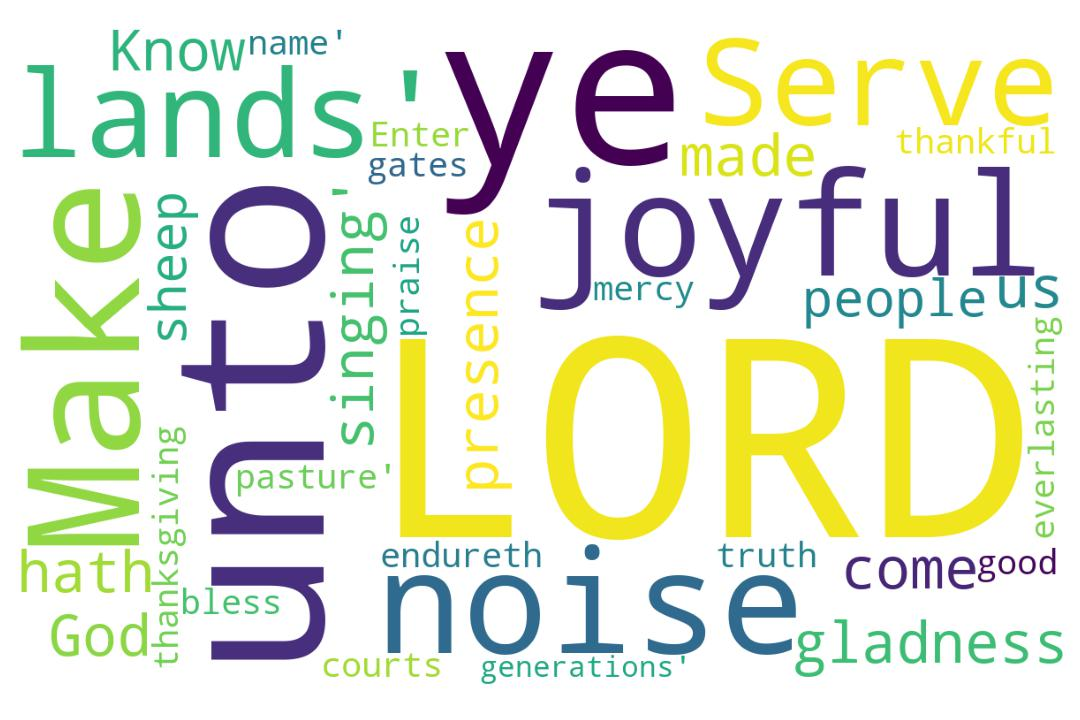
\includegraphics[width=\linewidth]{19OT-Psalms/Psalm100-WordCloud.jpg}
  \caption{Psalm 100 Word Cloud}
  \label{fig:Psalm 100 word Cloud}
\end{figure}


\marginpar{\scriptsize \centering \fcolorbox{bone}{lime}{\textbf{BECAUSE GOD IS GOOD}}\\ (Psalm 100:1-5)

\begin{compactenum}[I.][8]
    \item The \textbf{Geography} of Praise \index[scripture]{Psalms!Psa 100:01} (Psa 100:1)
    \item The \textbf{Gladness} of Praise \index[scripture]{Psalms!Psa 100:02} (Psa 100:2)
    \item Like \textbf{Grazing} Sheep \index[scripture]{Psalms!Psa 100:03} (Psa 100:3)
    \item The \textbf{Gates} of Thanksgiving \index[scripture]{Psalms!Psa 100:04} (Psa 100:4)
    \item The \textbf{Gladness} \index[scripture]{Psalms!Psa 100:02} (Psa 100:2)
    \item The \textbf{Gratitude} \index[scripture]{Psalms!Psa 100:02} (Psa 100:2)
    \item All \textbf{Generations} \index[scripture]{Psalms!Psa 100:05} (Psa 100:5)
    \item Because He is \textbf{Good} \index[scripture]{Psalms!Psa 100:05} (Psa 100:5)
\end{compactenum}}




\footnote{\textcolor[rgb]{0.00,0.25,0.00}{\hyperlink{TOC}{Return to end of Table of Contents.}}}\footnote{\href{https://audiobible.com/bible/psalms_100.html}{\textcolor[cmyk]{0.99998,1,0,0}{Psalm 100 Audio}}}\textcolor[cmyk]{0.99998,1,0,0}{A Psalm of praise.}\\
\\
\textcolor[cmyk]{0.99998,1,0,0}{Make a joyful noise unto the LORD, \fcolorbox{bone}{lime}{all ye lands}.}
[2] \textcolor[cmyk]{0.99998,1,0,0}{Serve the LORD with \fcolorbox{bone}{lime}{gladness}: come before his presence with singing.}
[3] \textcolor[cmyk]{0.99998,1,0,0}{Know ye that the LORD he \emph{is} God: \emph{it} \emph{is} he \emph{that} hath made us, and not we ourselves; \emph{we} \emph{are} his people, and the \fcolorbox{bone}{lime}{sheep of his pasture}.}
[4] \textcolor[cmyk]{0.99998,1,0,0}{Enter into his \fcolorbox{bone}{lime}{gates with thanksgiving}, \emph{and} into his courts with praise: be thankful unto him, \emph{and} bless his name.}
[5] \textcolor[cmyk]{0.99998,1,0,0}{For the LORD \emph{is} \fcolorbox{bone}{lime}{good}; his mercy \emph{is} everlasting; and his truth \emph{endureth} to all \fcolorbox{bone}{lime}{generations}.}
\index[NWIV]{10!Psalm!Psa 100:1}\index[AWIP]{Make!Psalm!Psa 100:1}\index[AWIP]{a!Psalm!Psa 100:1}\index[AWIP]{joyful!Psalm!Psa 100:1}\index[AWIP]{noise!Psalm!Psa 100:1}\index[AWIP]{unto!Psalm!Psa 100:1}\index[AWIP]{the!Psalm!Psa 100:1}\index[AWIP]{LORD!Psalm!Psa 100:1}\index[AWIP]{all!Psalm!Psa 100:1}\index[AWIP]{ye!Psalm!Psa 100:1}\index[AWIP]{lands!Psalm!Psa 100:1}

\index[NWIV]{11!Psalm!Psa 100:2}\index[AWIP]{Serve!Psalm!Psa 100:2}\index[AWIP]{the!Psalm!Psa 100:2}\index[AWIP]{LORD!Psalm!Psa 100:2}\index[AWIP]{with!Psalm!Psa 100:2}\index[AWIP]{with!Psalm!Psa 100:2 (2)}\index[AWIP]{gladness!Psalm!Psa 100:2}\index[AWIP]{come!Psalm!Psa 100:2}\index[AWIP]{before!Psalm!Psa 100:2}\index[AWIP]{his!Psalm!Psa 100:2}\index[AWIP]{presence!Psalm!Psa 100:2}\index[AWIP]{singing!Psalm!Psa 100:2}

\index[NWIV]{29!Psalm!Psa 100:3}\index[AWIP]{Know!Psalm!Psa 100:3}\index[AWIP]{ye!Psalm!Psa 100:3}\index[AWIP]{that!Psalm!Psa 100:3}\index[AWIP]{the!Psalm!Psa 100:3}\index[AWIP]{the!Psalm!Psa 100:3 (2)}\index[AWIP]{LORD!Psalm!Psa 100:3}\index[AWIP]{he!Psalm!Psa 100:3}\index[AWIP]{he!Psalm!Psa 100:3 (2)}\index[AWIP]{\emph{is}!Psalm!Psa 100:3}\index[AWIP]{\emph{is}!Psalm!Psa 100:3 (2)}\index[AWIP]{God!Psalm!Psa 100:3}\index[AWIP]{\emph{it}!Psalm!Psa 100:3}\index[AWIP]{\emph{that}!Psalm!Psa 100:3}\index[AWIP]{hath!Psalm!Psa 100:3}\index[AWIP]{made!Psalm!Psa 100:3}\index[AWIP]{us!Psalm!Psa 100:3}\index[AWIP]{and!Psalm!Psa 100:3}\index[AWIP]{and!Psalm!Psa 100:3 (2)}\index[AWIP]{not!Psalm!Psa 100:3}\index[AWIP]{we!Psalm!Psa 100:3}\index[AWIP]{ourselves!Psalm!Psa 100:3}\index[AWIP]{\emph{we}!Psalm!Psa 100:3}\index[AWIP]{\emph{are}!Psalm!Psa 100:3}\index[AWIP]{his!Psalm!Psa 100:3}\index[AWIP]{his!Psalm!Psa 100:3 (2)}\index[AWIP]{people!Psalm!Psa 100:3}\index[AWIP]{sheep!Psalm!Psa 100:3}\index[AWIP]{of!Psalm!Psa 100:3}\index[AWIP]{pasture!Psalm!Psa 100:3}\index[AWIP]{\emph{is}!Psalm!Psa 100:3}\index[AWIP]{\emph{is}!Psalm!Psa 100:3 (2)}\index[AWIP]{\emph{it}!Psalm!Psa 100:3}\index[AWIP]{\emph{that}!Psalm!Psa 100:3}\index[AWIP]{\emph{we}!Psalm!Psa 100:3}\index[AWIP]{\emph{are}!Psalm!Psa 100:3}

\index[NWIV]{20!Psalm!Psa 100:4}\index[AWIP]{Enter!Psalm!Psa 100:4}\index[AWIP]{into!Psalm!Psa 100:4}\index[AWIP]{into!Psalm!Psa 100:4 (2)}\index[AWIP]{his!Psalm!Psa 100:4}\index[AWIP]{his!Psalm!Psa 100:4 (2)}\index[AWIP]{his!Psalm!Psa 100:4 (3)}\index[AWIP]{gates!Psalm!Psa 100:4}\index[AWIP]{with!Psalm!Psa 100:4}\index[AWIP]{with!Psalm!Psa 100:4 (2)}\index[AWIP]{thanksgiving!Psalm!Psa 100:4}\index[AWIP]{\emph{and}!Psalm!Psa 100:4}\index[AWIP]{\emph{and}!Psalm!Psa 100:4 (2)}\index[AWIP]{courts!Psalm!Psa 100:4}\index[AWIP]{praise!Psalm!Psa 100:4}\index[AWIP]{be!Psalm!Psa 100:4}\index[AWIP]{thankful!Psalm!Psa 100:4}\index[AWIP]{unto!Psalm!Psa 100:4}\index[AWIP]{him!Psalm!Psa 100:4}\index[AWIP]{bless!Psalm!Psa 100:4}\index[AWIP]{name!Psalm!Psa 100:4}\index[AWIP]{\emph{and}!Psalm!Psa 100:4}\index[AWIP]{\emph{and}!Psalm!Psa 100:4 (2)}

\index[NWIV]{16!Psalm!Psa 100:5}\index[AWIP]{For!Psalm!Psa 100:5}\index[AWIP]{the!Psalm!Psa 100:5}\index[AWIP]{LORD!Psalm!Psa 100:5}\index[AWIP]{\emph{is}!Psalm!Psa 100:5}\index[AWIP]{\emph{is}!Psalm!Psa 100:5 (2)}\index[AWIP]{good!Psalm!Psa 100:5}\index[AWIP]{his!Psalm!Psa 100:5}\index[AWIP]{his!Psalm!Psa 100:5 (2)}\index[AWIP]{mercy!Psalm!Psa 100:5}\index[AWIP]{everlasting!Psalm!Psa 100:5}\index[AWIP]{and!Psalm!Psa 100:5}\index[AWIP]{truth!Psalm!Psa 100:5}\index[AWIP]{\emph{endureth}!Psalm!Psa 100:5}\index[AWIP]{to!Psalm!Psa 100:5}\index[AWIP]{all!Psalm!Psa 100:5}\index[AWIP]{generations!Psalm!Psa 100:5}\index[AWIP]{\emph{is}!Psalm!Psa 100:5}\index[AWIP]{\emph{is}!Psalm!Psa 100:5 (2)}\index[AWIP]{\emph{endureth}!Psalm!Psa 100:5}


\section{Psalm 100 Outlines}

\subsection{My Outlines}

\subsubsection{Because God is Good}

\index[speaker]{Keith Anthony!Psalm 100 (Because God is Good)}
\index[series]{Psalms (Keith Anthony)!Psalm 100 (Because God is Good)}
\index[date]{2017/09/02!Psalm 100 (Because God is Good) (Keith Anthony)}

\begin{compactenum}[I.]
    \item The \textbf{Geography} of Praise \index[scripture]{Psalms!Psa 100:01} (Psa 100:1)
    \item The \textbf{Gladness} of Praise \index[scripture]{Psalms!Psa 100:02} (Psa 100:2)
    \item Like \textbf{Grazing} Sheep \index[scripture]{Psalms!Psa 100:03} (Psa 100:3)
    \item The \textbf{Gates} of Thanksgiving \index[scripture]{Psalms!Psa 100:04} (Psa 100:4)
    \item The \textbf{Gratitude} \index[scripture]{Psalms!Psa 100:02} (Psa 100:2)
    \item All \textbf{Generations} \index[scripture]{Psalms!Psa 100:05} (Psa 100:5)
    \item Because He is \textbf{Good} \index[scripture]{Psalms!Psa 100:05} (Psa 100:5)
\end{compactenum}


%\subsection{Outlines from Others}


\section{Psalm 100 Comments}





\chapter{Proverb 10}

\begin{figure}
  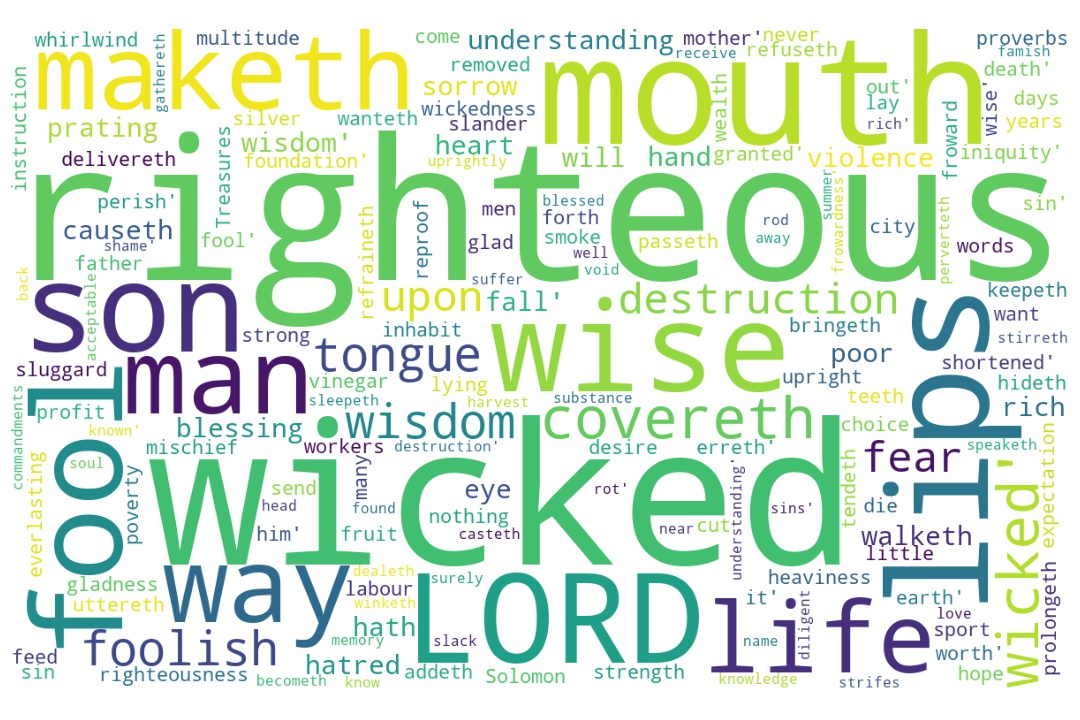
\includegraphics[width=\linewidth]{20OT-Proverbs/Proverb10-WordCloud.jpg}
  \caption{Proverb 10 Word Cloud}
  \label{fig:Proverb 10 Word Cloud}
\end{figure}

\marginpar{\scriptsize \centering\fcolorbox{bone}{lime}{\textbf{THE RIGHTEOUS \& WICKED}}\\ (Proverb 10:1-32)
\begin{compactenum}[I.][8]
	\item \textbf{Shame to the Lazy}  \index[scripture]{Proverbs!Pro 10:05} (Pro 10:5)
	\item \textbf{Sure Footing for the Upright}  \index[scripture]{Proverbs!Pro 10:09} (Pro 10:9)
	\item \textbf{Strife to the Hateful}  \index[scripture]{Proverbs!Pro 10:12} (Pro 10:12)
	\item More \textbf{Sin for the Wicked}  \index[scripture]{Proverbs!Pro 10:16} (Pro 10:16)
	\item \textbf{Sustenance form the Righteous}  \index[scripture]{Proverbs!Pro 10:21} (Pro 10:21)
	\item \textbf{Stinging Eyes to the Sluggard}  \index[scripture]{Proverbs!Pro 10:26} (Pro 10:26)
	\item \textbf{Strength to the Upright} \index[scripture]{Proverbs!Pro 10:29} (Pro 10:29)
\end{compactenum}}

\marginpar{\scriptsize \centering\fcolorbox{bone}{yellow}{\textbf{7 THINGS OF LIFE}}\\ (Proverb 10:1-32)
    \begin{compactenum}[I.][8]
	\item The \textbf{Well} of Life \index[scripture]{Proverbs!Pro 10:11} (Pro 10:11)
	
	\item A \textbf{Wellspring} of Life \index[scripture]{Proverbs!Pro 16:22} \index[scripture]{Proverbs!Pro 18:4} (Pro 16:22, 18:4)
	
	\item The \textbf{way} of Life \index[scripture]{Pro!Pro 06:23} \index[scripture]{Pro!Pro 10:17} \index[scripture]{Pro!Pro 15:24} \index[scripture]{Jer!Jer 21:8} (Pro 6:23, 10:17, 15:24, Jer 21:8)

	\item The \textbf{ways} of Life \index[scripture]{Acts!Acts 02:28} (Acts 2:28)
	
	\item The \textbf{water} of Life \index[scripture]{Rev!Rev 21:06} \index[scripture]{Rev!Rev 22:01} \index[scripture]{Rev!Rev 22:17}  (Rev 21:6, 22:1, 22:17)
	
	\item The \textbf{word} of Life \index[scripture]{Phil!Phil 02:16} (Phil 2:16)
	
	\item The \textbf{Word} of Life \index[scripture]{1Jn!1Jn 1:1}  (1 John 1:1)
\end{compactenum}}

\footnote{\textcolor[cmyk]{0.99998,1,0,0}{\hyperlink{TOC}{Return to end of Table of Contents.}}}\footnote{\href{https://audiobible.com/bible/proverbs_10.html}{\textcolor[cmyk]{0.99998,1,0,0}{Proverbs Audio}}}\textcolor[cmyk]{0.99998,1,0,0}{The proverbs of Solomon. A wise son maketh a glad father: but a foolish son \emph{is} the heaviness of his mother.}
[2] \textcolor[cmyk]{0.99998,1,0,0}{Treasures of wickedness profit nothing: but \fcolorbox{bone}{MYGOLD}{righteousness} delivereth from death.}
[3] \textcolor[cmyk]{0.99998,1,0,0}{The LORD will not suffer the soul of the righteous to famish: but he casteth away the substance of the wicked.}\footnote{\textbf{Psalm 37:25} - I have been young, and now am old; yet have I not seen the righteous forsaken, nor his seed begging bread.}
[4] \textcolor[cmyk]{0.99998,1,0,0}{He becometh poor that dealeth \emph{with} a slack hand: but the hand of the diligent maketh rich.}
[5] \textcolor[cmyk]{0.99998,1,0,0}{He that gathereth in summer \emph{is} a wise son: \emph{but} he that sleepeth in harvest \emph{is} a son that causeth \fcolorbox{bone}{lime}{shame}.}
[6] \textcolor[cmyk]{0.99998,1,0,0}{Blessings \emph{are} upon the head of the just: but violence covereth the mouth of the wicked.}
[7] \textcolor[cmyk]{0.99998,1,0,0}{The memory of the just \emph{is} blessed: but the name of the wicked shall rot.}
[8] \textcolor[cmyk]{0.99998,1,0,0}{Thewise in heart will receive commandments: but a prating fool shall fall.}
[9] \textcolor[cmyk]{0.99998,1,0,0}{He that walketh uprightly walketh \fcolorbox{bone}{lime}{surely}: but he that perverteth his ways shall be known.}
[10] \textcolor[cmyk]{0.99998,1,0,0}{He that winketh with the eye causeth sorrow: but a prating fool shall fall.}\footnote{\textbf{Proverbs 6:13} - He winketh with his eyes, he speaketh with his feet, he teacheth with his fingers;} 
[11] \textcolor[cmyk]{0.99998,1,0,0}{The mouth of a righteous \emph{man} \emph{is} a well of life: but violence covereth the mouth of the wicked.}\footnote{\textbf{Proverb 16:22} - Understanding is a wellspring of life unto him that hath it: but the instruction of fools is folly.}
[12] \textcolor[cmyk]{0.99998,1,0,0}{Hatred stirreth up \fcolorbox{bone}{lime}{strifes}: but love covereth all sins.}
[13] \textcolor[cmyk]{0.99998,1,0,0}{In  the lips of him that hath \fcolorbox{bone}{MYGOLD}{understanding} wisdom is found: but a rod \emph{is} for the back of him that is void of \fcolorbox{bone}{MYGOLD}{understanding}.}
[14] \textcolor[cmyk]{0.99998,1,0,0}{Wise  \emph{men} lay up knowledge: but the mouth of the foolish \emph{is} near destruction.}
[15] \textcolor[cmyk]{0.99998,1,0,0}{The  rich man's wealth \emph{is} his strong city: the destruction of the poor \emph{is} their poverty.}
[16] \textcolor[cmyk]{0.99998,1,0,0}{The  labour of the righteous \emph{tendeth} to life: the fruit of the wicked \fcolorbox{bone}{lime}{to sin}.}
[17] \textcolor[cmyk]{0.99998,1,0,0}{He  \emph{is} \emph{in} the way of life that keepeth instruction: but he that refuseth reproof erreth.}
[18] \textcolor[cmyk]{0.99998,1,0,0}{He  that hideth hatred \emph{with} lying lips, and he that uttereth a slander, \emph{is} a fool.}
[19] \textcolor[cmyk]{0.99998,1,0,0}{In  the multitude of words there wanteth not sin: but he that refraineth his lips \emph{is} wise.}
[20] \textcolor[cmyk]{0.99998,1,0,0}{The tongue of the just \emph{is} \emph{as} choice silver: the heart of the wicked \emph{is} little worth.}
[21] \textcolor[cmyk]{0.99998,1,0,0}{The lips of the righteous \fcolorbox{bone}{lime}{feed many}: but fools die for want of wisdom.}
[22] \textcolor[cmyk]{0.99998,1,0,0}{The blessing of the LORD, it maketh rich, and he addeth no sorrow with it.}
[23] \textcolor[cmyk]{0.99998,1,0,0}{\emph{It} \emph{is} as sport to a fool to do mischief: but a man of \fcolorbox{bone}{MYGOLD}{understanding} hath wisdom.}
[24] \textcolor[cmyk]{0.99998,1,0,0}{The fear of the wicked, it shall come upon him: but the desire of the righteous shall be granted.}
[25] \textcolor[cmyk]{0.99998,1,0,0}{As the whirlwind passeth, so \emph{is} the wicked no \emph{more}: but the righteous \emph{is} an everlasting foundation.}
[26] \textcolor[cmyk]{0.99998,1,0,0}{As vinegar to the teeth, and as \fcolorbox{bone}{lime}{smoke to the eyes}, so \emph{is} the sluggard to them that send him.}
[27] \textcolor[cmyk]{0.99998,1,0,0}{The fear of the LORD prolongeth days: but the years of the wicked shall be shortened.}
[28] \textcolor[cmyk]{0.99998,1,0,0}{The hope of the righteous \emph{shall} \emph{be} gladness: but the expectation of the wicked shall perish.}
[29] \textcolor[cmyk]{0.99998,1,0,0}{The way of the LORD \emph{is} \fcolorbox{bone}{lime}{strength to the upright}: but destruction \emph{shall} \emph{be} to the workers of iniquity.}
[30] \textcolor[cmyk]{0.99998,1,0,0}{The righteous shall never be removed: but the wicked shall not inhabit the earth.}
[31] \textcolor[cmyk]{0.99998,1,0,0}{The mouth of the just bringeth forth wisdom: but the froward tongue shall be cut out.}
[32] \textcolor[cmyk]{0.99998,1,0,0}{The lips of the righteous know what is acceptable: but the mouth of the wicked \emph{speaketh} frowardness.}


\index[NWIV]{21!Proverbs!Pro 10:1}\index[AWIP]{The!Proverbs!Pro 10:1}\index[AWIP]{proverbs!Proverbs!Pro 10:1}\index[AWIP]{of!Proverbs!Pro 10:1}\index[AWIP]{of!Proverbs!Pro 10:1 (2)}\index[AWIP]{Solomon!Proverbs!Pro 10:1}\index[AWIP]{A!Proverbs!Pro 10:1}\index[AWIP]{wise!Proverbs!Pro 10:1}\index[AWIP]{son!Proverbs!Pro 10:1}\index[AWIP]{son!Proverbs!Pro 10:1 (2)}\index[AWIP]{maketh!Proverbs!Pro 10:1}\index[AWIP]{a!Proverbs!Pro 10:1}\index[AWIP]{a!Proverbs!Pro 10:1 (2)}\index[AWIP]{glad!Proverbs!Pro 10:1}\index[AWIP]{father!Proverbs!Pro 10:1}\index[AWIP]{but!Proverbs!Pro 10:1}\index[AWIP]{foolish!Proverbs!Pro 10:1}\index[AWIP]{\emph{is}!Proverbs!Pro 10:1}\index[AWIP]{the!Proverbs!Pro 10:1}\index[AWIP]{heaviness!Proverbs!Pro 10:1}\index[AWIP]{his!Proverbs!Pro 10:1}\index[AWIP]{mother!Proverbs!Pro 10:1}\index[AWIP]{\emph{is}!Proverbs!Pro 10:1}

\index[NWIV]{10!Proverbs!Pro 10:2}\index[AWIP]{Treasures!Proverbs!Pro 10:2}\index[AWIP]{of!Proverbs!Pro 10:2}\index[AWIP]{wickedness!Proverbs!Pro 10:2}\index[AWIP]{profit!Proverbs!Pro 10:2}\index[AWIP]{nothing!Proverbs!Pro 10:2}\index[AWIP]{but!Proverbs!Pro 10:2}\index[AWIP]{righteousness!Proverbs!Pro 10:2}\index[AWIP]{delivereth!Proverbs!Pro 10:2}\index[AWIP]{from!Proverbs!Pro 10:2}\index[AWIP]{death!Proverbs!Pro 10:2}

\index[NWIV]{21!Proverbs!Pro 10:3}\index[AWIP]{The!Proverbs!Pro 10:3}\index[AWIP]{LORD!Proverbs!Pro 10:3}\index[AWIP]{will!Proverbs!Pro 10:3}\index[AWIP]{not!Proverbs!Pro 10:3}\index[AWIP]{suffer!Proverbs!Pro 10:3}\index[AWIP]{the!Proverbs!Pro 10:3}\index[AWIP]{the!Proverbs!Pro 10:3 (2)}\index[AWIP]{the!Proverbs!Pro 10:3 (3)}\index[AWIP]{the!Proverbs!Pro 10:3 (4)}\index[AWIP]{soul!Proverbs!Pro 10:3}\index[AWIP]{of!Proverbs!Pro 10:3}\index[AWIP]{of!Proverbs!Pro 10:3 (2)}\index[AWIP]{righteous!Proverbs!Pro 10:3}\index[AWIP]{to!Proverbs!Pro 10:3}\index[AWIP]{famish!Proverbs!Pro 10:3}\index[AWIP]{but!Proverbs!Pro 10:3}\index[AWIP]{he!Proverbs!Pro 10:3}\index[AWIP]{casteth!Proverbs!Pro 10:3}\index[AWIP]{away!Proverbs!Pro 10:3}\index[AWIP]{substance!Proverbs!Pro 10:3}\index[AWIP]{wicked!Proverbs!Pro 10:3}

\index[NWIV]{17!Proverbs!Pro 10:4}\index[AWIP]{He!Proverbs!Pro 10:4}\index[AWIP]{becometh!Proverbs!Pro 10:4}\index[AWIP]{poor!Proverbs!Pro 10:4}\index[AWIP]{that!Proverbs!Pro 10:4}\index[AWIP]{dealeth!Proverbs!Pro 10:4}\index[AWIP]{\emph{with}!Proverbs!Pro 10:4}\index[AWIP]{a!Proverbs!Pro 10:4}\index[AWIP]{slack!Proverbs!Pro 10:4}\index[AWIP]{hand!Proverbs!Pro 10:4}\index[AWIP]{hand!Proverbs!Pro 10:4 (2)}\index[AWIP]{but!Proverbs!Pro 10:4}\index[AWIP]{the!Proverbs!Pro 10:4}\index[AWIP]{the!Proverbs!Pro 10:4 (2)}\index[AWIP]{of!Proverbs!Pro 10:4}\index[AWIP]{diligent!Proverbs!Pro 10:4}\index[AWIP]{maketh!Proverbs!Pro 10:4}\index[AWIP]{rich!Proverbs!Pro 10:4}\index[AWIP]{\emph{with}!Proverbs!Pro 10:4}

\index[NWIV]{21!Proverbs!Pro 10:5}\index[AWIP]{He!Proverbs!Pro 10:5}\index[AWIP]{that!Proverbs!Pro 10:5}\index[AWIP]{that!Proverbs!Pro 10:5 (2)}\index[AWIP]{that!Proverbs!Pro 10:5 (3)}\index[AWIP]{gathereth!Proverbs!Pro 10:5}\index[AWIP]{in!Proverbs!Pro 10:5}\index[AWIP]{in!Proverbs!Pro 10:5 (2)}\index[AWIP]{summer!Proverbs!Pro 10:5}\index[AWIP]{\emph{is}!Proverbs!Pro 10:5}\index[AWIP]{\emph{is}!Proverbs!Pro 10:5 (2)}\index[AWIP]{a!Proverbs!Pro 10:5}\index[AWIP]{a!Proverbs!Pro 10:5 (2)}\index[AWIP]{wise!Proverbs!Pro 10:5}\index[AWIP]{son!Proverbs!Pro 10:5}\index[AWIP]{son!Proverbs!Pro 10:5 (2)}\index[AWIP]{\emph{but}!Proverbs!Pro 10:5}\index[AWIP]{he!Proverbs!Pro 10:5}\index[AWIP]{sleepeth!Proverbs!Pro 10:5}\index[AWIP]{harvest!Proverbs!Pro 10:5}\index[AWIP]{causeth!Proverbs!Pro 10:5}\index[AWIP]{shame!Proverbs!Pro 10:5}\index[AWIP]{\emph{is}!Proverbs!Pro 10:5}\index[AWIP]{\emph{is}!Proverbs!Pro 10:5 (2)}\index[AWIP]{\emph{but}!Proverbs!Pro 10:5}

\index[NWIV]{16!Proverbs!Pro 10:6}\index[AWIP]{Blessings!Proverbs!Pro 10:6}\index[AWIP]{\emph{are}!Proverbs!Pro 10:6}\index[AWIP]{upon!Proverbs!Pro 10:6}\index[AWIP]{the!Proverbs!Pro 10:6}\index[AWIP]{the!Proverbs!Pro 10:6 (2)}\index[AWIP]{the!Proverbs!Pro 10:6 (3)}\index[AWIP]{the!Proverbs!Pro 10:6 (4)}\index[AWIP]{head!Proverbs!Pro 10:6}\index[AWIP]{of!Proverbs!Pro 10:6}\index[AWIP]{of!Proverbs!Pro 10:6 (2)}\index[AWIP]{just!Proverbs!Pro 10:6}\index[AWIP]{but!Proverbs!Pro 10:6}\index[AWIP]{violence!Proverbs!Pro 10:6}\index[AWIP]{covereth!Proverbs!Pro 10:6}\index[AWIP]{mouth!Proverbs!Pro 10:6}\index[AWIP]{wicked!Proverbs!Pro 10:6}\index[AWIP]{\emph{are}!Proverbs!Pro 10:6}

\index[NWIV]{15!Proverbs!Pro 10:7}\index[AWIP]{The!Proverbs!Pro 10:7}\index[AWIP]{memory!Proverbs!Pro 10:7}\index[AWIP]{of!Proverbs!Pro 10:7}\index[AWIP]{of!Proverbs!Pro 10:7 (2)}\index[AWIP]{the!Proverbs!Pro 10:7}\index[AWIP]{the!Proverbs!Pro 10:7 (2)}\index[AWIP]{the!Proverbs!Pro 10:7 (3)}\index[AWIP]{just!Proverbs!Pro 10:7}\index[AWIP]{\emph{is}!Proverbs!Pro 10:7}\index[AWIP]{blessed!Proverbs!Pro 10:7}\index[AWIP]{but!Proverbs!Pro 10:7}\index[AWIP]{name!Proverbs!Pro 10:7}\index[AWIP]{wicked!Proverbs!Pro 10:7}\index[AWIP]{shall!Proverbs!Pro 10:7}\index[AWIP]{rot!Proverbs!Pro 10:7}\index[AWIP]{\emph{is}!Proverbs!Pro 10:7}

\index[NWIV]{13!Proverbs!Pro 10:8}\index[AWIP]{The!Proverbs!Pro 10:8}\index[AWIP]{wise!Proverbs!Pro 10:8}\index[AWIP]{in!Proverbs!Pro 10:8}\index[AWIP]{heart!Proverbs!Pro 10:8}\index[AWIP]{will!Proverbs!Pro 10:8}\index[AWIP]{receive!Proverbs!Pro 10:8}\index[AWIP]{commandments!Proverbs!Pro 10:8}\index[AWIP]{but!Proverbs!Pro 10:8}\index[AWIP]{a!Proverbs!Pro 10:8}\index[AWIP]{prating!Proverbs!Pro 10:8}\index[AWIP]{fool!Proverbs!Pro 10:8}\index[AWIP]{shall!Proverbs!Pro 10:8}\index[AWIP]{fall!Proverbs!Pro 10:8}

\index[NWIV]{15!Proverbs!Pro 10:9}\index[AWIP]{He!Proverbs!Pro 10:9}\index[AWIP]{that!Proverbs!Pro 10:9}\index[AWIP]{that!Proverbs!Pro 10:9 (2)}\index[AWIP]{walketh!Proverbs!Pro 10:9}\index[AWIP]{walketh!Proverbs!Pro 10:9 (2)}\index[AWIP]{uprightly!Proverbs!Pro 10:9}\index[AWIP]{surely!Proverbs!Pro 10:9}\index[AWIP]{but!Proverbs!Pro 10:9}\index[AWIP]{he!Proverbs!Pro 10:9}\index[AWIP]{perverteth!Proverbs!Pro 10:9}\index[AWIP]{his!Proverbs!Pro 10:9}\index[AWIP]{ways!Proverbs!Pro 10:9}\index[AWIP]{shall!Proverbs!Pro 10:9}\index[AWIP]{be!Proverbs!Pro 10:9}\index[AWIP]{known!Proverbs!Pro 10:9}

\index[NWIV]{14!Proverbs!Pro 10:10}\index[AWIP]{He!Proverbs!Pro 10:10}\index[AWIP]{that!Proverbs!Pro 10:10}\index[AWIP]{winketh!Proverbs!Pro 10:10}\index[AWIP]{with!Proverbs!Pro 10:10}\index[AWIP]{the!Proverbs!Pro 10:10}\index[AWIP]{eye!Proverbs!Pro 10:10}\index[AWIP]{causeth!Proverbs!Pro 10:10}\index[AWIP]{sorrow!Proverbs!Pro 10:10}\index[AWIP]{but!Proverbs!Pro 10:10}\index[AWIP]{a!Proverbs!Pro 10:10}\index[AWIP]{prating!Proverbs!Pro 10:10}\index[AWIP]{fool!Proverbs!Pro 10:10}\index[AWIP]{shall!Proverbs!Pro 10:10}\index[AWIP]{fall!Proverbs!Pro 10:10}

\index[NWIV]{19!Proverbs!Pro 10:11}\index[AWIP]{The!Proverbs!Pro 10:11}\index[AWIP]{mouth!Proverbs!Pro 10:11}\index[AWIP]{mouth!Proverbs!Pro 10:11 (2)}\index[AWIP]{of!Proverbs!Pro 10:11}\index[AWIP]{of!Proverbs!Pro 10:11 (2)}\index[AWIP]{of!Proverbs!Pro 10:11 (3)}\index[AWIP]{a!Proverbs!Pro 10:11}\index[AWIP]{a!Proverbs!Pro 10:11 (2)}\index[AWIP]{righteous!Proverbs!Pro 10:11}\index[AWIP]{\emph{man}!Proverbs!Pro 10:11}\index[AWIP]{\emph{is}!Proverbs!Pro 10:11}\index[AWIP]{well!Proverbs!Pro 10:11}\index[AWIP]{life!Proverbs!Pro 10:11}\index[AWIP]{but!Proverbs!Pro 10:11}\index[AWIP]{violence!Proverbs!Pro 10:11}\index[AWIP]{covereth!Proverbs!Pro 10:11}\index[AWIP]{the!Proverbs!Pro 10:11}\index[AWIP]{the!Proverbs!Pro 10:11 (2)}\index[AWIP]{wicked!Proverbs!Pro 10:11}\index[AWIP]{\emph{man}!Proverbs!Pro 10:11}\index[AWIP]{\emph{is}!Proverbs!Pro 10:11}

\index[NWIV]{9!Proverbs!Pro 10:12}\index[AWIP]{Hatred!Proverbs!Pro 10:12}\index[AWIP]{stirreth!Proverbs!Pro 10:12}\index[AWIP]{up!Proverbs!Pro 10:12}\index[AWIP]{strifes!Proverbs!Pro 10:12}\index[AWIP]{but!Proverbs!Pro 10:12}\index[AWIP]{love!Proverbs!Pro 10:12}\index[AWIP]{covereth!Proverbs!Pro 10:12}\index[AWIP]{all!Proverbs!Pro 10:12}\index[AWIP]{sins!Proverbs!Pro 10:12}

\index[NWIV]{25!Proverbs!Pro 10:13}\index[AWIP]{In!Proverbs!Pro 10:13}\index[AWIP]{the!Proverbs!Pro 10:13}\index[AWIP]{the!Proverbs!Pro 10:13 (2)}\index[AWIP]{lips!Proverbs!Pro 10:13}\index[AWIP]{of!Proverbs!Pro 10:13}\index[AWIP]{of!Proverbs!Pro 10:13 (2)}\index[AWIP]{of!Proverbs!Pro 10:13 (3)}\index[AWIP]{him!Proverbs!Pro 10:13}\index[AWIP]{him!Proverbs!Pro 10:13 (2)}\index[AWIP]{that!Proverbs!Pro 10:13}\index[AWIP]{that!Proverbs!Pro 10:13 (2)}\index[AWIP]{hath!Proverbs!Pro 10:13}\index[AWIP]{understanding!Proverbs!Pro 10:13}\index[AWIP]{understanding!Proverbs!Pro 10:13 (2)}\index[AWIP]{wisdom!Proverbs!Pro 10:13}\index[AWIP]{is!Proverbs!Pro 10:13}\index[AWIP]{is!Proverbs!Pro 10:13 (2)}\index[AWIP]{found!Proverbs!Pro 10:13}\index[AWIP]{but!Proverbs!Pro 10:13}\index[AWIP]{a!Proverbs!Pro 10:13}\index[AWIP]{rod!Proverbs!Pro 10:13}\index[AWIP]{\emph{is}!Proverbs!Pro 10:13}\index[AWIP]{for!Proverbs!Pro 10:13}\index[AWIP]{back!Proverbs!Pro 10:13}\index[AWIP]{void!Proverbs!Pro 10:13}\index[AWIP]{\emph{is}!Proverbs!Pro 10:13}

\index[NWIV]{14!Proverbs!Pro 10:14}\index[AWIP]{Wise!Proverbs!Pro 10:14}\index[AWIP]{\emph{men}!Proverbs!Pro 10:14}\index[AWIP]{lay!Proverbs!Pro 10:14}\index[AWIP]{up!Proverbs!Pro 10:14}\index[AWIP]{knowledge!Proverbs!Pro 10:14}\index[AWIP]{but!Proverbs!Pro 10:14}\index[AWIP]{the!Proverbs!Pro 10:14}\index[AWIP]{the!Proverbs!Pro 10:14 (2)}\index[AWIP]{mouth!Proverbs!Pro 10:14}\index[AWIP]{of!Proverbs!Pro 10:14}\index[AWIP]{foolish!Proverbs!Pro 10:14}\index[AWIP]{\emph{is}!Proverbs!Pro 10:14}\index[AWIP]{near!Proverbs!Pro 10:14}\index[AWIP]{destruction!Proverbs!Pro 10:14}\index[AWIP]{\emph{men}!Proverbs!Pro 10:14}\index[AWIP]{\emph{is}!Proverbs!Pro 10:14}

\index[NWIV]{16!Proverbs!Pro 10:15}\index[AWIP]{The!Proverbs!Pro 10:15}\index[AWIP]{rich!Proverbs!Pro 10:15}\index[AWIP]{man's!Proverbs!Pro 10:15}\index[AWIP]{wealth!Proverbs!Pro 10:15}\index[AWIP]{\emph{is}!Proverbs!Pro 10:15}\index[AWIP]{\emph{is}!Proverbs!Pro 10:15 (2)}\index[AWIP]{his!Proverbs!Pro 10:15}\index[AWIP]{strong!Proverbs!Pro 10:15}\index[AWIP]{city!Proverbs!Pro 10:15}\index[AWIP]{the!Proverbs!Pro 10:15}\index[AWIP]{the!Proverbs!Pro 10:15 (2)}\index[AWIP]{destruction!Proverbs!Pro 10:15}\index[AWIP]{of!Proverbs!Pro 10:15}\index[AWIP]{poor!Proverbs!Pro 10:15}\index[AWIP]{their!Proverbs!Pro 10:15}\index[AWIP]{poverty!Proverbs!Pro 10:15}\index[AWIP]{\emph{is}!Proverbs!Pro 10:15}\index[AWIP]{\emph{is}!Proverbs!Pro 10:15 (2)}

\index[NWIV]{15!Proverbs!Pro 10:16}\index[AWIP]{The!Proverbs!Pro 10:16}\index[AWIP]{labour!Proverbs!Pro 10:16}\index[AWIP]{of!Proverbs!Pro 10:16}\index[AWIP]{of!Proverbs!Pro 10:16 (2)}\index[AWIP]{the!Proverbs!Pro 10:16}\index[AWIP]{the!Proverbs!Pro 10:16 (2)}\index[AWIP]{the!Proverbs!Pro 10:16 (3)}\index[AWIP]{righteous!Proverbs!Pro 10:16}\index[AWIP]{\emph{tendeth}!Proverbs!Pro 10:16}\index[AWIP]{to!Proverbs!Pro 10:16}\index[AWIP]{to!Proverbs!Pro 10:16 (2)}\index[AWIP]{life!Proverbs!Pro 10:16}\index[AWIP]{fruit!Proverbs!Pro 10:16}\index[AWIP]{wicked!Proverbs!Pro 10:16}\index[AWIP]{sin!Proverbs!Pro 10:16}\index[AWIP]{\emph{tendeth}!Proverbs!Pro 10:16}

\index[NWIV]{16!Proverbs!Pro 10:17}\index[AWIP]{He!Proverbs!Pro 10:17}\index[AWIP]{\emph{is}!Proverbs!Pro 10:17}\index[AWIP]{\emph{in}!Proverbs!Pro 10:17}\index[AWIP]{the!Proverbs!Pro 10:17}\index[AWIP]{way!Proverbs!Pro 10:17}\index[AWIP]{of!Proverbs!Pro 10:17}\index[AWIP]{life!Proverbs!Pro 10:17}\index[AWIP]{that!Proverbs!Pro 10:17}\index[AWIP]{that!Proverbs!Pro 10:17 (2)}\index[AWIP]{keepeth!Proverbs!Pro 10:17}\index[AWIP]{instruction!Proverbs!Pro 10:17}\index[AWIP]{but!Proverbs!Pro 10:17}\index[AWIP]{he!Proverbs!Pro 10:17}\index[AWIP]{refuseth!Proverbs!Pro 10:17}\index[AWIP]{reproof!Proverbs!Pro 10:17}\index[AWIP]{erreth!Proverbs!Pro 10:17}\index[AWIP]{\emph{is}!Proverbs!Pro 10:17}\index[AWIP]{\emph{in}!Proverbs!Pro 10:17}

\index[NWIV]{16!Proverbs!Pro 10:18}\index[AWIP]{He!Proverbs!Pro 10:18}\index[AWIP]{that!Proverbs!Pro 10:18}\index[AWIP]{that!Proverbs!Pro 10:18 (2)}\index[AWIP]{hideth!Proverbs!Pro 10:18}\index[AWIP]{hatred!Proverbs!Pro 10:18}\index[AWIP]{\emph{with}!Proverbs!Pro 10:18}\index[AWIP]{lying!Proverbs!Pro 10:18}\index[AWIP]{lips!Proverbs!Pro 10:18}\index[AWIP]{and!Proverbs!Pro 10:18}\index[AWIP]{he!Proverbs!Pro 10:18}\index[AWIP]{uttereth!Proverbs!Pro 10:18}\index[AWIP]{a!Proverbs!Pro 10:18}\index[AWIP]{a!Proverbs!Pro 10:18 (2)}\index[AWIP]{slander!Proverbs!Pro 10:18}\index[AWIP]{\emph{is}!Proverbs!Pro 10:18}\index[AWIP]{fool!Proverbs!Pro 10:18}\index[AWIP]{\emph{with}!Proverbs!Pro 10:18}\index[AWIP]{\emph{is}!Proverbs!Pro 10:18}

\index[NWIV]{17!Proverbs!Pro 10:19}\index[AWIP]{In!Proverbs!Pro 10:19}\index[AWIP]{the!Proverbs!Pro 10:19}\index[AWIP]{multitude!Proverbs!Pro 10:19}\index[AWIP]{of!Proverbs!Pro 10:19}\index[AWIP]{words!Proverbs!Pro 10:19}\index[AWIP]{there!Proverbs!Pro 10:19}\index[AWIP]{wanteth!Proverbs!Pro 10:19}\index[AWIP]{not!Proverbs!Pro 10:19}\index[AWIP]{sin!Proverbs!Pro 10:19}\index[AWIP]{but!Proverbs!Pro 10:19}\index[AWIP]{he!Proverbs!Pro 10:19}\index[AWIP]{that!Proverbs!Pro 10:19}\index[AWIP]{refraineth!Proverbs!Pro 10:19}\index[AWIP]{his!Proverbs!Pro 10:19}\index[AWIP]{lips!Proverbs!Pro 10:19}\index[AWIP]{\emph{is}!Proverbs!Pro 10:19}\index[AWIP]{wise!Proverbs!Pro 10:19}\index[AWIP]{\emph{is}!Proverbs!Pro 10:19}

\index[NWIV]{17!Proverbs!Pro 10:20}\index[AWIP]{The!Proverbs!Pro 10:20}\index[AWIP]{tongue!Proverbs!Pro 10:20}\index[AWIP]{of!Proverbs!Pro 10:20}\index[AWIP]{of!Proverbs!Pro 10:20 (2)}\index[AWIP]{the!Proverbs!Pro 10:20}\index[AWIP]{the!Proverbs!Pro 10:20 (2)}\index[AWIP]{the!Proverbs!Pro 10:20 (3)}\index[AWIP]{just!Proverbs!Pro 10:20}\index[AWIP]{\emph{is}!Proverbs!Pro 10:20}\index[AWIP]{\emph{is}!Proverbs!Pro 10:20 (2)}\index[AWIP]{\emph{as}!Proverbs!Pro 10:20}\index[AWIP]{choice!Proverbs!Pro 10:20}\index[AWIP]{silver!Proverbs!Pro 10:20}\index[AWIP]{heart!Proverbs!Pro 10:20}\index[AWIP]{wicked!Proverbs!Pro 10:20}\index[AWIP]{little!Proverbs!Pro 10:20}\index[AWIP]{worth!Proverbs!Pro 10:20}\index[AWIP]{\emph{is}!Proverbs!Pro 10:20}\index[AWIP]{\emph{is}!Proverbs!Pro 10:20 (2)}\index[AWIP]{\emph{as}!Proverbs!Pro 10:20}

\index[NWIV]{14!Proverbs!Pro 10:21}\index[AWIP]{The!Proverbs!Pro 10:21}\index[AWIP]{lips!Proverbs!Pro 10:21}\index[AWIP]{of!Proverbs!Pro 10:21}\index[AWIP]{of!Proverbs!Pro 10:21 (2)}\index[AWIP]{the!Proverbs!Pro 10:21}\index[AWIP]{righteous!Proverbs!Pro 10:21}\index[AWIP]{feed!Proverbs!Pro 10:21}\index[AWIP]{many!Proverbs!Pro 10:21}\index[AWIP]{but!Proverbs!Pro 10:21}\index[AWIP]{fools!Proverbs!Pro 10:21}\index[AWIP]{die!Proverbs!Pro 10:21}\index[AWIP]{for!Proverbs!Pro 10:21}\index[AWIP]{want!Proverbs!Pro 10:21}\index[AWIP]{wisdom!Proverbs!Pro 10:21}

\index[NWIV]{15!Proverbs!Pro 10:22}\index[AWIP]{The!Proverbs!Pro 10:22}\index[AWIP]{blessing!Proverbs!Pro 10:22}\index[AWIP]{of!Proverbs!Pro 10:22}\index[AWIP]{the!Proverbs!Pro 10:22}\index[AWIP]{LORD!Proverbs!Pro 10:22}\index[AWIP]{it!Proverbs!Pro 10:22}\index[AWIP]{it!Proverbs!Pro 10:22 (2)}\index[AWIP]{maketh!Proverbs!Pro 10:22}\index[AWIP]{rich!Proverbs!Pro 10:22}\index[AWIP]{and!Proverbs!Pro 10:22}\index[AWIP]{he!Proverbs!Pro 10:22}\index[AWIP]{addeth!Proverbs!Pro 10:22}\index[AWIP]{no!Proverbs!Pro 10:22}\index[AWIP]{sorrow!Proverbs!Pro 10:22}\index[AWIP]{with!Proverbs!Pro 10:22}

\index[NWIV]{17!Proverbs!Pro 10:23}\index[AWIP]{\emph{It}!Proverbs!Pro 10:23}\index[AWIP]{\emph{is}!Proverbs!Pro 10:23}\index[AWIP]{as!Proverbs!Pro 10:23}\index[AWIP]{sport!Proverbs!Pro 10:23}\index[AWIP]{to!Proverbs!Pro 10:23}\index[AWIP]{to!Proverbs!Pro 10:23 (2)}\index[AWIP]{a!Proverbs!Pro 10:23}\index[AWIP]{a!Proverbs!Pro 10:23 (2)}\index[AWIP]{fool!Proverbs!Pro 10:23}\index[AWIP]{do!Proverbs!Pro 10:23}\index[AWIP]{mischief!Proverbs!Pro 10:23}\index[AWIP]{but!Proverbs!Pro 10:23}\index[AWIP]{man!Proverbs!Pro 10:23}\index[AWIP]{of!Proverbs!Pro 10:23}\index[AWIP]{understanding!Proverbs!Pro 10:23}\index[AWIP]{hath!Proverbs!Pro 10:23}\index[AWIP]{wisdom!Proverbs!Pro 10:23}\index[AWIP]{\emph{It}!Proverbs!Pro 10:23}\index[AWIP]{\emph{is}!Proverbs!Pro 10:23}

\index[NWIV]{19!Proverbs!Pro 10:24}\index[AWIP]{The!Proverbs!Pro 10:24}\index[AWIP]{fear!Proverbs!Pro 10:24}\index[AWIP]{of!Proverbs!Pro 10:24}\index[AWIP]{of!Proverbs!Pro 10:24 (2)}\index[AWIP]{the!Proverbs!Pro 10:24}\index[AWIP]{the!Proverbs!Pro 10:24 (2)}\index[AWIP]{the!Proverbs!Pro 10:24 (3)}\index[AWIP]{wicked!Proverbs!Pro 10:24}\index[AWIP]{it!Proverbs!Pro 10:24}\index[AWIP]{shall!Proverbs!Pro 10:24}\index[AWIP]{shall!Proverbs!Pro 10:24 (2)}\index[AWIP]{come!Proverbs!Pro 10:24}\index[AWIP]{upon!Proverbs!Pro 10:24}\index[AWIP]{him!Proverbs!Pro 10:24}\index[AWIP]{but!Proverbs!Pro 10:24}\index[AWIP]{desire!Proverbs!Pro 10:24}\index[AWIP]{righteous!Proverbs!Pro 10:24}\index[AWIP]{be!Proverbs!Pro 10:24}\index[AWIP]{granted!Proverbs!Pro 10:24}

\index[NWIV]{17!Proverbs!Pro 10:25}\index[AWIP]{As!Proverbs!Pro 10:25}\index[AWIP]{the!Proverbs!Pro 10:25}\index[AWIP]{the!Proverbs!Pro 10:25 (2)}\index[AWIP]{the!Proverbs!Pro 10:25 (3)}\index[AWIP]{whirlwind!Proverbs!Pro 10:25}\index[AWIP]{passeth!Proverbs!Pro 10:25}\index[AWIP]{so!Proverbs!Pro 10:25}\index[AWIP]{\emph{is}!Proverbs!Pro 10:25}\index[AWIP]{\emph{is}!Proverbs!Pro 10:25 (2)}\index[AWIP]{wicked!Proverbs!Pro 10:25}\index[AWIP]{no!Proverbs!Pro 10:25}\index[AWIP]{\emph{more}!Proverbs!Pro 10:25}\index[AWIP]{but!Proverbs!Pro 10:25}\index[AWIP]{righteous!Proverbs!Pro 10:25}\index[AWIP]{an!Proverbs!Pro 10:25}\index[AWIP]{everlasting!Proverbs!Pro 10:25}\index[AWIP]{foundation!Proverbs!Pro 10:25}\index[AWIP]{\emph{is}!Proverbs!Pro 10:25}\index[AWIP]{\emph{is}!Proverbs!Pro 10:25 (2)}\index[AWIP]{\emph{more}!Proverbs!Pro 10:25}

\index[NWIV]{20!Proverbs!Pro 10:26}\index[AWIP]{As!Proverbs!Pro 10:26}\index[AWIP]{vinegar!Proverbs!Pro 10:26}\index[AWIP]{to!Proverbs!Pro 10:26}\index[AWIP]{to!Proverbs!Pro 10:26 (2)}\index[AWIP]{to!Proverbs!Pro 10:26 (3)}\index[AWIP]{the!Proverbs!Pro 10:26}\index[AWIP]{the!Proverbs!Pro 10:26 (2)}\index[AWIP]{the!Proverbs!Pro 10:26 (3)}\index[AWIP]{teeth!Proverbs!Pro 10:26}\index[AWIP]{and!Proverbs!Pro 10:26}\index[AWIP]{as!Proverbs!Pro 10:26}\index[AWIP]{smoke!Proverbs!Pro 10:26}\index[AWIP]{eyes!Proverbs!Pro 10:26}\index[AWIP]{so!Proverbs!Pro 10:26}\index[AWIP]{\emph{is}!Proverbs!Pro 10:26}\index[AWIP]{sluggard!Proverbs!Pro 10:26}\index[AWIP]{them!Proverbs!Pro 10:26}\index[AWIP]{that!Proverbs!Pro 10:26}\index[AWIP]{send!Proverbs!Pro 10:26}\index[AWIP]{him!Proverbs!Pro 10:26}\index[AWIP]{\emph{is}!Proverbs!Pro 10:26}

\index[NWIV]{16!Proverbs!Pro 10:27}\index[AWIP]{The!Proverbs!Pro 10:27}\index[AWIP]{fear!Proverbs!Pro 10:27}\index[AWIP]{of!Proverbs!Pro 10:27}\index[AWIP]{of!Proverbs!Pro 10:27 (2)}\index[AWIP]{the!Proverbs!Pro 10:27}\index[AWIP]{the!Proverbs!Pro 10:27 (2)}\index[AWIP]{the!Proverbs!Pro 10:27 (3)}\index[AWIP]{LORD!Proverbs!Pro 10:27}\index[AWIP]{prolongeth!Proverbs!Pro 10:27}\index[AWIP]{days!Proverbs!Pro 10:27}\index[AWIP]{but!Proverbs!Pro 10:27}\index[AWIP]{years!Proverbs!Pro 10:27}\index[AWIP]{wicked!Proverbs!Pro 10:27}\index[AWIP]{shall!Proverbs!Pro 10:27}\index[AWIP]{be!Proverbs!Pro 10:27}\index[AWIP]{shortened!Proverbs!Pro 10:27}

\index[NWIV]{16!Proverbs!Pro 10:28}\index[AWIP]{The!Proverbs!Pro 10:28}\index[AWIP]{hope!Proverbs!Pro 10:28}\index[AWIP]{of!Proverbs!Pro 10:28}\index[AWIP]{of!Proverbs!Pro 10:28 (2)}\index[AWIP]{the!Proverbs!Pro 10:28}\index[AWIP]{the!Proverbs!Pro 10:28 (2)}\index[AWIP]{the!Proverbs!Pro 10:28 (3)}\index[AWIP]{righteous!Proverbs!Pro 10:28}\index[AWIP]{\emph{shall}!Proverbs!Pro 10:28}\index[AWIP]{\emph{be}!Proverbs!Pro 10:28}\index[AWIP]{gladness!Proverbs!Pro 10:28}\index[AWIP]{but!Proverbs!Pro 10:28}\index[AWIP]{expectation!Proverbs!Pro 10:28}\index[AWIP]{wicked!Proverbs!Pro 10:28}\index[AWIP]{shall!Proverbs!Pro 10:28}\index[AWIP]{perish!Proverbs!Pro 10:28}\index[AWIP]{\emph{shall}!Proverbs!Pro 10:28}\index[AWIP]{\emph{be}!Proverbs!Pro 10:28}

\index[NWIV]{19!Proverbs!Pro 10:29}\index[AWIP]{The!Proverbs!Pro 10:29}\index[AWIP]{way!Proverbs!Pro 10:29}\index[AWIP]{of!Proverbs!Pro 10:29}\index[AWIP]{of!Proverbs!Pro 10:29 (2)}\index[AWIP]{the!Proverbs!Pro 10:29}\index[AWIP]{the!Proverbs!Pro 10:29 (2)}\index[AWIP]{the!Proverbs!Pro 10:29 (3)}\index[AWIP]{LORD!Proverbs!Pro 10:29}\index[AWIP]{\emph{is}!Proverbs!Pro 10:29}\index[AWIP]{strength!Proverbs!Pro 10:29}\index[AWIP]{to!Proverbs!Pro 10:29}\index[AWIP]{to!Proverbs!Pro 10:29 (2)}\index[AWIP]{upright!Proverbs!Pro 10:29}\index[AWIP]{but!Proverbs!Pro 10:29}\index[AWIP]{destruction!Proverbs!Pro 10:29}\index[AWIP]{\emph{shall}!Proverbs!Pro 10:29}\index[AWIP]{\emph{be}!Proverbs!Pro 10:29}\index[AWIP]{workers!Proverbs!Pro 10:29}\index[AWIP]{iniquity!Proverbs!Pro 10:29}\index[AWIP]{\emph{is}!Proverbs!Pro 10:29}\index[AWIP]{\emph{shall}!Proverbs!Pro 10:29}\index[AWIP]{\emph{be}!Proverbs!Pro 10:29}

\index[NWIV]{14!Proverbs!Pro 10:30}\index[AWIP]{The!Proverbs!Pro 10:30}\index[AWIP]{righteous!Proverbs!Pro 10:30}\index[AWIP]{shall!Proverbs!Pro 10:30}\index[AWIP]{shall!Proverbs!Pro 10:30 (2)}\index[AWIP]{never!Proverbs!Pro 10:30}\index[AWIP]{be!Proverbs!Pro 10:30}\index[AWIP]{removed!Proverbs!Pro 10:30}\index[AWIP]{but!Proverbs!Pro 10:30}\index[AWIP]{the!Proverbs!Pro 10:30}\index[AWIP]{the!Proverbs!Pro 10:30 (2)}\index[AWIP]{wicked!Proverbs!Pro 10:30}\index[AWIP]{not!Proverbs!Pro 10:30}\index[AWIP]{inhabit!Proverbs!Pro 10:30}\index[AWIP]{earth!Proverbs!Pro 10:30}

\index[NWIV]{16!Proverbs!Pro 10:31}\index[AWIP]{The!Proverbs!Pro 10:31}\index[AWIP]{mouth!Proverbs!Pro 10:31}\index[AWIP]{of!Proverbs!Pro 10:31}\index[AWIP]{the!Proverbs!Pro 10:31}\index[AWIP]{the!Proverbs!Pro 10:31 (2)}\index[AWIP]{just!Proverbs!Pro 10:31}\index[AWIP]{bringeth!Proverbs!Pro 10:31}\index[AWIP]{forth!Proverbs!Pro 10:31}\index[AWIP]{wisdom!Proverbs!Pro 10:31}\index[AWIP]{but!Proverbs!Pro 10:31}\index[AWIP]{froward!Proverbs!Pro 10:31}\index[AWIP]{tongue!Proverbs!Pro 10:31}\index[AWIP]{shall!Proverbs!Pro 10:31}\index[AWIP]{be!Proverbs!Pro 10:31}\index[AWIP]{cut!Proverbs!Pro 10:31}\index[AWIP]{out!Proverbs!Pro 10:31}

\index[NWIV]{17!Proverbs!Pro 10:32}\index[AWIP]{The!Proverbs!Pro 10:32}\index[AWIP]{lips!Proverbs!Pro 10:32}\index[AWIP]{of!Proverbs!Pro 10:32}\index[AWIP]{of!Proverbs!Pro 10:32 (2)}\index[AWIP]{the!Proverbs!Pro 10:32}\index[AWIP]{the!Proverbs!Pro 10:32 (2)}\index[AWIP]{the!Proverbs!Pro 10:32 (3)}\index[AWIP]{righteous!Proverbs!Pro 10:32}\index[AWIP]{know!Proverbs!Pro 10:32}\index[AWIP]{what!Proverbs!Pro 10:32}\index[AWIP]{is!Proverbs!Pro 10:32}\index[AWIP]{acceptable!Proverbs!Pro 10:32}\index[AWIP]{but!Proverbs!Pro 10:32}\index[AWIP]{mouth!Proverbs!Pro 10:32}\index[AWIP]{wicked!Proverbs!Pro 10:32}\index[AWIP]{\emph{speaketh}!Proverbs!Pro 10:32}\index[AWIP]{frowardness!Proverbs!Pro 10:32}\index[AWIP]{\emph{speaketh}!Proverbs!Pro 10:32}

%%%%%%%%%%%%%%%%%%%%%%

\index[DOCTRINES]{Practicology - Substance!!Proverbs!Pro 10:02}
\index[DOCTRINES]{Practicology - Substance!!Proverbs!Pro 10:03}


\index[DOCTRINES]{Practicology - Strife!!Proverbs!Pro 10:12}

\index[DOCTRINES]{Practicology - Success!!Proverbs!Pro 10:16}


\index[DOCTRINES]{Practicology - Speech!!Proverbs!Pro 10:21}







\section{Proverbs 10 Outlines}

\subsection{Outlines from Others}

\subsubsection{Comparing the Righteous and Wicked}
\index[speaker]{Keith Anthony!Proverb 10 (Comparing the Righteous and Wicked)}
\index[series]{Proverbs (Keith Anthony)!Pro 10 (Comparing the Righteous and Wicked)}
\index[date]{2016/05/10!Proverb 10 (Comparing the Righteous and Wicked) (Keith Anthony)}
%\textbf{Lineage}: adpated from S. Conway\\
\textbf{Introduction}: Proverbs 10 begins a section of Solomon's proverbs comparing the righteous and wicked. There is:
\begin{compactenum}[I.]
\item \textbf{Shame to the Lazy}  \index[scripture]{Proverbs!Pro 10:05}(Pro 10:5)
\item \textbf{Sure Footing for the Upright}  \index[scripture]{Proverbs!Pro 10:09}(Pro 10:9)
\item \textbf{Strife to the Hateful}  \index[scripture]{Proverbs!Pro 10:12}(Pro 10:12)
\item More \textbf{Sin for the Wicked}  \index[scripture]{Proverbs!Pro 10:16}(Pro 10:16)
\item \textbf{Sustenance form the Righteous}  \index[scripture]{Proverbs!Pro 10:21}(Pro 10:21)
\item \textbf{Stinging Eyes to the Sluggard}  \index[scripture]{Proverbs!Pro 10:26}(Pro 10:26)
\item \textbf{Strength to the Upright} \index[scripture]{Proverbs!Pro 10:29}(Pro 10:29)
\end{compactenum}

% wisdom [1, 5, 19], wicked [2, 3, 6, 7, 11, 16, 20, 24, 25, 27, 28, 30, 32], walk, wink [10], whirlwind [5], way [17, 29], wealth [10], well [10], worth [20]
\subsection{Outlines from Others}


\section{Proverb 10 Comments}

\subsection{Numeric Nuggets}
\textbf{13:} There are 13 words in Proverb 10:8. Verses 8, 9, 14, 20, 21, 27, and 28 have 13 unique words. The 13-letter words in the chapter are ``righteousness'' and ``understanding.''  




%%% For Indexes

%\index[DEVOTIONAL]{TGIF1!Os Hillman (Living for a Cause Greater Than Yourself) - Proverb 19:17!2021/12/21}

%\index[DEVOTIONAL]{TGIF1!Os Hillman (Living for a Cause Greater Than Yourself) - Proverb 19:17!2021/12/21}

















%%% colour: cardinal red - \textcolor[cmyk]{0,0.85,0.70,0.23}{text}


%%%% Example marginpar with a compactenum list --- green color text
%\marginpar{\scriptsize \textcolor[rgb]{0.00,0.545,0.269}{$\rightarrow$7 Abominations: 
%\begin{compactenum}
%	\item A proud look,
%	\item a lying tongue,
%	\item hands that shed innocent blood,
%	\item An heart that deviseth wicked imaginations,
%	\item feet that be swift in running to mischief,
%	\item A false witness that speaketh lies, and
%	\item he that soweth discord among brethren.
%\end{compactenum}}}



%\newpage

%\begin{mdframed}[style=MyFrame]
%\begin{center}
%\begin{longtable}{|p{.5in}|p{3.5in}|}

%\caption[Corruption Alert: Proverbs 18:1]{Corruption Alert: Proverbs 18:1} \label{table:CorruptionProv18:1} \\ 

%\hline  
%\multicolumn{1}{|c|}{\textbf{Version}} & 
%\multicolumn{1}{c|}{\textbf{Corruption}}  \\ \hline 
%\endfirsthead
 
%\multicolumn{2}{c}
%{{\bfseries \tablename\ \thetable{} -- continued from previous page}} \\  \hline  
%\multicolumn{1}{|c|}{\textbf{Version}} & 
%\multicolumn{1}{c|}{\textbf{Corruption}}  \\ \hline 
%\endhead
 
%\hline \multicolumn{2}{|r|}{{Continued on next page}} \\ \hline
%\endfoot 
%\textcolor[rgb]{0.00,0.00,1.00}{AV} & \textcolor[rgb]{0.00,0.00,1.00}{Through desire a man, having separated himself, seeketh \emph{and} intermeddleth with all wisdom.} \\ \hline
%
%ASV &  He that separateth himself seeketh his own desire, And  rageth against all sound wisdom. \\ \hline
%
%CEB &  Unfriendly people look out for themselves; they bicker with sensible people.\\ \hline
%
%ESV & Whoever isolates himself seeks his own desire;  he breaks out against all sound judgment. \\ \hline
%
%NASV &  He who separates himself seeks his own desire, He quarrels against all sound wisdom.\\ \hline
%
%MEV & He who separates himself seeks his own desire; he seeks and quarrels against all wisdom.\\ \hline
%
%NIV &  An unfriendly person pursues selfish ends and against all sound judgment starts quarrels. \\ \hline
%
%NKJV &  A man who isolates himself seeks his own desire; He rages against all wise judgment.\\ \hline
%
%RSV &  He who is estranged seeks pretexts  to break out against all sound judgment.\\ \hline

% \multicolumn{2}{p{4.3in}}{{Modern translations, such as the ASV and others, strike out the first part of the verse, concealing the intent of mankind in genewisdom clearly revealed in scripture. How wonderful is the obfuscated RSV text: ``He who is estranged seeks pretexts.'' What does THAT mean?}} \\ %\hline

%\hline

%\end{longtable}
%\end{center}

%\normalsize 
%\end{mdframed}

%\marginpar{\scriptsize \centering \fcolorbox{black}{lime}{\textbf{OUTIDE THE PLACE OF PROMISE}}\\ (Psalm 137:1--9) 
%\begin{compactenum}[I.][8]
%	\item \textbf{Plight \& Distress} \index[scripture]{Psalms!Psa 137:01} (Psalm 137:1)
%	\item The \textbf{Place Desired} \index[scripture]{Psalms!Psa 137:01} (Psalm 137:1)
%	\item \textbf{Pining \& Despiar} \index[scripture]{Psalms!Psa 137:02} (Psalm 137:2)
%	\item \textbf{Provoked \& Degraded}\index[scripture]{Psalms!Psa 137:03} (Psalm 137:3)
%	\item The \textbf{Predicament Described}\index[scripture]{Psalms!Psa 137:04} (Psalm 137:4)
%	\item A \textbf{Preference Decided}\index[scripture]{Psalms!Psa 137:06} (Psalm 137:6)
%	\item A \textbf{Prediction of Destruction}\index[scripture]{Psalms!Psa 137:08} (Psalm 137:8)
%\end{compactenum} }


%\subsection{Outlines from Others}

%\subsubsection{Words on Wisdom}
%\index[speaker]{John Battles!Proverbs 01 (Words on Wisdom)}
%\index[series]{Proverbs (John Battles)!Proverbs 01 (Words on Wisdom)}
%\index[date]{2016/01/20!Proverbs 01 (Words on Wisdom) (John Battles)}
%\textbf{Lineage}: adpated from S. Conway\\
%\textbf{Introduction}: Proverbs distinctly points out things that a fool does:
%\begin{compactenum}[I.][4]
%	\item \textbf{Welcome to Wisdom} \index[scripture]{Proverbs!Pro 01:01-09}(Proverbs 1:1-9)
%	\item \textbf{Warnings of Wisdom} \index[scripture]{Proverbs!Pro 01:10-19}(Proverbs 1:10-19).
%	\item \textbf{Woe of Wisdom} \index[scripture]{Proverbs!Pro 01:24-32}(Proverbs 1:24-32)
%	\item \textbf{Watchcare of Wisdom} \index[scripture]{Proverbs!Pro 01:33}(Proverbs 1:33).
%\end{compactenum}


%%%%% COLOR FOR MARGINPAR OUTLINES
%% 1  LIME - \marginpar{\scriptsize \centering \fcolorbox{black}{lime}{\textbf{TITLE}}\\ (Passage) 
%% 2. YELLOW - \marginpar{\scriptsize \centering \fcolorbox{black}{yellow}{\textbf{TITLE}}\\ (Passage) 
%% 3. Blue BGND, WHITE LETTERS - \marginpar{\scriptsize \centering \fcolorbox{black}{blue}{\textbf{\textcolor[cmyk]{0,0,0,0}{TITLE}}}\\ (Passage) 
%% 4. black BGND, WHITE LETTERS - \marginpar{\scriptsize \centering \fcolorbox{black}{black}{\textbf{\textcolor[cmyk]{0,0,0,0}{TITLE}}}\\ (Passage) 
%% 5. red BGND, WHITE LETTERS - \marginpar{\scriptsize \centering \fcolorbox{black}{red}{\textbf{\textcolor[cmyk]{0,0,0,0}{TITLE}}}\\ (Passage) 

%%%%%% INCLUSION OF GRAPHIC
%\newpage

%\begin{figure}
%\begin{center}
%\includegraphics[scale=0.5, angle=90]{07OT-Judges/References/b201107i1-large}
%\caption[Summary of the 13 Judges]{Summary of the 13 Judges}
%\label{fig:Summary of the 13 Judges}
%\end{center}
%\end{figure}


%%%%%%%%%%%
%%%%%%%%%%%

% SYTEMATIC THEOLOGY (10 + 2)
% Theology proper – The study of the character of God
% Angelology – The study of angels
% Biblical theology – The study of the Bible
% Christology – The study of Christ
% Ecclesiology – The study of the church
% Eschatology – The study of the end times[5]
% Hamartiology – The study of sin
% Pneumatology – The study of the Holy Spirit
% Soteriology – The study of salvation
% Theological anthropology – The study of the nature of humanity.
% ++
% Moral theology
% Bilical cosomolgy

%%%%%%%%%%%%%%
%%%%%%%%%%%%%%

% \footnote{\href{https://audiobible.com/bible/psalms_91.html}{\textcolor[cmyk]{0.99998,1,0,0}{Psalm 91 Audio}}}

% \marginpar{\scriptsize \centering \fcolorbox{black}{lime}{\textbf{JERUSALEM}}\\
% \fcolorbox{black}{lime}{\textbf{DON'T GO BACK TO EGYPT}} \\ (Isaiah 31:1--9) 

%%%%%%%%%%%%%%
%%% Extra Colors
%%% from https://latexcolor.blogspot.com/2019/10/list-of-latex-colors.html
%%%%%%%%%%%%%%
% \definecolor{champagne}{rgb}{0.97,0.91,0.81}
% \definecolor{bone}{rgb}{0.89,0.85,0.79}
%\titleJE
%

%%%%% EXAMPLE Index entry:
% \index[DOCTRINES]{Eschatology - Millennium!Psalms!Psa 069:036}

%%% for things found 13 times
%\fcolorbox{black}{bone}{TEXT}
\scriptsize

%%%%%%%%%%%%%%%%%%%%%%%%%%%%%
%Indices

\chapter{Indexes}
\printindex[DOCTRINES]
\printindex[scripture]
\printindex[speaker]
%\printindex[series]

\printbibliography
\end{document}

